\documentclass[electronics,aricle,accept,pdftex,moreauthors]{Definitions/mdpi}

\firstpage{1} 
\makeatletter 
\setcounter{page}{\@firstpage} 
\makeatother
\pubvolume{1}
\issuenum{1}
\articlenumber{0}
\pubyear{2022}
\copyrightyear{2022}
\externaleditor{Academic Editors: Christos J. Bouras and Christos J. Bouras} 
\datereceived{18 October 2022} 
\dateaccepted{8 November 2022} 
\datepublished{}
\hreflink{https://doi.org/}

\usepackage{amssymb}
\usepackage{amsmath}
%\usepackage{lineno,hyperref}
%\usepackage{subcaption}
%\usepackage{graphicx}
\usepackage{algorithm}
\usepackage{algpseudocode}
\usepackage{mathtools}
%\usepackage[titles]{tocloft}
%\usepackage{subfigure}
%\makeatletter
%\renewcommand{\@thesubfigure}{\normalsize(\textbf{\alph{subfigure}})}
%\makeatother

\makeatletter
\let\c@lofdepth\relax
\let\c@lotdepth\relax
\makeatother

\usepackage{subfigure}
\makeatletter
\renewcommand{\@thesubfigure}{\normalsize(\textbf{\alph{subfigure}})}
\makeatother


\Title{Cooperative Content Precaching Scheme Based on the Mobility~Information of Vehicles in Intermittently Connected Vehicular~Networks}

\TitleCitation{Cooperative Content Precaching Scheme Based on the Mobility Information of Vehicles in Intermittently Connected Vehicular Networks}

\newcommand{\orcidauthorA}{0000-0003-3971-0715}
\newcommand{\orcidauthorB}{0000-0001-9410-7244}
\newcommand{\orcidauthorC}{0000-0001-7105-6026}
\newcommand{\orcidauthorE}{0000-0001-8578-8818}
\newcommand{\orcidauthorD}{0000-0002-0422-0647}

\Author{\hl{Youngju Nam} %MDPI: Please carefully check the accuracy of names and affiliations.
 $^{1}$\orcidA{}, Jaejeong Bang $^{1}$, Hyunseok Choi $^{1}$\orcidB{}, Yongje Shin $^{2}$\orcidC{} %, Dick Mugerwa $^{1}$\orcidE{}
and Euisin Lee $^{1,}$*\orcidD{}}

\AuthorNames{Youngju Nam, Jaejeong Bang, Hyunseok Choi, Yongje Shin, and Euisin Lee}

\AuthorCitation{Nam, Y.; Bang, J.; Choi, H.; Shin, Y.; Lee, E.}

\address{$^{1}$ \quad School of Information and Communication Engineering, Chungbuk National University, Cheongju~28644,~Korea; imnyj@chungbuk.ac.kr (Y.N.); jaejeongbang@chungbuk.ac.kr (J.B.); hschoi@chungbuk.ac.kr (H.C.)\\
$^{2}$ \quad Research Institute for Computer and Information Communication, Chungbuk National University, Cheongju~28644,~Korea; yjshin@chungbuk.ac.kr
}

\corres{Correspondence: eslee@chungbuk.ac.kr}

\abstract{Intermittently connected vehicular networks (ICVNs) consist of vehicles moving on roads and stationary roadside units (RSUs) deployed along roads. 
In ICVNs, the long distances between RSUs and the large volume of vehicular content lead to long download delays to vehicles and high traffic overhead on backhaul links. 
Fortunately, the improved content storage size and the enhanced vehicular mobility prediction afford opportunities to ameliorate these problems by proactively caching (i.e., precaching) content.
However, existing precaching schemes exploits RSUs and vehicles individually for content precaching, even though the cooperative precaching between them can reduce download delays and backhaul link traffic.
Thus, this paper proposes a cooperative content precaching scheme that exploits the precaching ability of both vehicles and RSUs to enhance the performance of content downloads in ICVNs. 
Based on the trajectory and velocity information of vehicles, we first select the optimal relaying vehicle and the next RSUs to cache the requested content proactively and provide it to the requester vehicle optimally. 
Next, we calculate the optimal content precaching amount for each of the relaying vehicle and the downloading RSUs by using a mathematical model that exploits both the dwell time in an RSU and the contact time between vehicles. 
To compensate for the error of the mobility prediction in determining both the dwell time and the contact time, our scheme adds a guardband to the optimal content precaching amount by considering the expected reduced delay.
Finally, we evaluate the proposed scheme in various simulation environments to prove the achievement of efficient content download performance by comparing with the existing schemes.
}

\keyword{vehicular networks; content; precaching; mobility}

\begin{document}
\section{Introduction}
With the rapid development of wireless communications and vehicular technologies, vehicular networks have become a fundamental building block for designing the architecture of intelligent transportation systems (ITS) ~\cite{Karagiannis2011Vehicular, Awang2017, Shahwani2021, An2016Sec, Lin2022Ref, Lin2021Sup, Lin2022SLN}.
Considering the various communication scenarios in ITS, vehicular networks help in providing drivers and passengers safety and convenience, and furthermore introduce next-generation applications such as multimedia entertainment and social interactions~\cite{Euisin2014, Zhang2018, Khelifi2020}.
Generally, vehicular networks consist of vehicles moving on roads and stationary roadside units (RSUs) deployed along roads.
Vehicles can communicate with each other through vehicle-to-vehicle (V2V) communication and connect to RSUs via vehicle-to-infrastructure (V2I) communications~\cite{Cheng2015, Wang2016, Lopes2019, Wang2019, Ko2021, Haung2021}.
RSUs, {which} %MDPI: we remove all the highlight, please confirm.
 are one of the infrastructures in vehicular networks, and play a role in providing the functions of both routers for relaying content data and access points for connecting to content servers on the Internet~\cite{Reis2014Deploying, Kim2017}.

With the ever-increasing scale of vehicular content, such as multimedia content of images, music, and video clips, the communication capacity of vehicular networks might not be able to completely deliver the entire content from a single RSU to vehicles within its communication coverage for V2I communication owing to their limited bandwidth~\cite{Su2017NextGeneration, Rao2013Proactive}.
To overcome this issue, vehicular networks are required to provide seamless connections to vehicles from multiple continuous RSUs communicated with backhaul links. However, deploying sufficient RSUs along roads may be difficult owing to several geographic constraints and high deployment costs~\cite{Kim2017}.
Vehicular networks corresponding to this characteristic are defined as intermittently connected vehicular networks (ICVNs)~\cite{Wang2017, Suthaputchakun2018}, because vehicles can only intermittently connect to RSUs on roads during movement. When vehicles move in the area (called the outage zone) between two neighboring RSUs, they cannot download content from the RSUs~\cite{Wu2013Adaptive}. 
Thus, long inter-RSU distances and large vehicular contents in ICVNs lead to long download delays to vehicles and high traffic overhead on backhaul links~\cite{Zhou2019}.

Fortunately, the increase in content storage size and the enhancement of vehicular mobility prediction afford opportunities to alleviate these problems by proactively caching (i.e., precaching) content~\cite{Wang2016Mobility}. 
To this end, research on content precaching based on mobility information has recently been conducted on ICVNs~\cite{Rao2013Proactive, Wu2013Adaptive, Grewe2016PeRCeIVE, Lai2017SIRC}. 
To reduce the delay of content download and the amount of traffic on backhaul links, content precaching protocols based on the mobility information of vehicles have been proposed using two approaches: RSU precaching and vehicle precaching. RSU precaching~\cite{Rao2013Proactive, Grewe2016PeRCeIVE} exploits the content precaching of the next RSU on the predicted trajectory of a requester vehicle. Consequently, the requester vehicle can instantly download content from the next RSU when it enters the coverage of the next RSU. Vehicle precaching~\cite{Wu2013Adaptive, Lai2017SIRC} exploits the content precaching of a vehicle in the coverage of the current RSU where a requester vehicle is currently located. Thus, when the requester vehicle meets the precaching vehicle in the outage zone of the current RSU coverage, the precaching vehicle relays the content to the requester vehicle. However, the existing RSU precaching protocols led to heavy backhaul link traffic because they focused only on the protocol process for the operation of content precaching~\cite{Rao2013Proactive} or used only simple information such as the locations of vehicles and RSUs for the calculation of the precaching amount~\cite{Grewe2016PeRCeIVE} and thus, did not provide the optimal precaching amount. Additionally, the existing vehicle precaching protocols caused less efficient content precaching owing to the exploitation of half of the RSU coverage for downloading to a precaching vehicle~\cite{Wu2013Adaptive} or for selecting a secure precaching vehicle to support secure content delivery~\cite{Lai2017SIRC}.
Furthermore, the existing precaching protocols only exploited RSUs and vehicles individually for content precaching, even though cooperative precaching through both RSUs and vehicles could reduce content download delays and backhaul link traffic.

Therefore, this paper proposes a cooperative content precaching scheme that enhances the performance of content downloads in ICVNs. In contrast to existing schemes, the proposed scheme cooperatively exploits the precaching ability of both vehicles and RSUs to achieve optimal content precaching between them. Based on the mobility information of vehicles, our scheme first selects both the optimal vehicle for relaying content to a requester vehicle in the outage zone and the next RSU for downloading content to the requester vehicle in the coverage of the next RSU. Next, this scheme calculates the optimal content precaching amount for each optimal relaying vehicle, and downloads the next RSU using our mathematical model. The mathematical model uses both the dwell time of vehicles in an RSU and the contact time between vehicles in the outage zone. Subsequently, the mobility prediction of vehicles is used to calculate the dwell and contact times. To compensate for the error of the mobility prediction in determining both the dwell and contact times, our scheme adds a guardband to the optimal content precaching amount to prevent the degradation of the content download while minimizing the amount of the guardband. For calculating the guardband amount, our scheme considers the expected reduced delay value that is obtained by the the theoretical delay value and the actual estimated delay value.
Simulation results conducted in various environments verify that the proposed scheme achieves better performance than the existing RSU and vehicle precaching schemes in terms of content download delay, backbone traffic, precaching traffic, RSU usage, and hit ratio.

The remainder of this paper is organized as follows. Section \ref{sec2} presents the network model and an overview of the proposed scheme. Section \ref{sec3} describes in detail the proposed scheme related to cooperative content precaching based on the mobility information of vehicles. Section \ref{sec4} addresses the guardband for handling errors in vehicle mobility prediction. Section \ref{sec5} evaluates the performance of the proposed scheme by comparing it with existing schemes through simulation results. Finally, Section \ref{sec6} concludes the paper.


\section{Network Model and Overview} \label{sec2}



In this paper, we propose a cooperative content-precaching scheme for ICVNs. Figure~\ref{fig1} shows the network model of the proposed scheme. We consider a network in which a large number of vehicles travel on roads in vehicular network fields where several RSUs are deployed~\cite{Wang2016, Reis2014Deploying}. In this network, every vehicle moves along its travel route to arrive at its destination by passing several RSUs. In our scheme, whenever a vehicle enters the communication coverage of an RSU, it registers its current location and mobility information with the RSU by periodically sending a beacon message to the RSU~\cite{Khaleel2012, Choi2018}.
Therefore, all RSUs have a table to manage information about the mobility of all vehicles within their communication coverage. In the proposed scheme, each RSU can select the optimal relaying vehicle and the next downloading RSU to provide the requested content to the requester vehicle by precaching the content based on information about the mobility of the vehicle within its own coverage. RSUs arranged at regular intervals are connected to each other and to a content server that can provide all the requested content through wired backhaul links~\cite{Reis2014Deploying}.
However, because RSUs cannot be deployed to cover an entire area of roads owing to several geographic constraints and the high cost of deployment, there are bound to be outage zone between two neighboring RSUs in ICVNs~\cite{ParidelKoosha2012VAdt}, as shown in Figure~\ref{fig1}. In the outage zone, the requested content cannot be provided to the requester vehicle from any RSUs. We assume that the downlink transmission rate from an RSU to each vehicle in its coverage area is the same, and each vehicle has a different velocity and travels toward its destination on the road. All vehicles can connect with RSUs through cellular communications, as well as with other vehicles through IEEE 802.11p wireless access in vehicular environments (WAVE) communications~\cite{wave2016, Arena2020}.
In general, the communication coverage from an RSU to a vehicle (I2V) is longer than that between vehicles (V2V) because the transmission power and rate of I2V is higher than that of V2V.

\begin{figure}[H]
\centerline{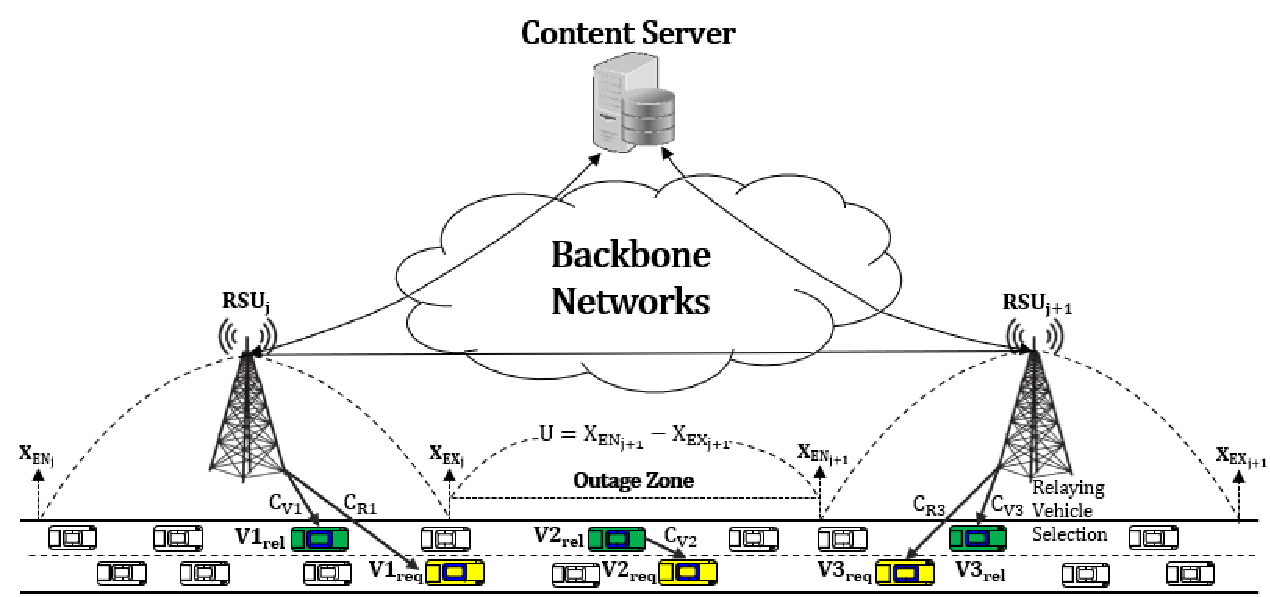
\includegraphics[width=14 cm]{figure/Fig1.pdf}}
\caption{The network model and the overview of the proposed scheme.}
\label{fig1}
\end{figure}
\newpage
If a vehicle requires to download the intended content while moving in the communication coverage of the RSU where the vehicle is located, the vehicle sends an interest packet to the RSU to request the intended content. In this paper, we named a vehicle that sends an interest packet to an RSU to download the intended content as a requester vehicle. Upon receiving the packet showing interest, the RSU requests and receives the intended content to and from the corresponding content server. After receiving the intended content, the RSU determines whether it can download the entire intended content to the requester vehicle. For this purpose, the proposed scheme calculates the downloadable amount of content for a requester vehicle in the communication coverage of the RSU where the requester vehicle is located. Then, the downloadable amount of content is calculated using the mobility information of the requester vehicle and the V2I transmission rate of the RSU. If the RSU can download the entire content to the requester vehicle, it sends the content to the requester vehicle. However, if the RSU cannot download the entire content to the requester vehicle, it selects the optimal relaying vehicle among vehicles except the requester vehicle in its communication coverage to precache the intended content for the requester vehicle. In the proposed scheme, the optimal relaying vehicle is determined by calculating both the downloadable time and amount from the RSU, and the relaying time and amount between the requester vehicle and each relaying vehicle. The RSU then precaches the optimal relaying amount of the intended content to the optimal relaying vehicle. Thus, the requester vehicle downloads the intended content from the RSU up to the amount that the RSU is enabled for sending. After exiting the communication coverage of the RSU, the requester vehicle receives the optimal relaying amount of intended content from the optimal relaying vehicle in the outage zone. Although the requester vehicle cannot fully download the entire size of the intended content from both the RSU and the optimal relaying vehicle, the RSU precaches the remaining amount of the intended content to the next RSU on the predicted trajectory of the requester vehicle through backhaul links. Thus, when the requester vehicle enters the next RSU, it can immediately download the remaining amount of intended content from the next RSU. If the next RSU cannot download the remaining amount of the intended content to the requester vehicle in its communication coverage, the aforementioned process continues until the downloading of the intended content is completed. Figure~\ref{fig1} shows an overview of the proposed scheme to describe the cooperative content precaching process based on both the optimal relaying vehicle and the next downloading RSU. The proposed scheme is described in detail in Section \ref{sec3}.


\section{The Selection of the Optimal Relaying Vehicle} \label{sec3}
In this section, we describe the precaching scheme by selecting the optimal relaying vehicle and next RSU to provide as much content as possible to the requester vehicle. We first explain the decision to use precaching based on the downloadable amount of content in Section \ref{sec3.1}. Then, we select the optimal relaying vehicle based on the connectivity prediction in Section \ref{sec3.2}. Finally, in Section \ref{sec3.3}, we explain how the next RSU precaches the content to provide it to the requester vehicle.
Table \ref{tab.1}~shows notations for selecting the optimal relaying vehicle.


\begin{table}[H] % table1
\tablesize{\footnotesize}

  \caption{Notations for selecting the optimal relaying vehicle.}

\setlength{\cellWidtha}{\textwidth/2-2\tabcolsep-2.2in}
\setlength{\cellWidthb}{\textwidth/2-2\tabcolsep+2.2in}
\scalebox{1}[1]{\begin{tabularx}{\textwidth}{>{\centering\arraybackslash}m{\cellWidtha}>{\raggedright
\arraybackslash}m{\cellWidthb}}
\toprule

           \textbf{Notation} & \textbf{Description}\\
\midrule
        $RSU_{j}$ & $j$-th roadside unit (RSU), where $j\in \{1, \cdots, J\}$\\
        $V_{i}$ & $i$-th vehicle, where $i \in \{1, \cdots, I\}$ \\
        $V_{req}$ & The requester vehicle\\
        $V_{rel}$ & The selected optimal relaying vehicle\\
        $t_{max\_i}$ & The maximum time that $V_{i}$ can relay the content to $V_{req}$ within the outage zone \\
        $t_{D_{req}}$ & The downloadable time for providing the requested content to $V_{req}$ within the coverage of $RSU_{j}$ \\
        $T_{D_{i}}$ & The downloadable time for precaching the requested content to $V_{i}$ within the coverage of $RSU_{j}$ \\
        $T_{R_{i}}$ & The relaying time of $V_{i}$ for providing the precached content to $V_{req}$ within the outage zone \\
        $x_{EX_{j}}$ & The coverage diameter of $RSU_{j}$ \\
        $x_{req}$ & The current location of $V_{req}$ \\


   \bottomrule
    \end{tabularx}}
%\end{adjustwidth}
    \label{tab.1}
\end{table}



\begin{table}[H] \ContinuedFloat % table1
\tablesize{\footnotesize}

  \caption{{\em Cont.}}

\setlength{\cellWidtha}{\textwidth/2-2\tabcolsep-2.2in}
\setlength{\cellWidthb}{\textwidth/2-2\tabcolsep+2.2in}
\scalebox{1}[1]{\begin{tabularx}{\textwidth}{>{\centering\arraybackslash}m{\cellWidtha}>{\raggedright
\arraybackslash}m{\cellWidthb}}
\toprule

           \textbf{Notation} & \textbf{Description}\\
\midrule
        $x_{i}$ & The current location of $V_{i}$ \\
        $v_{req}$ & The current speed of $V_{req}$ \\
        $v_{i}$ & The current speed of $V_{i}$ \\

        $R_{I2V}$ & The transmission rate of the I2V \\
        $R_{V2V}$ & The transmission rate of the V2V \\
        $C_{T}$ & The total size of the requested content\\
        $C_{R}$ & The downloadable amount of the requested content for providing the requested content to $V_{req}$ within the coverage of $RSU_{j}$ \\
        $C_{DV_{i}}$ & The downloadable amount of the requested content for precaching it to $V_{i}$ within the coverage of $RSU_{j}$ \\
        $C_{RV_{i}}$ & The relaying amount of the content for providing it to $V_{req}$ within the outage zone \\
        $C_{PDV_{i}}$ & The maximum amount of the requested content for providing it from $V_{i}$ to $V_{req}$ within the outage zone by precaching it to from $RSU_{j}$ to $V_{i}$ within the coverage of $RSU_{j}$ \\
        $C_{V}$ & The relaying amount of the precached content for providing it to $V_{req}$ within the outage zone \\
        $r_{c}$ & The coverage radius of the vehicles\\
        $U$ & The distance of the outage zone between $RSU_{j}$ and $RSU_{j+1}$\\

   \bottomrule
    \end{tabularx}}
%\end{adjustwidth}
    \label{tab.1}
\end{table}



\subsection{Checking the Necessity for Precaching} \label{sec3.1}
If a vehicle traveling on the road within the coverage area of $RSU_{j}$ wants to download the content, it sends a request message to $RSU_{j}$, where $j=\{1, \cdots, J\}$.
When $RSU_{j}$ receives the request message from the requester vehicle $V_{req}$, it calculates the downloadable time ${t}_{{D}_{req}}$ that $V_{req}$ can download the content from the $RSU_{j}$ within its coverage.
${t}_{{D}_{req}}$ can be denoted as the time at which $V_{req}$ is expected to leave $RSU_{j}$'s coverage, and it can be calculated based on the velocity and the location of $V_{req}$ as follows:
\begin{equation}
     {t}_{{D}_{req}}=\cfrac{{x}_{{EX}_{j}}-{x}_{req}}{{v}_{req}}, % eq 1
\end{equation}
where ${x}_{{EX}_{j}}$ is the communication coverage of the $RSU_{j}$, $x_{req}$ is the location of $V_{req}$, and $v_{req}$ is the velocity of $V_{req}$, respectively.
Based on $t_{D_{req}}$, $RSU_{j}$ calculates the downloadable amount ${C}_{R}$ of the requested content that can be provided to the $V_{req}$ within $RSU_{j}$'s coverage by using the transmission rate of the I2V communication, as follows:
\begin{equation}
     {C}_{R}={t}_{{D}_{req}} \times {R}_{I2V}, % eq 2 
\end{equation}
where $R_{I2V}$ is the transmission rate of the I2V based on IEEE 802.11p WAVE~\cite{wave2016}.

$RSU_{j}$ then decides whether the requested content has to be precached by comparing $C_{R}$ with $C_{T}$.
If ${C}_{T}\leq{C}_{R}$, it denotes that $RSU_{j}$ can provide all of the requested content to $V_{req}$ before $V_{req}$ leaves the communication coverage of $RSU_{j}$, where $C_{T}$ is the size of the requested content by $V_{req}$.
In this case, $RSU_{j}$ immediately provides the requested content to $V_{req}$.
Otherwise, it denotes that $RSU_{j}$ does not have sufficient time to provide all of the requested content to $V_{req}$ at time $t_{D_{req}}$.
Thus, $RSU_{j}$ should select a relaying vehicle among the vehicles within its coverage to provide the requested content to $V_{req}$ after $V_{req}$ leaves the coverage of $RSU_{j}$.
The relaying vehicle, $V_{rel}$, provides the remaining amount of content to $V_{req}$ outside the communication coverage of $RSU_{j}$.
% We describe the selection of the optimal relaying vehicle in Section \ref{sec3.2}.
% It is possible that $RSU_{j}$ and $V_{rel}$ can not provide all the requested content to $V_{req}$ due to the huge size of the content or the short connectivity.
% In that case, the requested content has to be precached at the next RSU based on the trajectory of $V_{req}$.
% Therefore, we present how to precache the content to the next RSU in Section \ref{sec3.3}.


\subsection{Selection of the Optimal Relaying Vehicle} \label{sec3.2}
In this section, we describe the selection of the optimal relaying vehicle to provide the remaining requested content to $V_{req}$.
It is possible that $RSU_{j}$ and $V_{rel}$ cannot provide all the requested content to $V_{req}$ owing to the large size of the content or the short connectivity.
In this case, to provide the remaining amount of content to $V_{req}$ outside the coverage, $RSU_{j}$ should select the relaying vehicle while providing as much requested content as possible to $V_{req}$ within its coverage.
To determine the optimal relaying vehicle $V_{rel}$, $RSU_{j}$ calculates the amount of the content that can be relayed by each candidate vehicle that is managed by the table of $RSU_{j}$ within its coverage.
Then, $RSU_{j}$ selects the optimal relaying vehicle among the candidate vehicles and the amount $C_{V}$ of the requested content that can be relayed by~it.

% In many cases, it might be ${C}_{V}\leq({C}_{T} - {C}_{R})$.
% For example, as shown Fig. 1, ${RSU}_{j}$ delivers ${C}_{R1}$ to ${V1}_{req}$, selects ${V1}_{rel}$ with ${C}_{V1}$ as its relaying vehicle, and sends ${C}_{V1}$ to ${V1}_{rel}$. In the outage zone between ${RSU}_{j}$ and ${RSU}_{j+1}$, ${V1}_{rel}$ relays ${C}_{V1}$ to ${V1}_{req}$.

For this selection through the table, $RSU_{j}$ uses the beacon messages that include the mobility information of vehicles that remain in the coverage of $RSU_{j}$.
Based on the location and velocity of each candidate vehicle, $RSU_{j}$ calculates each candidate vehicle's downloadable time and the downloadable amount of the content from $RSU_{j}$, as shown in Section \ref{sec3.2.1}.
It also calculates the relaying time and the relaying amount of the content, which can be relayed to $V_{req}$ from each candidate vehicle, as detailed in Section \ref{sec3.2.2}.
In Section \ref{sec3.2.3}, using these values, $RSU_{j}$ selects the optimal relaying vehicle as $V_{rel}$ and its relaying amount as $C_{V}$.
Therefore, $RSU_{j}$ provides the $C_{V}$ of the content to $V_{rel}$ within its coverage and $V_{rel}$ relays it to $V_{req}$ when $V_{req}$ leaves $RSU_{j}$'s coverage.


\subsubsection{The Downloadable Time and Amount} \label{sec3.2.1}
To determine the optimal relaying vehicle $V_{rel}$, $RSU_{j}$ first has to know the downloadable time and amount of the content of each candidate vehicle $V_{i}$ within $RSU_{j}$'s coverage.
Similarly, to obtain ${T}_{{D}_{req}}$, the downloadable time of each candidate vehicle can be calculated based on $x_{EX_{j}}$.
However, when $V_{req}$ leaves the coverage of $RSU_{j}$, the content must be relayed to $V_{req}$ from the relaying vehicle.
Therefore, $RSU_{j}$ can obtain the downloadable time of each candidate vehicle from $RSU_{j}$ in order to provide it to $V_{req}$, as follows:
\begin{equation}
     {T}_{{D}_{i}}=min \left( \cfrac{{x}_{{EX}_{j}}-{x}_{i}}{{v}_{i}}, t_{D_{req}} \right), % eq 4
\end{equation}
where ${x}_{i}$ and ${v}_{i}$ are the position and speed of ${V}_{i}$, respectively.
Then, $RSU_{j}$ calculates the downloadable amount $C_{DV_{i}}$ of the content that the $V_{i}$ can precache from $RSU_{j}$ during the time ${T}_{{D}_{i}}$ based on the transmission rate of I2V as follows:
\begin{equation}
     {C}_{{DV}_{i}}={T}_{{D}_{i}}\times{R}_{I2V}, % eq 5
\end{equation}
where ${R}_{I2V}$ is the V2I transmission rate that is based on IEEE 802.11p WAVE~\cite{wave2016}.
Even if $V_{i}$ can precache the $C_{DV_{i}}$ of the content, it may not relay it to $V_{req}$ because of the short connectivity between $V_{req}$ and $V_{rel}$.
Hence, the relaying time and amount of content must be calculated.

\subsubsection{The Relaying Time and Amount} \label{sec3.2.2}
It is also necessary to calculate the relaying time and relaying amount of the requested content of the candidate vehicles in the outage zone to select the optimal relaying vehicle. To determine the relaying time, $RSU_{j}$ must first calculate the connection time between $V_{req}$ and each $V_{i}$.
However, when $V_{req}$ enters the next RSU, that is, $RSU_{j+1}$'s coverage, the download from the $RSU_{j+1}$ is better than that from $V_{i}$, owing to the difference in the power and the transmission performances.
Therefore, the relaying should be conducted within the outage zone, which is the area between the coverages of $RSU_{j}$ and $RSU_{j+1}$. Then, the relaying time ${T}_{{R}_{i}}$ of $V_{i}$ can be denoted based on the location and the velocity of both $V_{req}$ and $V_{i}$, as follows:
\begin{equation}
{T}_{{R}_{i}}=
    \begin{cases} % eq 6
        \cfrac{{r}_{c}+{x}_{i}-{x}_{req}}{{v}_{req}-{v}_{i}} - {T}_{{D}_{i}}, & if {v}_{req} > {v}_{i}\\
        \cfrac{{r}_{c}-{x}_{i}-{x}_{req}}{{v}_{req}-{v}_{i}} - {T}_{{D}_{i}}, & if {v}_{req} < {v}_{i}\\ 
        {t}_{max\_i}, & if {v}_{req} = {v}_{i}
    \end{cases},
\end{equation}
where ${r}_{c}$ is the communication range of the vehicles, ${x}_{i}$ is the location of $V_{i}$, and $v_{i}$ is the velocity of $V_{i}$. ${T}_{{D}_{i}}$ is the downloadable time of ${V}_{i}$.
${t}_{max\_i}$ is the maximum time that $V_{i}$ can relay the content to $V_{req}$ within the outage zone.
However, if the relaying time $T_{R_{i}}$ of $V_{i}$ is larger than ${t}_{max\_i}$, then $T_{R_{i}}$ is limited to ${t}_{max\_i}$.
${t}_{max\_i}$ is denoted as follows:
\begin{equation}
     {t}_{max\_i}=\cfrac{U}{{v}_{req}} - {T}_{{D}_{i}}, % eq 7
\end{equation}
where $U$ is the distance of the outage zone between the ${RSU}_{j}$ and ${RSU}_{(j+1)}$.
This indicates that $V_{req}$ can receive the content from the selected $V_{i}$ within the outage zone and from  $RSU_{j+1}$ after passing through the outage zone.
Using $T_{R_{i}}$, $RSU_{j}$ can calculate the relaying amount ${C}_{{RV}_{i}}$ of the  content  that can be provided to $V_{req}$ from $V_{i}$ within the outage zone, as~follows:
% However, in the ${RSU}_{(j+1)}$ coverage, ${V}_{req}$ is better to receive the remaining amount of the corresponding content from ${RSU}_{(j+1)}$ than ${V}_{i}$, because ${RSU}_{(j+1)}$ can send the content with a high transmission rate to ${V}_{req}$ in the ${RSU}_{(j+1)}$ coverage. 
%Thus, if ${T}_{{R}_{i}}$ is higher than ${t}_{max\_i}$, ${RSU}_{j}$ replaces ${T}_{{R}_{i}}$ with ${t}_{max\_i}$. In other word, if ${T}_{{R}_{i}} > {t}_{max\_i}$, ${T}_{{R}_{i}} = {t}_{max\_i}$.
\begin{equation}
     {C}_{{RV}_{i}}={T}_{{R}_{i}}\times{R}_{V2V}, % eq 8
\end{equation}
where ${R}_{V2V}$ is the transmission rate of the V2V communications that is based on IEEE 802.11p WAVE~\cite{wave2016}.
$RSU_{j}$ can select the optimal relaying vehicle $V_{rel}$ because it now knows the amount of the content that can be downloaded to $V_{i}$ from $RSU_{j}$ and can be relayed to $V_{req}$ from $V_{i}$.


\subsubsection{Selection of the Optimal Relaying Vehicle} \label{sec3.2.3}
To select the optimal relaying vehicle, $RSU_{j}$ creates each set of $V_{i}$ using the downloadable amount ${C}_{{DV}_{i}}$ and the relaying amount ${C}_{{RV}_{i}}$ of the content as follows:
\begin{equation}
    Set({V}_{i})=\{{C}_{{DV}_{i}},{C}_{{RV}_{i}}\}.% eq 9
\end{equation}

The set $Set(V_{i})$ is saved in the $RSU_{j}$'s table with the mobility information of $V_{i}$.
Based on $Set(V_{i})$, $RSU_{j}$ compares the ${C}_{{DV}_{i}}$ and ${C}_{{RV}_{i}}$ of each $V_{i}$ and selects a smaller value.
In the case of ${C}_{{DV}_{i}} > {C}_{{RV}_{i}}$, it denotes that the connection time between $V_{req}$ and $V_{i}$ is insufficient to relay all the precached content that $V_{i}$ downloads from $RSU_{j}$.
Otherwise, in the case of ${C}_{{DV}_{i}} < {C}_{{RV}_{i}}$, it denotes that the downloadable time of $V_{i}$ is not sufficient to compare the connection time that $V_{i}$ can provide the content to $V_{req}$.
Therefore, $RSU_{j}$ selects the minimum value between the two values as the practical delivery amount ${C}_{{PDV}_{i}}$ of the content, as follows:
\begin{equation}
    {C}_{{PDV}_{i}}=min\{{C}_{{DV}_{i}},{C}_{{RV}_{i}}\}. % eq 10
\end{equation}

Thus, $C_{PDV_{i}}$ denotes that the maximum amount of the content that $V_{i}$ can practically provide to $V_{req}$ before $V_{req}$ reaches the coverage of $RSU_{j+1}$.
Then, $RSU_{j}$ can determine the optimal relaying amount ${C}_{V}$ by selecting the optimal relaying vehicle that has the largest $C_{PDV_{i}}$, as follows:
\begin{equation}
    {C}_{V}={C}_{{PDV}_{rel}}=max\{{C}_{{PDV}_{1}}, \cdots,{C}_{{PDV}_{n}}\}. % eq 11
\end{equation}

The ${C}_{{PDV}_{rel}}$ of ${V}_{rel}$ denotes the maximum amount of the content that $V_{req}$ can receive from $V_{rel}$ within the outage zone.

When $V_{req}$ leaves the coverage of $RSU_{j}$ and enters the outage zone, $V_{rel}$ immediately provides the $C_{V}$ of downloaded content to $V_{req}$.
For example, as shown in Figure \ref{fig1}, if $V1_{rel}$ is selected as the optimal relaying vehicle for $V1_{req}$, because $V1_{req}$ wants to download the content, $RSU_{j}$ provides the $C_{R}$ of the requested content to $V1_{req}$ and the $C_{V}$ of the requested content to $V_{rel}$.
Then, in the case of $V2_{rel}$, which is selected as the optimal relaying vehicle for $V2_{req}$ and downloaded $C_{V}$ of the content, it provides the content to $V2_{req}$ during the outage zone.


\subsection{Optimal Content Precaching to Next RSU} \label{sec3.3}
If the $C_{R}+C_{V}$ is smaller than $C_{T}$, which is the total size of the requested content, $RSU_{j}$ judges that it is not sufficient for the content that can be provided before $V_{req}$ reaches $RSU_{j+1}$.
In this case, $RSU_{j}$ sends a message to make the next RSU, that is, $RSU_{j+1}$ precaches the remaining amount of the requested content.
The amount $C_{P}$ of the content that must be precached at $RSU_{j+1}$ can be easily determined based on $C_{T}$, $C_{R}$, and $C_{V}$ as follows:
\begin{equation}
     {C}_{P}={C}_{T} - {C}_{R} - {C}_{V}.  % eq 12
\end{equation}

Therefore, the message that $RSU_{j}$ sends to $RSU_{j+1}$ via the backhaul network includes the name and the amount $C_{P}$ of the requested content and the information about $V_{req}$.
If there are no candidate vehicles that can relay the content to $V_{req}$, the amount $C_{P}$ becomes ${C}_{T} - {C}_{R}$.
When the $V_{req}$ enters into $RSU_{j+1}$'s coverage, ${RSU}_{j+1}$ immediately provides the $C_{P}$ of the requested content that has already been precached.
Then, $V_{req}$ receives all the requested content through all RSUs, including $RSU_{j+1}$.
For example, as shown in Figure \ref{fig1}, if $V3_{rel}$ is selected as the optimal relaying vehicle for $V3_{req}$ because $V3_{req}$ has to receive a greater amount of the requested content, $RSU_{j}$ provides the $C_{R}$ of the requested content to $V3_{req}$ and the $C_{V}$ of the requested content to $V_{rel}$.

In a summary, Algorithm \ref{table1} briefly describes the cooperative content precaching of the proposed scheme.
Line 1 defines $C_{T}$ using the information about the content $c$.
Lines 2--5 compare $C_{T}$ and the downloadable size $C_{R}$ within the RSU $j$'s coverage to decide the usage of precaching, as shown in Section \ref{sec3.1}.
Lines 6--15 select the optimal relay vehicle $V_{rel}$ to precache $c$ to provide it to $V_{req}$ as described in Section \ref{sec3.2}.
Lines 16--17 explain the optimal precaching to the next RSU as discussed in Section \ref{sec3.3}.

\begin{algorithm}[H]

    \caption{Cooperative Content Precaching} \label{table1}
    \textbf{Input: } the content $c$, the RSU $j$'s coverage $x_{EX_{j}}$, the requester vehicle $V_{req}$'s the location $x_{req}$ and the velocity $v_{req}$\\
    \textbf{Output: } Action of the RSU $j$
    \begin{algorithmic}[1]
        \State $C_{T} \leftarrow ($the size of $c)$
        \State $C_{R} \leftarrow C_{R}(x_{EX_{j}}, x_{req}, v_{req})$
        \If {$C_{T} \leq C_{R}$}
            \State [Providing $C_{T}$-sized $c$ to $V_{req}$]
        \Else
            \State $max = maxID = 0$
            \For {$i \in {1, \cdots, n}$}
                \State $C_{PDV, i} = min\{C_{DV_{i}}, C_{RV_{i}}\}$
                \If {$C_{PDV_{i}} > max$}
                    \State $max$ = $C{PDV_{i}}$
                    \State $maxID$ = $i$
                \EndIf
                \State $V_{rel} \leftarrow maxID$
                \State $C_{V}$ = $max$
                \State [Providing $C_{R}$-sized $c$ to $V_{req}$]
                \State [Precaching $C_{V}$-sized $c$ to $V_{rel}$]
                \If {$C_{T}>C_{R}+C_{V}$}
                    \State [Sending ($V_{req}$, $C_{R}+C_{V}$, $c$) information to the RSU $j+1$]
                \EndIf
            \EndFor
        \EndIf
    \end{algorithmic}
\end{algorithm}



\section{Guardband for Handling the Mobility Prediction Errors} \label{sec4}
To select the optimal relaying vehicle, the proposed scheme must calculate the downloadable time of a requester vehicle ${V}_{req}$ in an RSU and the relaying time between ${V}_{req}$ and the relaying vehicle ${V}_{rel}$ in the outage zone. The downloadable time is based on the dwell time of ${V}_{req}$ in the RSU and the relaying time is based on the contact time between ${V}_{req}$ and ${V}_{rel}$.
However, accurately predicting both dwell and contact times is very difficult because vehicles change their speed irregularly. In this section, we describe a guardband to compensate for the mobility prediction error caused by the fact that accurately predicting dwell and contact times is not feasible. An error exists in predicting the connection time (the contact time between vehicles in an outage zone and the dwell time of a requester vehicle ${V}_{req}$ in an RSU) based on their speed.
Two mobility-prediction errors arise when the connection time is inaccurate. First, due to the shorter-than-expected download time in an RSU, $V_{req}$ does not obtain the expected amount of precached content. Because the portion of the content that is not received is not precached in the next RSU, the next RSU must obtain it from the content server or the previous RSU and send it to $V_{req}$.
Obtaining content from the content server causes an additional delay. Second, the relay time between $V_{req}$ and $V_{rel}$ in the outage zone may deviate from the predicted value. If it is shorter than expected, the network performance will decrease for the same reason stated earlier. If the relaying time is longer than expected, $V_{rel}$ cannot provide extra content because it has only a precached portion of the content. In this instance, the delay increases owing to the increased time, which is required to provide the requested content. Therefore, a guardband against prediction errors of the contact time between vehicles can mitigate the corresponding problem.
Table \ref{tab.2} shows notations for the calculation of the guardband.

In this study, there are two situations that predict the connection time: (1) in Section~\ref{sec4.1}, the dwell time of ${V}_{req}$ within the RSU communication range is calculated; (2) in Section~\ref{sec4.2}, the contact time between ${V}_{req}$ and ${V}_{rel}$ outside the RSU range is determined. These two estimated connection times can be used to formulate the number of guardbands required, as shown in Section~\ref{sec4.3}.


\begin{table}[H] % table1
\tablesize{\footnotesize}

    \caption{Notations for the calculation of the guardband.}
 \setlength{\cellWidtha}{\textwidth/2-2\tabcolsep-1.6in}
\setlength{\cellWidthb}{\textwidth/2-2\tabcolsep+1.6in}
\scalebox{1}[1]{\begin{tabularx}{\textwidth}{>{\centering\arraybackslash}m{\cellWidtha}>{\raggedright
\arraybackslash}m{\cellWidthb}}
\toprule

        \textbf{Notation} & \textbf{Description} \\
       \midrule

        $delay_{E\_re}(G, \varepsilon_{mob})$ & The expected reduced delay value by $G$ of guardband and $\varepsilon_{mob}$ of mobility error~ratio \\
        $t_{theo}$ & The theoretical delay value in an ideal situation \\
        $t_{est}$ & The actual estimated delay value that is obtained by the predicted situation \\
        $m_{theo}$ & The theoretical distance value in an ideal situation \\
        $m_{est}$ & The actual estimated distance value that is obtained by the predicted situation \\
        $l$ & The transmission rate of backhaul links \\
        $\xi_{req, j}(m)$ & One or zero value whether $RSU_{j}$ provides the requested content to $V_{req}$ after $V_{req}$ moves a distance of $m$ meters\\
        %MDPI: Please confirm if the highlighted parts in this Table is necessary. iF not, please remove them.
        $\delta_{req, k}(m)$ & One or zero value whether $V_{k}$ provides the precached content to $V_{req}$ after $V_{req}$ moves a distance of $m$ meters \\
        $\varepsilon_{mob}$ & The mobility error ratio of the vehicles \\
        $v_{req}(j)$ & The expected speed based on $v_{req}$ at the coverage of $RSU_{j}$ \\
        $v_{req, av}(j)$ & The average expected speed based on $v_{req}$ and $\varepsilon_{mob}$ at the coverage of $RSU_{j}$ \\
        $v^{out}_{req, av}(j)$ & The average expected speed based on $v_{req}$ and $\varepsilon_{mob}$ at the outage zone between $RSU_{j}$ and $RSU_{j+1}$ \\
  $v^{out}_{i, av}(j)$ & The average expected speed based on $v_{i}$ and $\varepsilon_{mob}$ at the outage zone between $RSU_{j}$ and $RSU_{j+1}$ \\
        $R_{req, j}(m)$ & One or zero value whether $RSU_{j}$ relays the requested content to $V_{req}$ after $V_{req}$ moves a distance of $m$ meters \\
        $P_{req, k}(m)$ & One or zero value whether $V_{k}$ provides the precached content to $V_{req}$ after $V_{req}$ moves a distance of $m$ meters \\
        $conn_{req, j}(m)$ & One or zero value whether $V_{req}$ and $RSU_{j}$ are connected after $V_{req}$ moves a distance of $m$ meters \\
        $out_{req, j}(m)$ & One or zero value whether $V_{req}$ stays within the outage zone between $RSU_{j}$ and $RSU_{j+1}$ after $V_{req}$ moves a distance of $m$ meters \\
        $traffic_{E\_re}(G, \varepsilon_{mob})$ & The expected reduced traffic by $G$ of guardband and $\varepsilon_{mob}$ of mobility error ratio \\
        $traffic_{theo}$ & The theoretical traffic value in ideal situation \\
        $traffic_{est}$ & The actual estimated traffic value that is obtained by the predicted situation \\

     \bottomrule
\end{tabularx}}

    \label{tab.2}
\end{table}

\subsection{Dwell Time in an RSU} \label{sec4.1}
When ${V}_{req}$ enters the coverage area of an RSU, its dwell time can be calculated using its position, velocity, and trajectory information. The proposed scheme then determines the amount of content ${V}_{req}$ can download from the current RSU throughout its dwell time. Therefore, the proposed scheme allows the current RSU to precache the remaining portion of the requested content to the next RSU for ${V}_{req}$. The remaining content is the total amount of content minus the amount of content downloaded during dwell time. However, if ${V}_{req}$ increases its speed and, as a result, its dwell time decreases, the practical amount that can be downloaded is also reduced. Hence, when ${V}_{req}$ connects to the next RSU, it should retrieve from the content server and transmit to ${V}_{req}$ the portions of the content that were not received by ${V}_{req}$ in the previous RSU. Because the data rate at which the content is brought from the content server and delivered to ${V}_{req}$ is slower than the data rate at which the precached content is delivered directly to ${V}_{req}$, this situation causes an additional delay for the content download. Thus, the next RSU can prevent this additional delay by preparing a guardband by considering the amount of content that cannot be received by ${V}_{req}$ in the previous RSU.

On the contrary, if the dwell time of ${V}_{req}$ is increased because of its increased speed, it can download a higher amount of content from the current RSU than expected. In this situation, ${V}_{req}$ can download a portion of the precached content that was already sent to the next RSU from the current RSU during the dwell time. Then, when ${V}_{req}$ connects to the next RSU, it does not need to download a portion of the content from the next RSU. Thus, ${V}_{req}$ can obtain the time required to download an additional amount of content from the next RSU. In particular, because the amount of precached content to the next RSU was already determined by the previous RSU, the additional amount that can be downloaded should be taken from the content server to the next RSU and delivered from the next RSU to ${V}_{req}$. This process is very inefficient in terms of the data rate and results in many delays. Therefore, preparing a guardband at the next RSU to download the additional amount can reduce delays.


\subsection{Contact Time with the Relaying Vehicle} \label{sec4.2}
The dwell time between ${V}_{req}$ and an RSU within the RSU coverage was calculated using the mobility prediction of ${V}_{req}$. The contact time between the vehicles within the outage zone was calculated using the mobility predictions of both ${V}_{req}$ and the candidate vehicle. Therefore, the contact time has more prediction errors, as it is more difficult to predict. Two scenarios can occur in terms of mobility prediction error. First, if the speed of ${V}_{req}$ decreases, the contact time between ${V}_{req}$ and ${V}_{rel}$ increases and the arrival time to the next RSU increases. However, ${V}_{rel}$ cannot send an additional amount of content to ${V}_{req}$ during the increased contact time because it has received only the precached amount of content. Hence, it results in a delay wherein ${V}_{req}$ does not receive the additional amount of the content after it finishes receiving the precached amount of the content from ${V}_{rel}$. Thus, preparing the guardband in advance for the potentially increased contact time can reduce the overall delay because the additional content in the guardband can be provided to ${V}_{req}$ when the contact time increases. Subsequently, if ${V}_{req}$ has a higher speed than the expected speed and does not receive certain portions of the content to download from the current RSU, ${V}_{rel}$ is not able to send the portion to ${V}_{req}$ because ${V}_{rel}$ has only the precached amount of the content. Therefore, the next RSU should provide a portion of the content to ${V}_{req}$ preferentially before it provides its own precached amount of content. This causes an additional delay because the next RSU must take a portion of the content from the previous RSU or the content server. Therefore, if ${V}_{rel}$ has a portion of the content as a guardband, it reduces the burden on the next RSU and additional delay.

Consequently, if both ${V}_{rel}$ and the next RSU prepare a guardband for the content to be precached, the overall burden of the RSU is reduced because it can immediately send the guardband to ${V}_{req}$ without using the content server or the previous RSU. In addition, the guardband can increase the hit ratio to download the content when an error occurs. Furthermore, the guardband is very efficient in reducing the time delay involved in downloading the entire content by ${V}_{req}$.

\subsection{Calculation of the Guardband} \label{sec4.3}
To use the guardband of precached content, we need to determine how much it needs to be prepared. We can minimize the delay that the requester vehicle may experience when the next RSU allocates the remaining portion of the requested content as a guardband. However, this causes a significant consumption of traffic. The unused guardband is discarded as wasted traffic. Consequently, there should be a proper trade-off between traffic and delay, according to the guardband.

The delay must be calculated first because the amount of traffic consumed is calculated by the delay. In this study, the delay was calculated using the mobility information of the requester vehicle, the size of the precached content, and the size of the guardband. The expected reduced delay value $delay_{E\_re}(G, \varepsilon_{mob})$ according to the guardband can be obtained by the difference between the theoretical delay value ${t}_{theo}$ and the actual estimated delay value, ${t}_{est}$. Thus, we need to calculate both ${t}_{theo}$ and ${t}_{est}$.

First, the theoretical delay value ${t}_{theo}$ consumed for content download is predicted by using the current speed of the requester vehicle.
To derive $t_{theo}$ based on the total size of the requested content and the transmission rate of the RSUs, the speed of $V_{req}$ and the distance that $V_{req}$ moves are used rather than the connection time. From this point of view, because the time that $V_{req}$ traveled 1 m at the speed of $v_{req}$ is $v_{req}^{-1}$, the size at which $V_{req}$ receives the requested content from an RSU is $R_{V2I} \times v_{req}^{-1}$.
The first RSU, $RSU_{1}$, should receive the requested content from the content server via backhaul links before providing it to $V_{req}$.
In this case, the size at which $V_{req}$ can receive content from $RSU_{1}$ is $(R_{V2I}^{-1} + l^{-1})^{-1} \times v_{req}^{-1}$, where $l$ is the transmission rate of the backhaul link.
However, because $t_{theo}$ is a time value, the theoretical distance value $m_{theo}$ consumed for content download should be defined first.
Here, $t_{theo}$ is $m_{theo} / v_{req}$, where $v_{req}$ is the speed of $V_{req}$.
Therefore, the relationship between the $C_{T}$ and $m_{theo}$ is defined as follows:
\begin{equation}
    \begin{split}
        C_{T}&=\sum_{m=0}^{m_{1}}\left( (R_{V2I}^{-1} + l^{-1})^{-1} \cdot\cfrac{\xi_{req, 1}(m)}{v_{req}}\right) \\
        &+\sum_{j=2}^{J}\sum_{m=m_{1}}^{m_{theo}}\left(R_{V2V}\cdot\cfrac{\sum_{k=1}^{K_{req,j-1}}\delta_{req, k}(m)}{v_{req}}+R_{V2I}\cdot\cfrac{\xi_{req, j}(m)}{v_{req}} \right) ,
    \end{split}
\end{equation}
where ${\xi}_{req, j}(m)$ denotes whether $RSU_{j}$ provides the requested content to $V_{req}$ after $V_{req}$ moves a distance of $m$ m. If $RSU_{j}$ provides the requested content to $V_{req}$ after $V_{req}$ moves $m$ m, ${\xi}_{req, j}(m)$ is one. Otherwise, ${\xi}_{req, j}(t)$ is zero. ${R}_{V2I}$ is the transmission rate between an RSU and a vehicle. $l$ is the transmission rate of backhaul links. ${\delta}_{req, k}(m)$ indicates whether ${V}_{rel}$ communicates with ${V}_{req}$ after $V_{req}$ moves $m$ m. ${\xi}_{req, j}(m)$ and ${\delta}_{req, k}(m)$ can be either zero or one.
$m_{1}$ is the distance at which $V_{req}$ reaches the end of the $RSU_{1}$'s coverage.
To calculate ${t}_{theo}$, ${\xi}_{req, j}(m)$ and ${\delta}_{req, k}(m)$ can be known in advance because the mobility information of the vehicles is provided to the RSUs by accessing the server that manages the mobility information.
The first sum represents the size of the content that $RSU_{1}$ receives from the content server over the backhaul link and provides to $V_{req}$.
The second sum represents the sizes of the content that $V_{k}$ and $RSU_{j}$ provide $V_{req}$.
In addition, because each node does not have an overlapped connection (in other words, a node cannot connect with another vehicle during connecting one vehicle), $\sum_{j=1}^{J}\sum_{k=1}^{K_{req,j-1}}(\delta_{req, k}(m)+\xi_{req, j}(m))\leq 1, \forall{m}$. $K_{req,j-1}$ is the number of candidate vehicles that can become relaying vehicles within the coverage of $RSU_{j-1}$.
In addition, because all values in sigma except ${\xi}_{req, j}(m)$ are fixed, $C_{T}$ is derived through the sum of values that are defined by ${\xi}_{req, j}(m)$, which can be zero or one. In addition, if the requester vehicle remains within $RSU_{j}$’s communication coverage at each m, ${\xi}_{req, j}(m)$ must be 1.
The relaying vehicle selection is conducted only outside the coverage of RSUs, where only vehicles that can provide the requested content to $V_{req}$ at each $m$ are considered candidate vehicles for the relaying vehicle.
At each $m$, because only one vehicle is selected among the candidate relaying vehicles, $\sum_{k=1}^{K_{req,j-1}} \delta_{req, k}(m)$ cannot be greater than one.
Moreover, when there are no candidate vehicles that can provide the requested content to the requester vehicle, $\sum_{k=1}^{K_{req,j-1}} \delta_{req, k}(m)$ becomes 0
Based on these constraints, the optimal ${\xi}_{req, j}(m)$ can be calculated.
The difference between ${t}_{theo}$ and the actual estimated content download delay ${t}_{est}$ depends on the magnitude of the mobility prediction error with respect to speed. The mobility prediction error for speed $v_{req}$ of the requester vehicle $V_{req}$ at the time of leaving ${RSU}_{j}$ is as follows:
\begin{equation}
    \Delta v_{req} = \begin{vmatrix} v_{req}(j)\cdot(1-\varepsilon_{mob})\end{vmatrix},
\end{equation}
where $v_{req}(j)$ is the velocity of $V_{req}$ within the coverage of $RSU_{j}$ and $\varepsilon_{mob}$ is an error ratio for the speed of ${V}_{req}$. Because it has a value of $[-n, 1]$, a value of one indicates that the vehicle stops.
Because ${V}_{req}$ will have a different average speed for each interval, the actual estimated speed $v_{req, av}(j)$ of $V_{req}$ within $RSU_{j}$'s coverage based on $\varepsilon_{mob}$ are as follows:
\begin{equation}
    v_{req, av}(j) = \begin{vmatrix} v_{req}(j)\cdot\varepsilon_{mob}\end{vmatrix}.
\end{equation}

To calculate the actual estimated content download delay ${t}_{est}$, the actual estimated content download distance ${m}_{est}$ should first be defined because we use the distance $V_{req}$ moves. ${m}_{est}$ can be defined as follows:
\begin{equation}
    \begin{split}
        C_{T}&=\sum_{m=0}^{m_{1}}\left( (R_{V2I}^{-1} + l^{-1})^{-1} \cdot\cfrac{R_{req, 1}(t)}{v_{req, av}(1)}\right) \\
        &+\sum_{j=2}^{J}\sum_{m=m_{1}}^{m_{est}} \left( G \cdot R_{V2V} \cdot \cfrac{\sum_{k=1}^{K_{req,j-1}}P_{req, k}(m)}{v_{req, av}^{out}(j-1)}\right.\\
        &+G\cdot R_{V2I}\cdot\cfrac{P_{req, j}(t)}{v_{req, av}(m)}\left.+(1-G)\cdot (R_{V2I}^{-1} + l^{-1})^{-1} \cdot\cfrac{R_{req, j}(t)}{v_{req, av}(m)} \right),
    \end{split}
\end{equation}
where ${R}_{req, j}(m)$ indicates whether ${RSU}_{j}$ relays the content from the content server to ${V}_{req}$ after $V_{req}$ moves $m$ meters. %MDPI: Please confirm if this single letter is necessary?
 ${v}_{req, av}^{out}(j)$ is the average speed when ${V}_{req}$ reaches ${RSU}_{j+1}$ after leaving ${RSU}_{j}$. $G$ is the guardband ratio of the precached content and has a value of $[0, 1]$. ${P}_{req, j}(m)$ indicates whether ${V}_{req}$ receives the precached content through a node $j$ (that is, an RSU or a candidate relaying vehicle) after $V_{req}$ moves $m$ m.
${R}_{req, j}(m)$ and ${P}_{req, j}(m)$ can also be known in advance because the mobility information of the vehicles is provided to the RSUs.
Therefore, the actual connection time between vehicle ${V}_{req}$ and a candidate relaying vehicle ${V}_{k}$ after $V_{req}$ moves $m_{x}$ m can be estimated by $v_{i, av}^{out}(j-1) \times \sum_{m=0}^{m_{x}} (1 / v_{req, av}^{out}(j-1))$ and the location of the vehicles.
Based on $m_est$ and $v_{req, av}(j)$, $t_{est}$ is defined as follows:
\begin{equation}
    t_{est} = \sum_{m = 0}^{m_{est}} \sum_{j = 1}^{J} \left(\cfrac{conn_{req, j}(m)}{v_{req, av} (j)} + \cfrac{out_{req, j}(m)}{v_{req, av}^{out} (j)}\right),
\end{equation}
where $conn_{req, j}(m)$ denotes the connection state between $V_{req}$ and $RSU_{j}$. At $m$, if $V_{req}$ enters the coverage of $RSU_{j}$, $conn_{req, j}(m)$ is equal to one. Otherwise, $conn_{req, j}(m)$ is zero. $out_{req, j}(m)$ represents the state in which $V_{req}$ is within the outage area between $RSU_{j}$ and $RSU_{j+1}$. At $m$, if $V_{req}$ remains within the outage zone between $RSU_{j}$ and $RSU_{j+1}$, $out_{req, j}(m)$ is one. Otherwise, $out_{req, j}(m)$ is zero. Subsequently, by recalculating the actual connection time, ${P}_{req, j}(m)$ can be redefined from zero to one or from one to zero. Consequently, the expected reduced delay $delay_{E\_re}(G, \varepsilon_{mob})$ according to $G$ and $\varepsilon_{mob}$ can be estimated by the difference between $t_{theo}$ and $t_{est}$, as follows:
\begin{equation}
    delay_{E\_re}(G, \varepsilon_{mob}) = t_{theo}-t_{est}.
\end{equation}

On a similar principle to the expected reduced delay, we can also calculate the expected reduced backhaul traffic $traffic_{E\_re}(G, \varepsilon_{mob})$ according to the guardband, which is consumed by precaching the content from both the content server to the RSUs and from the RSUs to the relaying vehicles, and by sending the precached content to ${V}_{req}$.
The $traffic_{E\_re}(G, \varepsilon_{mob})$ can be obtained from the difference between the theoretical backhaul traffic value, $traffic_{theo}$, and the actual backhaul traffic value ${traffic}_{est}$.
Using the current speed of $V_{req}$, the theoretical backhaul traffic was obtained by $m_{theo}$ as follows:
\begin{equation}
    \begin{split}
        traffic_{theo}&=\sum_{m=0}^{m_{1}}\left(H(1)\cdot (R_{V2I}^{-1} + l^{-1})^{-1} \cdot \cfrac{\xi_{req, 1}(m)}{v_{req}}\right)\\
        &+\sum_{j=2}^{J}\sum_{m=m_{1}}^{m_{theo}}\left(H(j)\cdot R_ {V2I}\cdot\cfrac{\xi_{req, j}(m)}{v_{req}}\right.\\
        &\left.+H(j-1)\cdot R_{V2V}\cdot\cfrac{\sum_{k=1}^{K_{req,j-1}}\delta_{req, k}(m)}{v_{req}}\right) ,
    \end{split}
\end{equation}
where $H(j)$ is the number of hops between the content server and the ${RSU}_{j}$. Because it uses the resources of the links between backhaul nodes to obtain the content, the traffic consumption is proportional to the number of hops. 
For example, if the content needs to be delivered from ${RSU}_{(j-2)}$ to ${RSU}_{j}$, ${RSU}_{(j-2)}$ first passes the content to ${RSU}_{(j-1)}$ via the backhaul link and ${RSU}_{(j-1)}$ delivers the received content back to ${RSU}_{j}$. Thus, it consumes twice the amount of backhaul traffic.

The actual estimated traffic $traffic_{est}$ is also calculated by $m_{est}$, as follows:
\begin{equation}
    \begin{split}
        &traffic_{est}=\sum_{m=0}^{m_{1}}\left( H(1) \cdot  (R_{V2I}^{-1} + l^{-1})^{-1}  \cdot \cfrac{R_{req, 1}(t)}{v_{req, av}(1)}\right) \\
        &+\sum_{j=2}^{J}\sum_{m=m_{1}}^{m_{est}}\left( H(j-1)\cdot G\cdot R_{V2V} \cdot \cfrac{\sum_{k=1}^{K_{req,j-1}}P_{req, k}(m)}{v_{req, av}^{out}(j-1)}\right.\\
        &+H(j)\cdot G\cdot R_{V2I}\cdot\cfrac{P_{req, j}(m)}{v_{req, av}(j)}\left.+H(j)\cdot(1-G)\cdot (R_{V2I}^{-1} + l^{-1})^{-1} \cdot\cfrac{R_{req, j}(m)}{v_{req, av}(j)} \right).
    \end{split}
\end{equation}

As a result, by using $traffic_{theo}$ and $traffic_{est}$ based on $m_{theo}$ and $m_{est}$, we can formulate the expected reduced backhaul traffic ${traffic}_{E\_re}(G, \varepsilon_{mob})$ based on $G$ and $\varepsilon_{mob}$ by the difference between $traffic_{theo}$ and $traffic_{est}$ as follows:
\begin{equation}
{traffic}_{E\_re}(G, \varepsilon_{mob}) = traffic_{theo}-traffic_{est}.
\end{equation}

To address guardband $G$, $G$ can be added to compensate for the increased delay and backhaul traffic owing to $\varepsilon_{mob}$. 
However, we cannot determine $\varepsilon_{mob}$ for the prediction of the vehicle's mobility in advance. 
The position of each RSU and the characteristics of each requester vehicle shall be applied to effectively predict $\varepsilon_{mob}$ and appropriately adjust the size of $G$.
Thus, we evaluated the performance of the proposed scheme by adding $G$ through our simulations in Section \ref{sec.5.4}.
The delay in downloading the content may depend on the characteristics of the content requested by ${V}_{req}$.
The traffic available to ${V}_{req}$ may also be limited according to the communication service provided by the RSUs.
Because there is a trade-off between the delay and the traffic, if one of them is limited, we can find the size of $G$, which can optimize the other one.

\section{Performance Evaluation} \label{sec5}
In this section, we compare the performance of the proposed scheme with that of the existing schemes. First, we describe the simulation model and scenario implemented in our simulations. Next, we evaluated the performance of the proposed scheme and that of the existing schemes through simulation results conducted in various environments.

\subsection{Simulation Model and Scenario} \label{sesc5.1}
We employed simulations of NS3~\cite{NS3} to evaluate the performance of the proposed scheme and the existing schemes in various environmental variables. We simulated requests for video content in the Center for Brooklyn History using NS3. % \hl{Table I} %MDPI: please check if it should be change into Table~\ref{tab.1} OR Table~\ref{tab.4}.
Table \ref{table4} lists the simulation parameters used. In the network area of 5 km × 5 km, 25 RSUs are located at the intersections, and each RSU has an 800 m-radius circle as its coverage. A total of 100 vehicles per 1~{km}$^{2}$ are randomly distributed on the network at the beginning of the simulations, and they move on the roads of the network according to the RoutesMobilityModel~\cite{RoutesModel}, which provides traces of vehicles from Google Maps Platform using the API key. To improve the accuracy of our simulations, we increased the granularity to one second by linear interpolation. We also used this trace to extract the necessary mobility statistics for our model. The wireless resource includes four 10 MHz channels, and the transmission rate is obtained from the IEEE 802.11p standard~\cite{WAVE}, which is provided by default in NS3. We set content popularity according to Zipf’s law~\cite{Zipf}.


\begin{table}[H] % table1
    \caption{\hl{Simulation} %MDPI: Please cite the table in the text and ensure the first citation of each table appears in numerical order.
 Parameters.}
\newcolumntype{C}{>{\raggedright\arraybackslash}X}
\begin{tabularx}{\textwidth}{CCC}
\toprule

        \textbf{Parameters} & \textbf{Value} \\
     \midrule

        link latency & 10~ms\\
        radio channel rate & 54~Mbps\\
        backhaul rate & 1~Gbps\\
        distance between RSUs & [1.6, 4] km\\
        vehicle density & [25, 250] per {km}$^{2}$\\
        size of the content catalog & 10\\
        exponent of content popularity & 0.75\\
        chunk size & 25 kbytes\\
        content size & [500, 3500] MB\\
        vehicle speed & [10, 120] km/h\\
        V2I Communication range & 800~m\\
        V2V Communication range & 200~m\\
        vehicle cache storage & 512~GB\\
        RSU cache storage & 1~TB\\
        prediction error & [0,1]\\
        G guardband & [0,1]\\
     \bottomrule

    \end{tabularx}
    \label{table4}
\end{table}

We compared the proposed scheme with three existing schemes. (1) The first scheme is the basic CCVN scheme, which did not use precaching to provide the requested content to ${V}_{req}$. (2) The second scheme is the only RSU scheme in which RSUs precache the content to provide it to ${V}_{req}$. Because the only RSU scheme did not use other vehicles as relaying vehicles, they did nothing to provide content to ${V}_{req}$. (3) The third scheme is a random selection scheme that provided the content to ${V}_{req}$ using precaching in both RSUs and relaying vehicles. However, the random selection scheme randomly selects relaying vehicles, which is different from the proposed scheme. We used four metrics to compare the performance of the proposed scheme and the three existing schemes as follows:
\begin{itemize}
    \item The content download delay [s], the time in which ${V}_{req}$ receives the entire amount of the content from the RSUs and the relaying vehicles;
    \item The backbone traffic except precached traffic [MB]: It is the total amount of backhaul traffic consumed to provide the content to ${V}_{req}$ using a backbone;
    \item The precached traffic by the next RSUs [MB]: It is through the prediction, the total amount of traffic consumed by the next RSUs to precache the remaining amount of content that ${V}_{req}$ has to receive when the current RSU cannot provide the entire amount of content;
    \item The RSU usage ratio, $U_{c}\in$ [0,1]: It is the proportion of the amount of content provided from RSUs among the total amount of requested content. The time slot consumed by the RSU to provide content to ${V}_{req}$ cannot be used for other vehicles. Therefore, if the RSU usage ratio is small, the time slot that other vehicles can use to receive the content will increase. In addition, RSUs benefit from a storage utilization perspective because they reduce the amount of content that needs to be precached and held;
    \item The hit ratio $\in$ [0,1]: It is the proportion of the content used by ${V}_{req}$ among the total amount of precached content at both RSUs and relaying vehicles. Some portion of the content that is precached at the RSUs and relaying vehicles may not be provided to ${V}_{req}$ because of the limited connection between ${V}_{req}$ and each of them. Even if they are not provided to ${V}_{req}$, they consume the storage of the RSUs and relaying vehicles and are eventually removed. This causes wasted backhaul traffic from the content server and wasted storage of RSUs and relaying vehicles. Therefore, a high hit ratio implies that storage and traffic are saved.
\end{itemize}

We evaluated the performance from three different perspectives to compare the proposed scheme with existing schemes. (1) The first perspective concerns the various environmental factors in the network because they can significantly influence performance. As influential environmental factors, we considered the density of vehicles and the distance between the RSUs in our performance evaluation. Vehicle density refers to the number of vehicles within the simulation area. This is implemented by adjusting the number of vehicle trajectories obtained from NS3 using the RoutesMobilityModel. A high density of vehicles is considered to represent a busy urban situation, whereas a low density of vehicles is considered to represent a rural situation. The distance between the RSUs is the distance between two neighboring RSUs. By adjusting the number of RSUs, we varied the distance between RSUs in the simulation area. If the number of RSUs decreased, the distance between the RSUs increased within the simulation area. In this study, the distance between the RSUs affected the size of the outage zone between them. (2) The second perspective concerns the characteristics related to requester vehicles because they should be supported in the view of services. We considered the size of the requested content and the speed of ${V}_{req}$ in our performance evaluation. The size of the requested content refers to the size of the content that requester vehicles require to download from the content servers. Usually, users in requester vehicles can request content of various sizes. To vary the size of the contents, we adjusted the number of fixed-size chunks that are consistent with the requested content. A larger size of the requested content increases the time required to complete the download. Thus, while receiving the content, requester vehicles that request larger content should pass more RSUs and outage zones. The speed of ${V}_{req}$ is the average speed of requester vehicles in the network. They can have variable average speeds depending on the driving style of their drivers. We varied the average speed of the requester vehicles by adjusting their speeds or by appropriately compressing their trajectories from a time perspective. If the average speed of the requester vehicles is higher, they pass faster RSUs and outage zones. (3) The third perspective is the accuracy of vehicle mobility prediction. Because the existing schemes did not consider errors in the prediction of vehicle mobility, they should request un-precached chunks because of the prediction errors, to the content server again. The un-precached chunks are inefficient in content download because they cannot be delivered directly to ${V}_{req}$. The probability of requesting un-precached chunks depends on the error rate of vehicle mobility prediction. The proposed scheme uses guardbands to compensate for errors in the prediction of the vehicle mobility. Therefore, we evaluated the performance according to the size of the guardband based on the error rate of vehicle mobility prediction.


\subsection{Performance for Various Environmental Factors} \label{sec5.2}



In Figure \ref{fig:a}, we evaluate the performance of the schemes by using the density of vehicles. Figure \ref{fig:a}a depicts the effect of vehicle density on the time it takes for ${V}_{req}$ to receive all the requested content. For the proposed scheme and the random selection scheme, a higher density of vehicles increases the probability of providing additional requested content because there are many vehicle candidates to deliver the content to ${V}_{req}$ outside the RSU communication range. Therefore, the delay is reduced because the remaining amount of content to be received in the next RSU is reduced. Furthermore, the delay is reduced because the proposed scheme selects better candidates than the random-selection scheme. Conversely, the basic CCVN and RSU schemes were not affected by the density of the vehicles because they did not use relaying vehicles. Even though the basic CCVN scheme does not use a precache, there is a disadvantage in terms of the transmission speed, which consumes the most time.

\begin{figure}[H]
    \subfigure[]{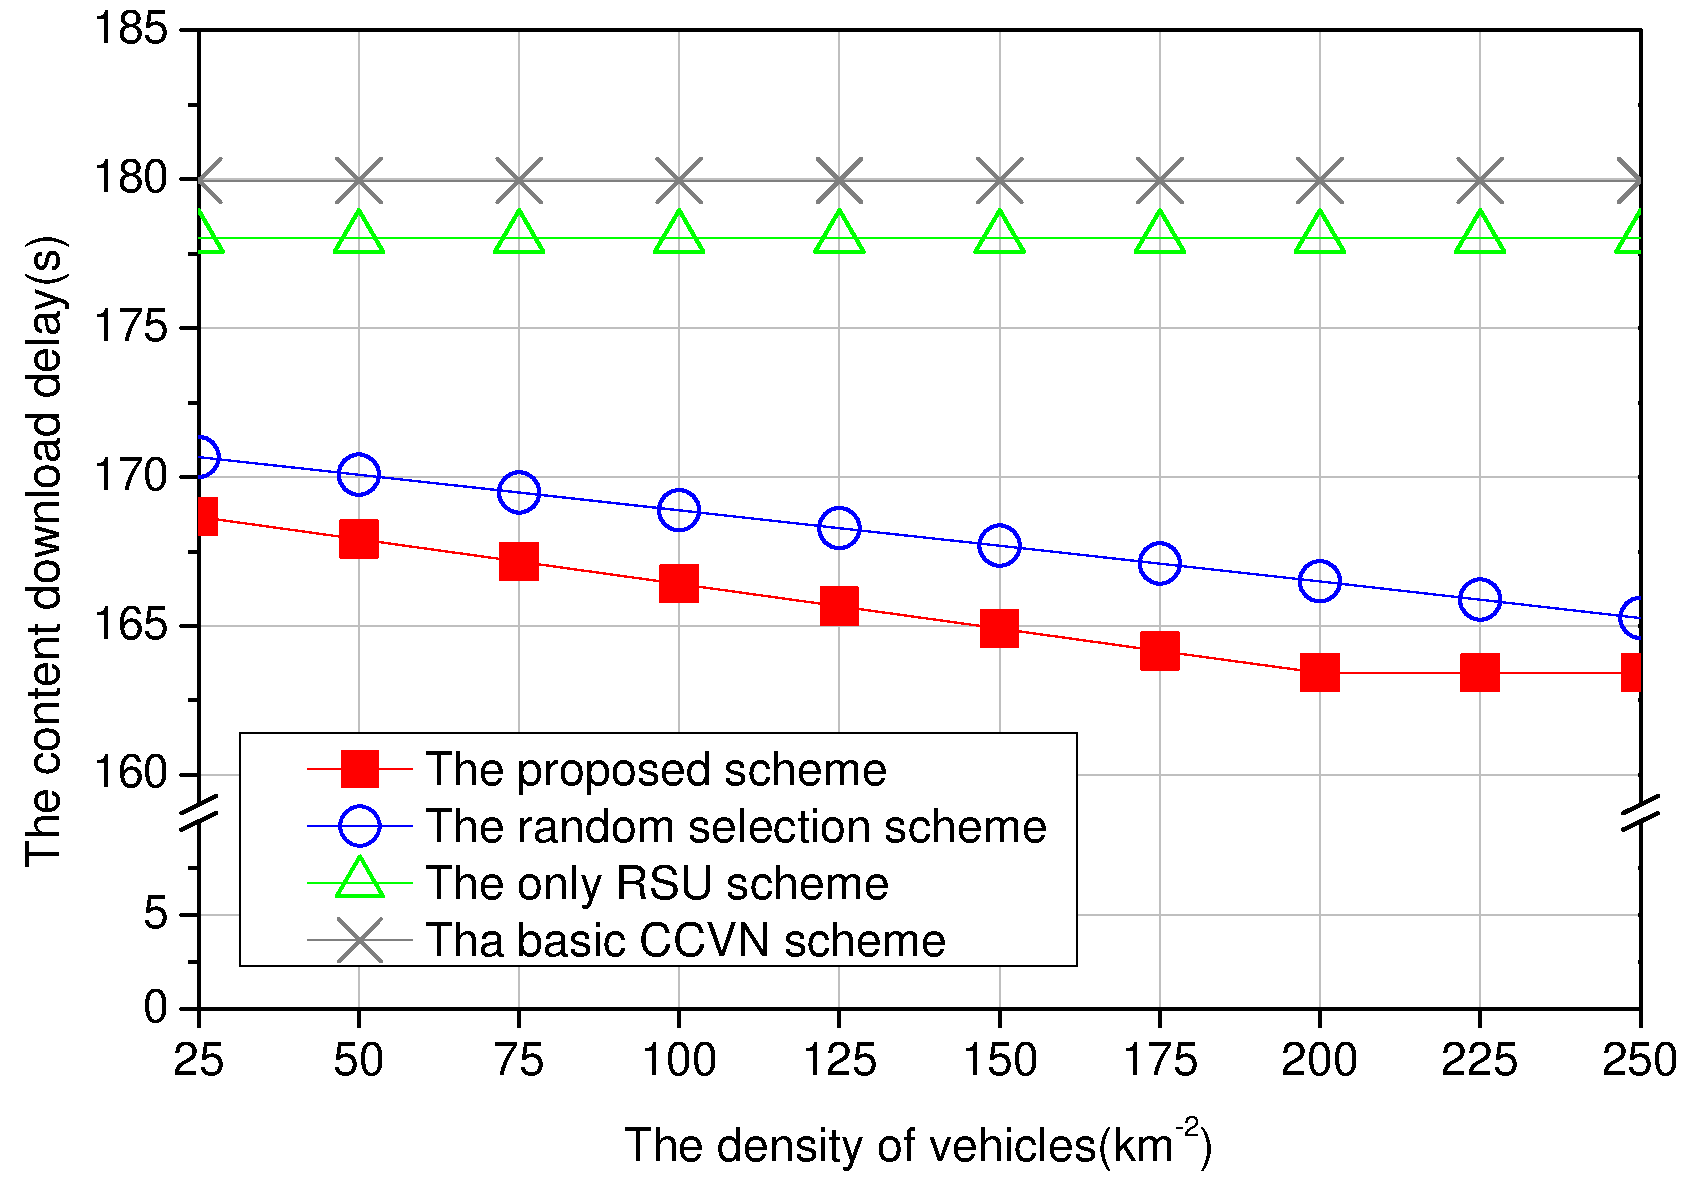
\includegraphics[width=0.48\textwidth]{./graph/D Delay.pdf}}
    \subfigure[]{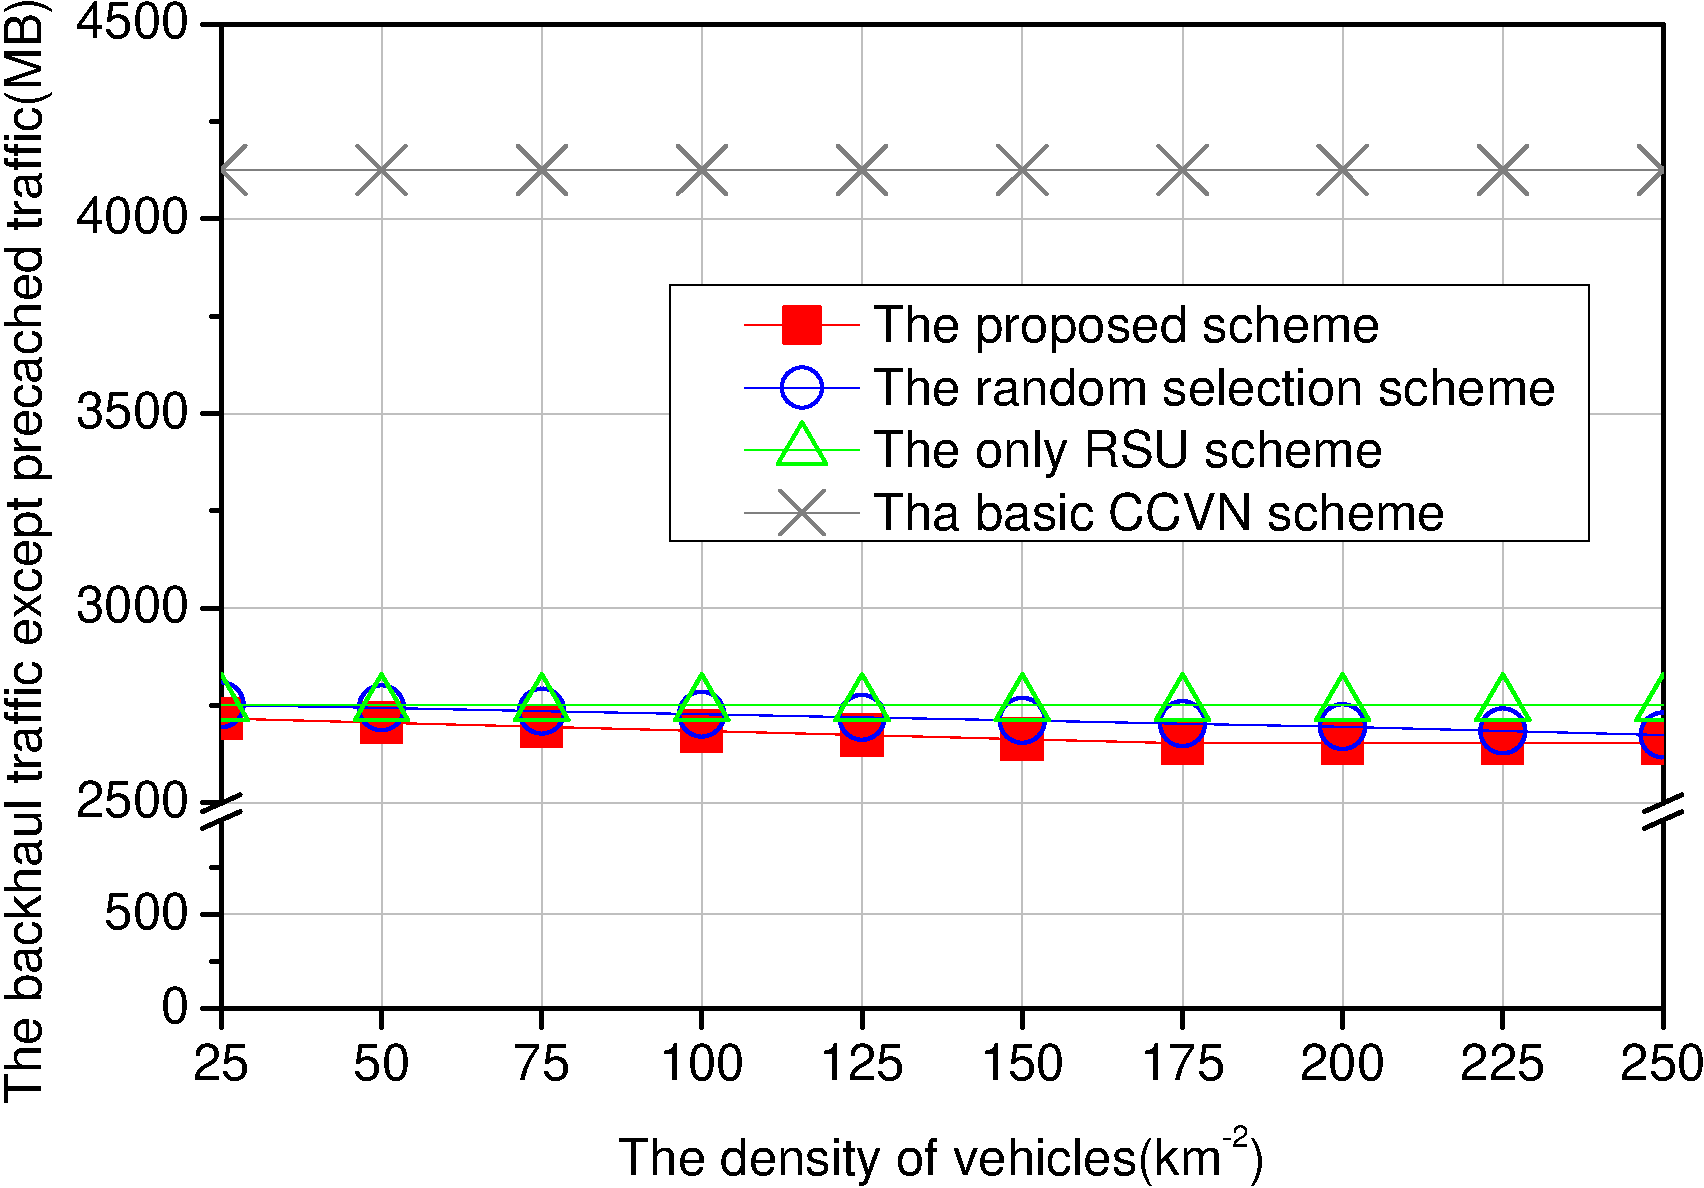
\includegraphics[width=0.48\textwidth]{graph/D Traffic.pdf}}\\
    \subfigure[]{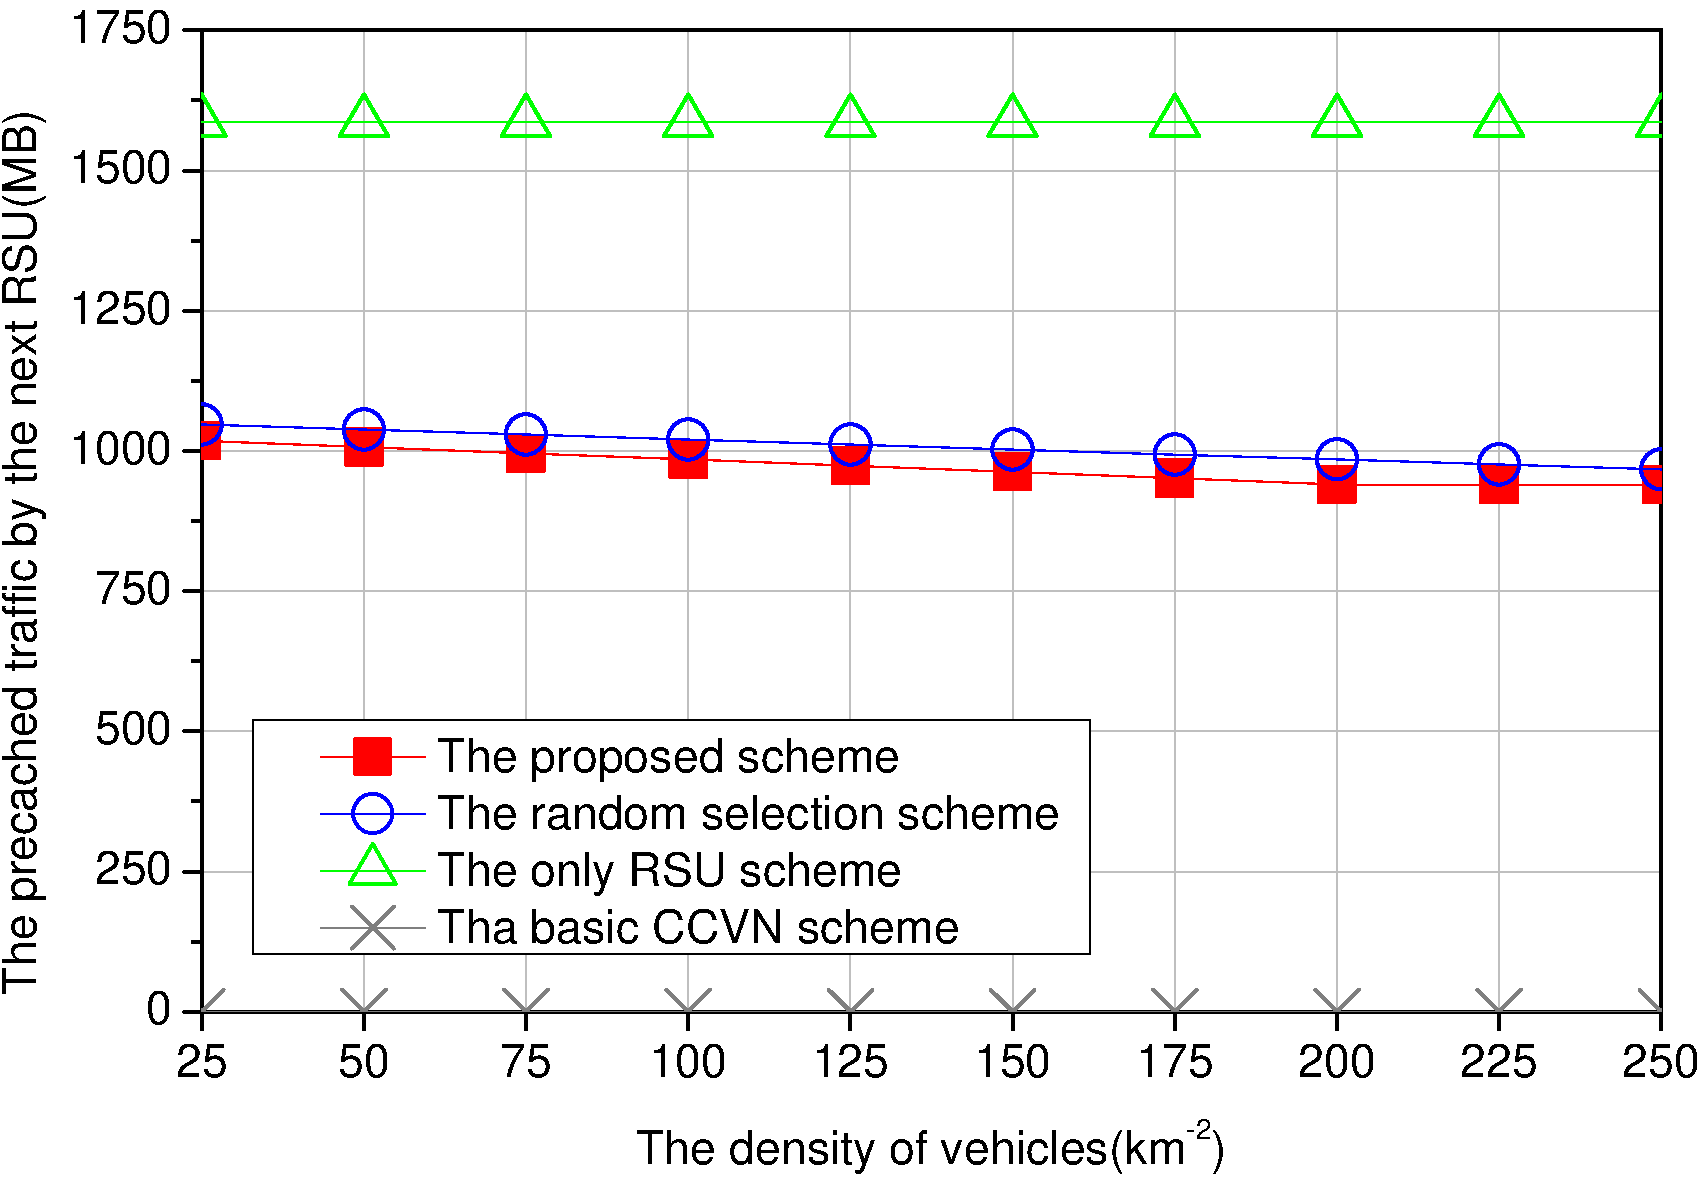
\includegraphics[width=0.48\textwidth]{graph/D Precache.pdf}}
    \subfigure[]{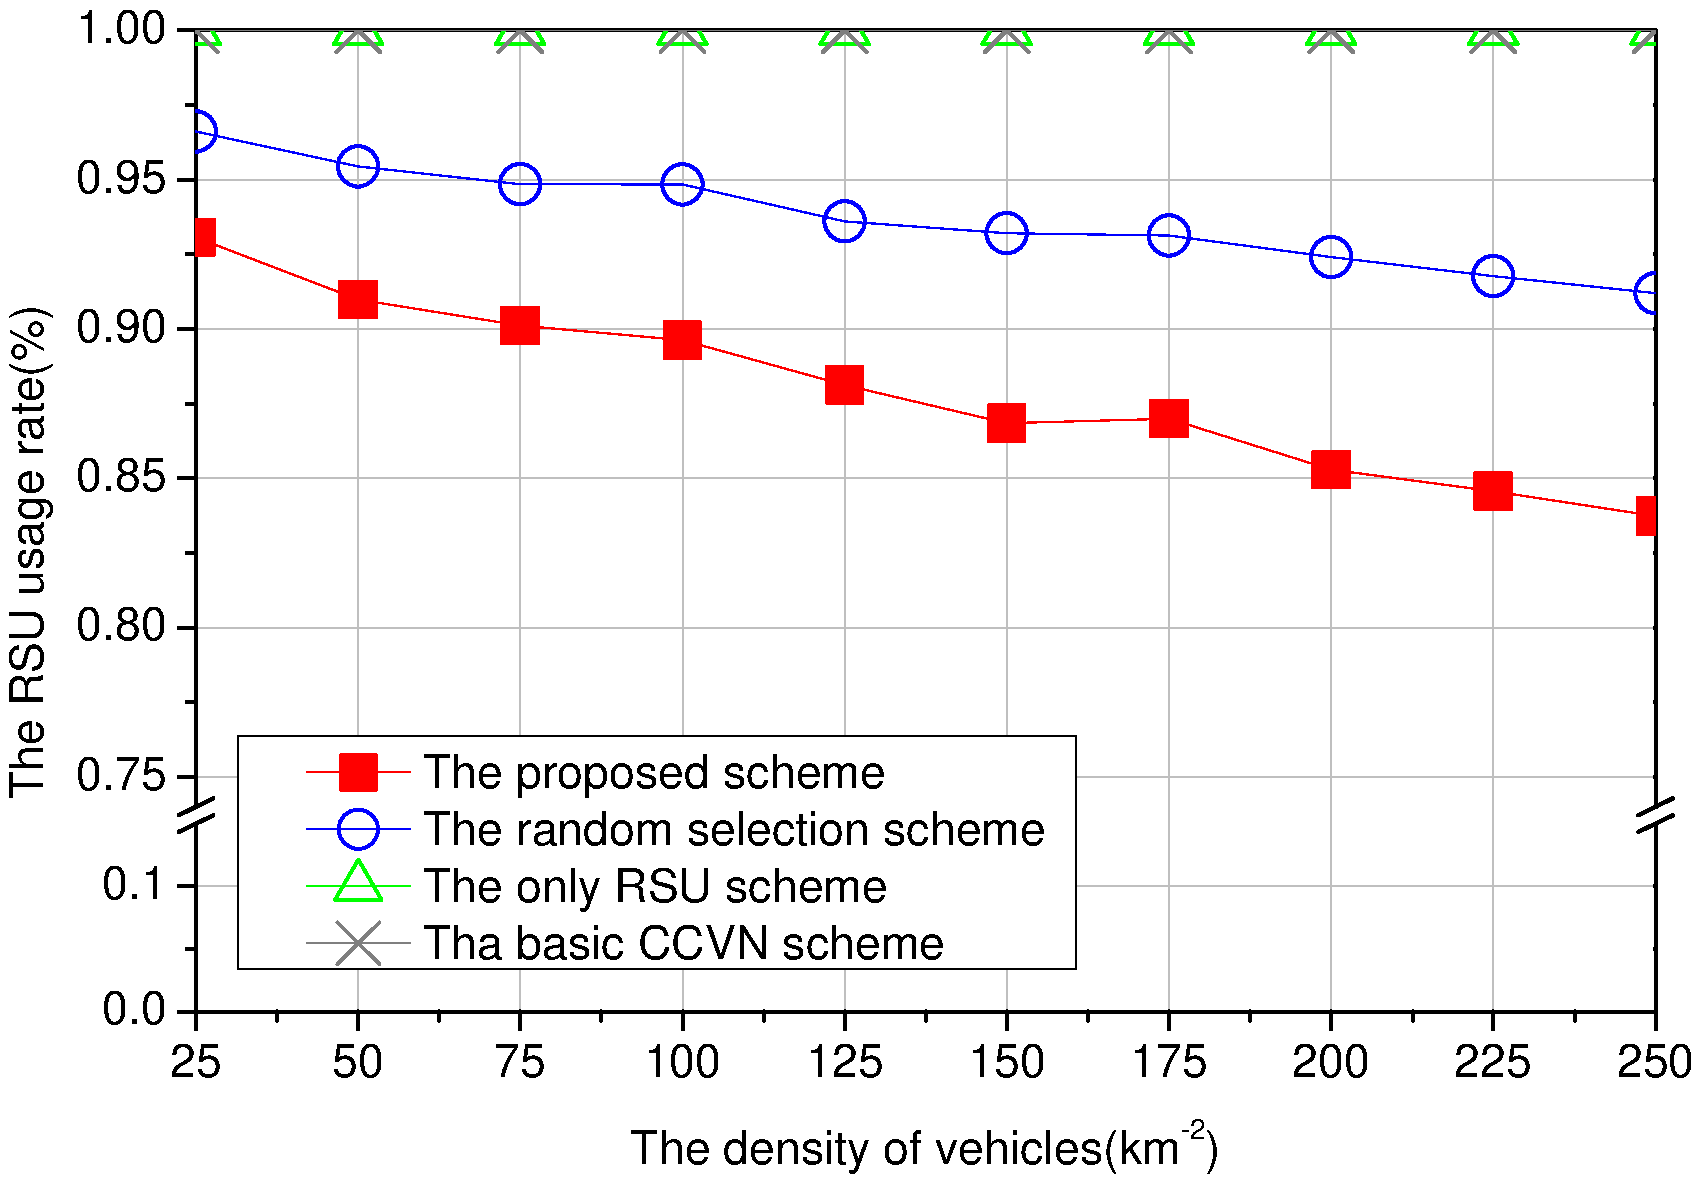
\includegraphics[width=0.48\textwidth]{graph/D RSU use.pdf}}
    \caption{\hl{Simulation} %MDPI: Please change the hyphen (-) into minus sign ($-$, "U+2212"). e.g., "-2" should be "$-$2".
 results for different densities of vehicles: (\textbf{a}) the content download delay, (\textbf{b})~the backhaul traffic except precached traffic, (\textbf{c}) the precached traffic by next RSU and (\textbf{d}) the RSU usage~rate.}
    \label{fig:a}
\end{figure}


In Figure \ref{fig:a}b, we evaluate the effect of vehicle density on the consumed backhaul traffic, except for precached traffic. The basic CCVN scheme consumes the resources of the links between the current RSU and the content server because it takes the requested content from the content server and provides it to ${V}_{req}$. Therefore, the performance is severely affected by the number of hops in terms of transmission speed. Only the RSU scheme performed better than the basic CCVN scheme because it precaches the content in the next RSU. However, these two schemes are not affected by vehicle density. The random selection scheme has improved performance because more relaying vehicles are available when the density of the vehicles is high. The proposed scheme exhibits the best performance because it can select the optimized relaying vehicles. Because the area between the current and next RSU is limited, the performance of the proposed scheme converges when there is a sufficient number of candidates.

Figure \ref{fig:a}c shows the precaching traffic according to the vehicle density. In the proposed scheme, a higher density of vehicles allows the selection of more optimal relaying vehicles, thereby reducing the size of the content that the next RSU should precache. This leads to a reduction in precaching traffic. In the random selection scheme, a lower density of vehicles increases the probability of using the worst or no candidate for the relaying vehicles; therefore, a larger amount of content should be precached at the next RSU. However, the RSU scheme is not affected by vehicle density. Furthermore, as the basic CCVN scheme does not use precaching, there is no precaching traffic.

Figure \ref{fig:a}d shows the percentage of RSUs used to provide content according to the density of the vehicle. The basic CCVN and RSU schemes depend only on RSUs for content delivery because they do not use vehicles as relay nodes. The random selection scheme improves performance because the probability of selecting a better relaying vehicle at a higher density of vehicles increases. The proposed scheme effectively reduced the rate of dependence on RSUs because optimal relaying vehicles can be selected at a higher density of vehicles.



In Figure \ref{fig:b}, we evaluated the performance according to the density of the RSUs by adjusting the distance between the RSUs. Figure \ref{fig:b}a depicts the effect of the density of RSUs on the content download delay. In the basic CCVN scheme and the only RSU scheme, because vehicles are not used as relay nodes, the content download delay increases as the time that ${V}_{req}$ reaches the next RSU increases when the distance between RSUs is long. Additionally, because the basic CCVN scheme is inefficient in terms of the transmission rate, it has the longest delay. However, in the proposed scheme and the random selection scheme, because a sufficient number of relaying vehicles are used to provide the content for ${V}_{req}$ outside the RSUs’ communication range, it is less affected by the density of RSUs. Because the random selection scheme does not select the optimal relaying vehicles, ${V}_{req}$ must receive the remaining portion of the content from the next RSU. Hence, on average, the proposed scheme has less delay than the random-selection scheme.


\begin{figure}[H]
    \subfigure[]{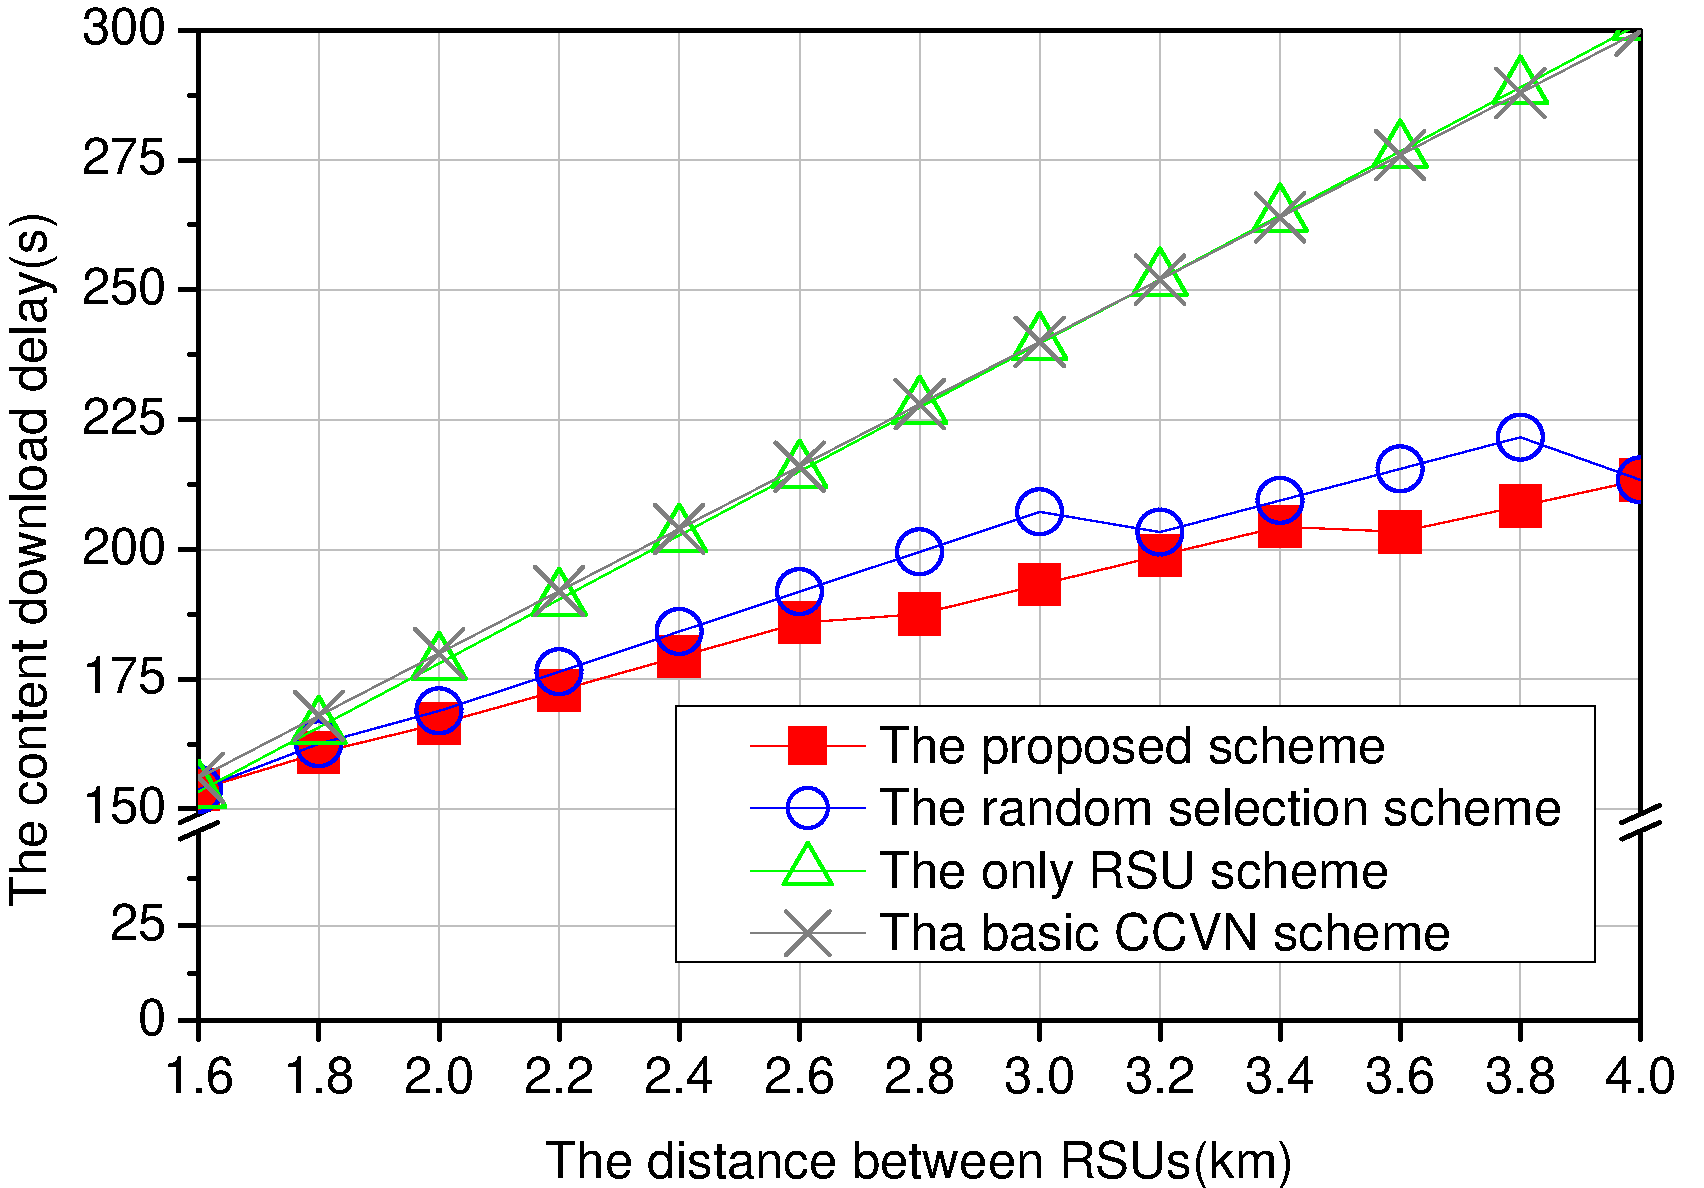
\includegraphics[width=0.48\textwidth]{./graph/R Delay.pdf}}
    \subfigure[]{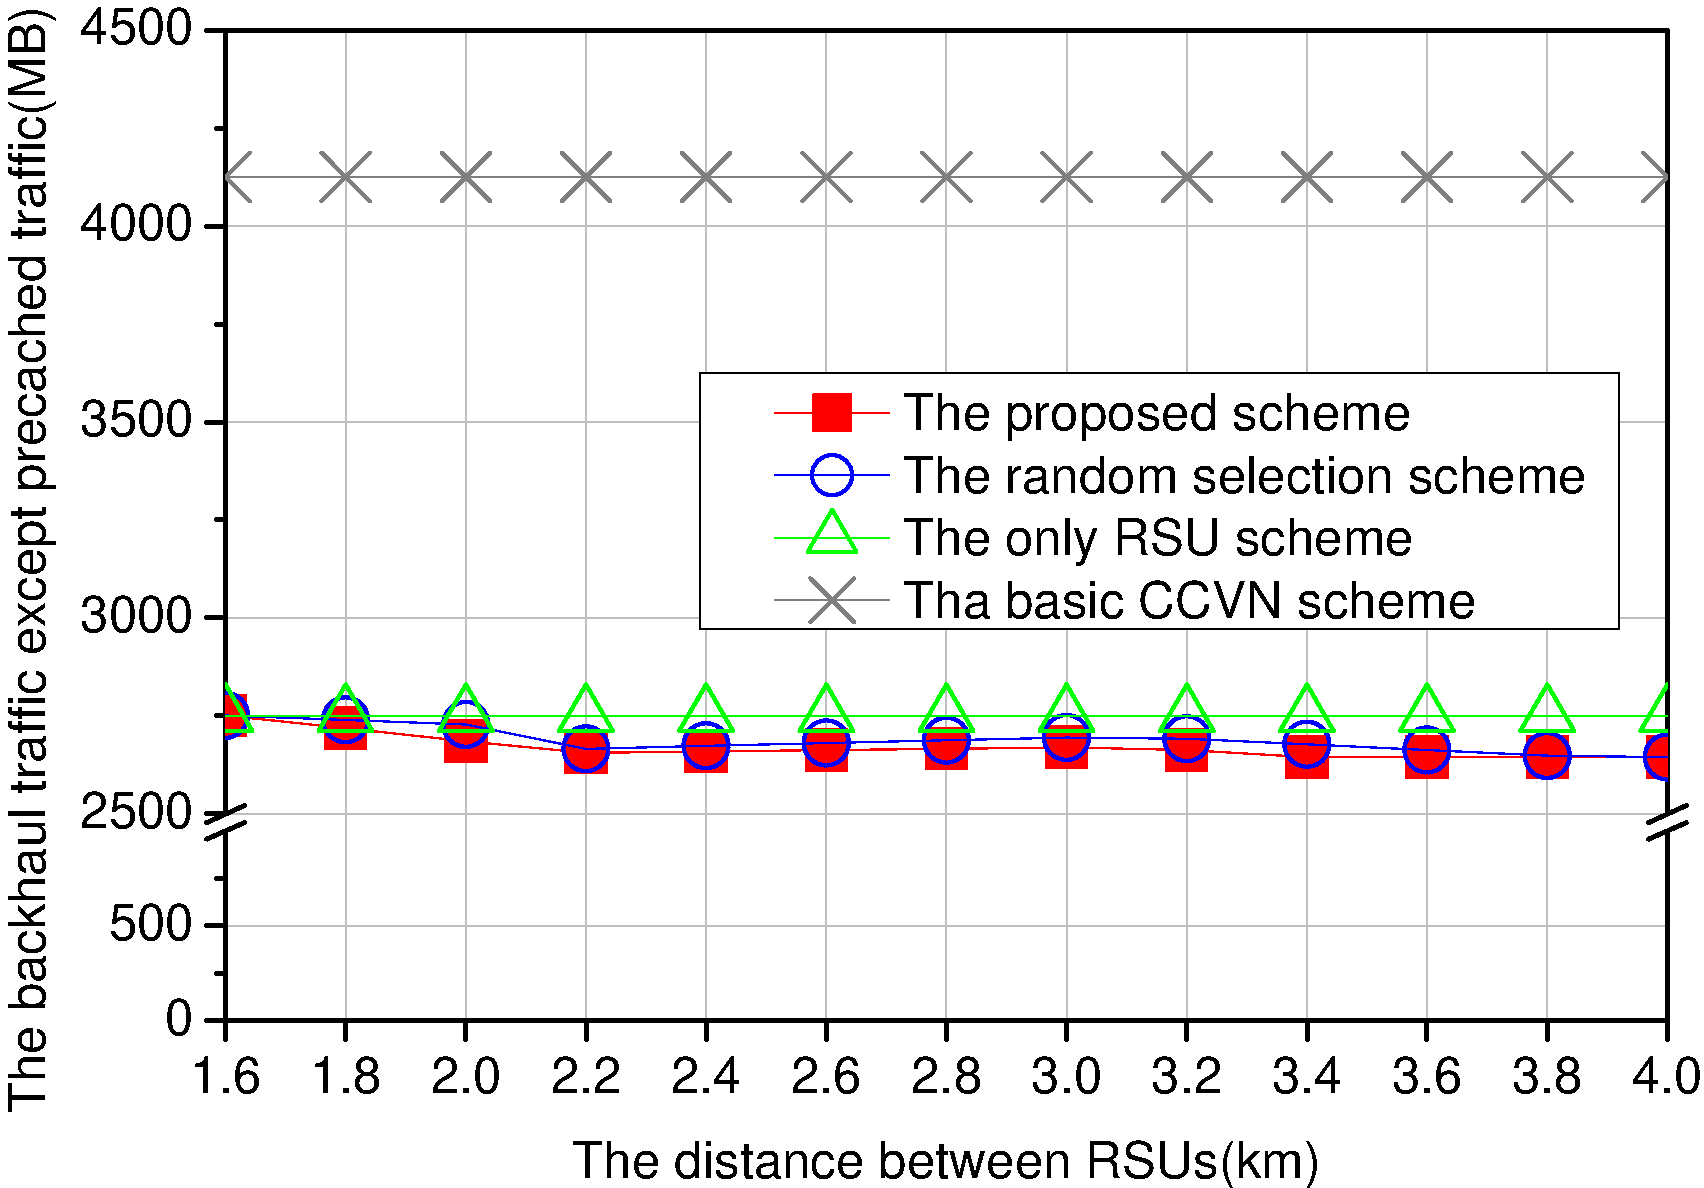
\includegraphics[width=0.48\textwidth]{graph/R Traffic.pdf}}\\
    \subfigure[]{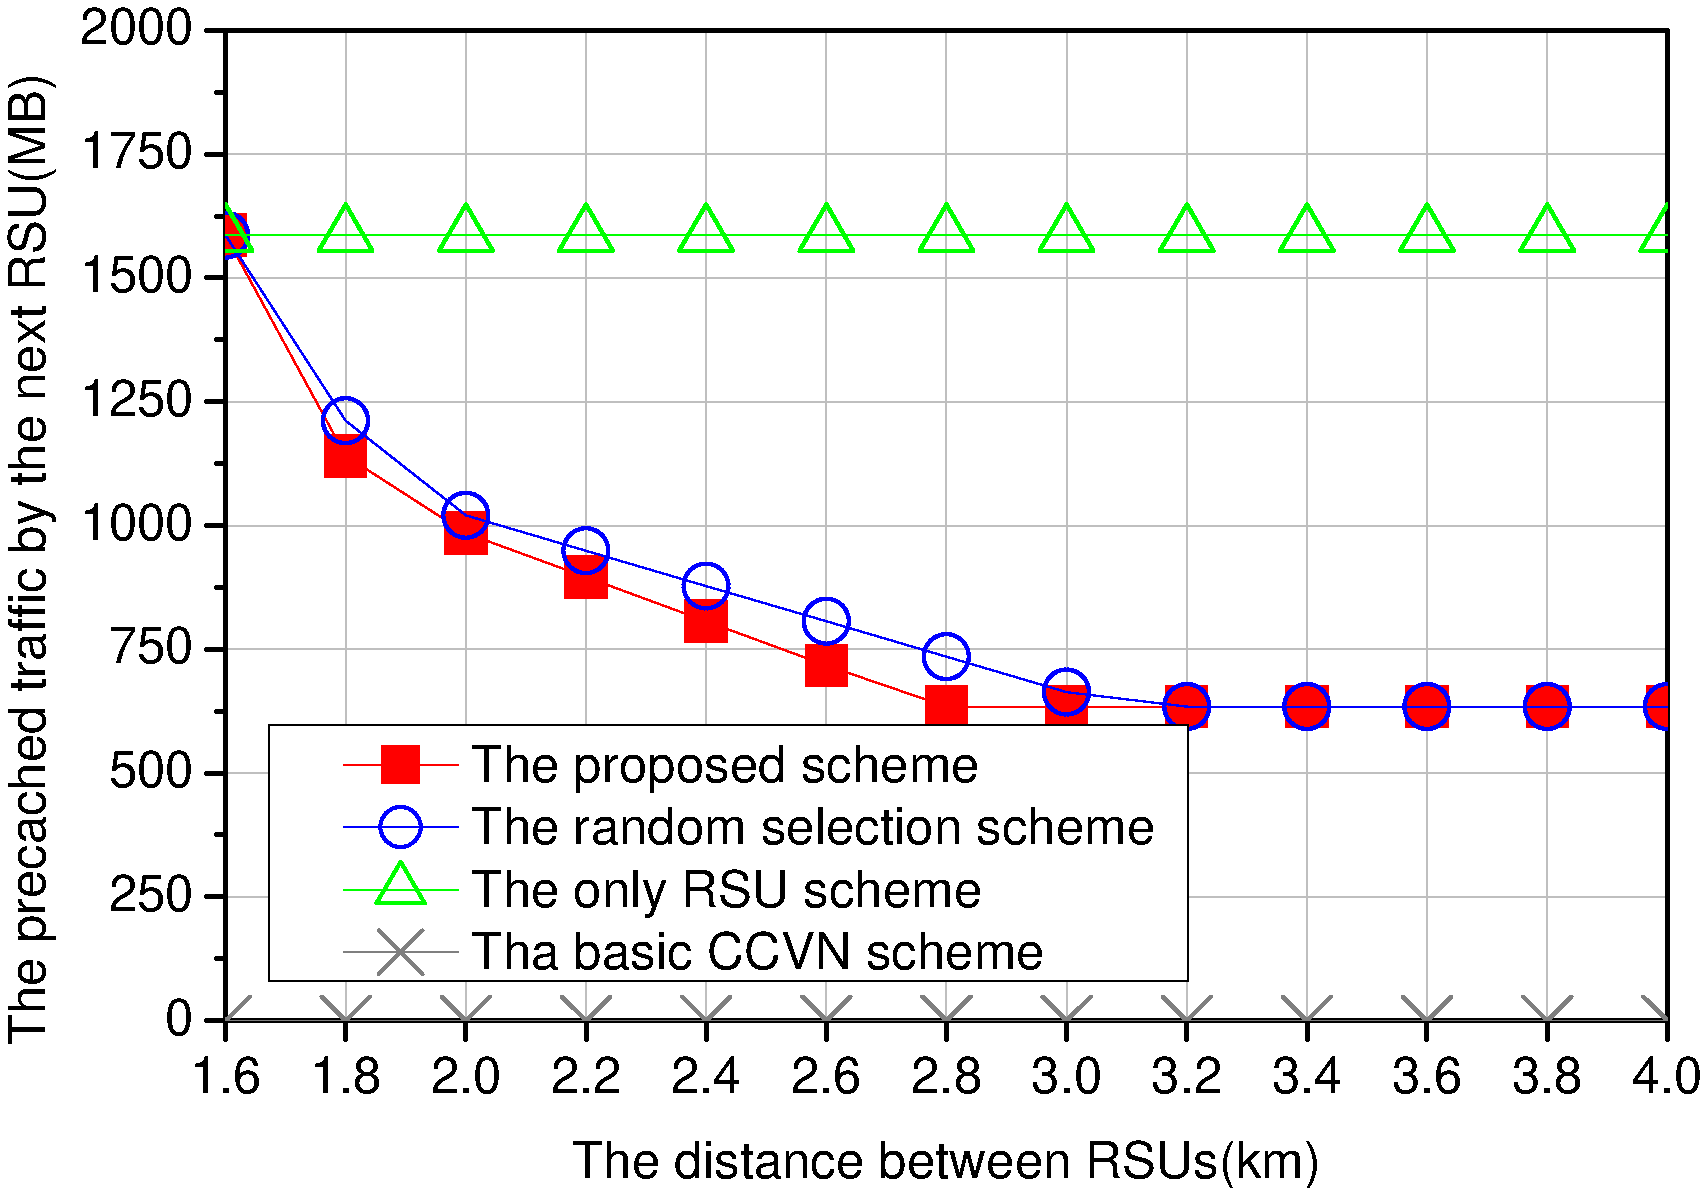
\includegraphics[width=0.48\textwidth]{graph/R Precache.pdf}}
    \subfigure[]{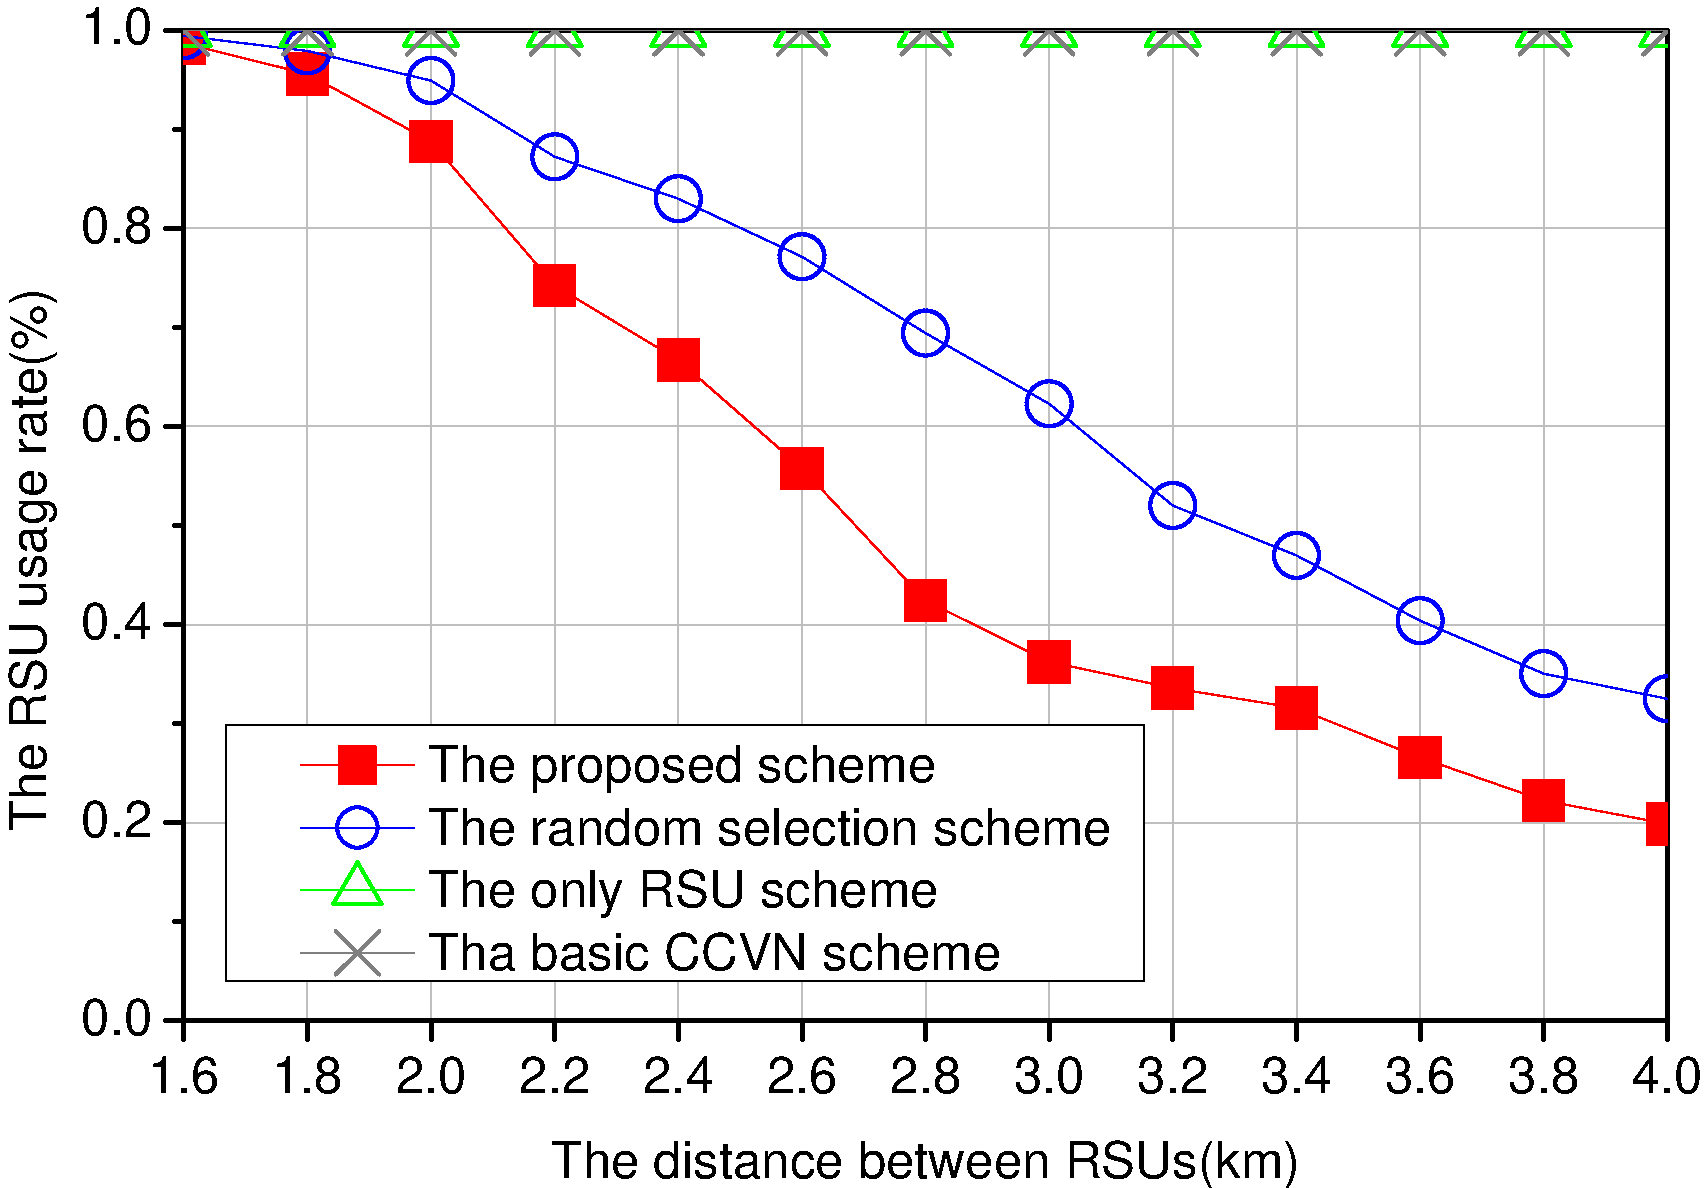
\includegraphics[width=0.48\textwidth]{graph/R RSU use.pdf}}
    \caption{Simulation results for different distances between RSUs: (\textbf{a}) the content download delay, (\textbf{b}) the backhaul traffic except precached traffic, (\textbf{c}) the precached traffic by next RSU and (\textbf{d}) the RSU usage rate.}
    \label{fig:b}
\end{figure}


Figure \ref{fig:b}b shows the effect of the density of RSUs on traffic that relays the content directly from the content server to ${V}_{req}$, except for the traffic consumed by RSUs for precaching. The relayed traffic consumed by the RSU to relay content directly from the content server to ${V}_{req}$ has a slow transmission rate, consuming more links than the RSU directly delivering the precached content to the vehicle. Because the content cannot be precached in the first RSU, all schemes relayed traffic from the content server. In particular, the basic CCVN scheme provides the entire content by relaying it from the content server to the vehicle as it does not use precaching. In the case of the basic CCVN scheme and the only RSU scheme, the backhaul traffic generated is not related to the distance between RSUs, because the content can only be provided within the RSU communication range. However, if the next RSU is far-off, the RSU consumes less traffic to relay directly from the content server to ${V}_{req}$ because the proposed scheme and random selection scheme precache most of the content on the relaying vehicles. Because the proposed scheme prepares more content for optimized relaying vehicles, the relayed traffic is the least.


Figure \ref{fig:b}c presents the traffic consumed by RSUs to precache the content according to the density of the RSUs. The basic CCVN scheme does not use precaching. The RSU scheme is not affected by the distance between the RSUs because ${V}_{req}$ only receives the content within the RSU communication range. However, in the proposed and random selection schemes, the traffic consumed by the precache to be borne by RSUs is reduced because ${V}_{req}$ receives most of the content via V2V communication, except for the first RSU. With the optimal candidate selection algorithm, the proposed scheme significantly relieves the burden of the next RSUs.

In Figure \ref{fig:b}d, we present the proposed scheme and the random selection scheme for mitigating the burden on the RSU. Because these two schemes provide almost all of the content to ${V}_{req}$ via V2V communication if the distance between RSUs is large, this reduces the amount of content that the RSUs have to support. Furthermore, the proposed scheme is more effective than other schemes because it uses a larger number of available relaying~vehicles.


\subsection{Performance Based on Characteristics of Requester Vehicles} \label{sec5.3}



In Figure \ref{fig:c}, we evaluate the performance of the proposed scheme according to various sizes of content because the user can request various types of content. Figure \ref{fig:c}a shows that the content download delay is proportional to the size of the requested content. Because the transmission rate is limited, the delay in receiving the entire content increases in all schemes when the size of the requested content is large. In the basic CCVN scheme, because the entire requested content is relayed to ${V}_{req}$ from the content server, it is the most inefficient in terms of transmission rate. Therefore, this scheme has the greatest delay in downloading the content. Because only the RSU scheme receives the requested content from the RSU, additional delays are accumulated as they move outside the RSUs’ communication range. However, the proposed scheme and the random selection scheme consumed less delay because they can provide the content when ${V}_{req}$ is not only in the RSUs’ communication range but also out of the range. The random selection scheme, which randomly selects relaying vehicles, is inefficient compared with the proposed scheme.

In Figure \ref{fig:c}b, we evaluate the impact of the increase in the size of the requested content on backhaul traffic. Because the backhaul link consumed increases proportionally to the number of hops between the content servers and the next RSUs, the traffic consumption is larger than the size of the requested content. All schemes, except the basic CCVN scheme, consumed the most backhaul traffic when the requested content was provided in the first RSU. In addition, in these schemes, additional traffic increases with the difference between the size of the precached content and the actual received content. Because the RSU scheme uses only the RSU, it consumes more backhaul traffic than the two schemes using relaying vehicles. On the other hand, the basic CCVN scheme receives all chunks of content from the content server through relaying. Therefore, it consumes the most relayed traffic.

Figure \ref{fig:c}c shows the relationship between the size of the requested content and precaching traffic. To precache the content, the next RSU takes chunks of the content from the content server. Hence, the consumed traffic relies on the number of hops between the RSU and the content server. The basic CCVN scheme does not use a precache. In the case of the RSU scheme, most of the traffic is consumed because all chunks of the content, except the portion of the received content from the first RSU, are provided to ${V}_{req}$ by the next RSUs precaching the content. Because the other two schemes use relaying vehicles to precache the content, the traffic that RSUs are burdened with precaching the content is reduced.

Figure \ref{fig:c}d shows the burden of RSUs according to the size of the requested content. Because the proposed scheme selects optimized relaying vehicles, the RSUs’ burden is reduced the most. In comparison, the random selection scheme that selects any relaying vehicle cannot guarantee that ${V}_{req}$ is served with maximum efficiency outside the RSUs’ communication range. Thus, there is a greater burden on the RSUs than in the proposed scheme. The size of the requested content that can be provided is limited because ${V}_{req}$ has available time owing to the mobility of the vehicle outside of the RSUs’ communication range. Therefore, a sufficient size of the requested content converges to alleviate the burden of the RSUs.


\begin{figure}[H]
    \subfigure[]{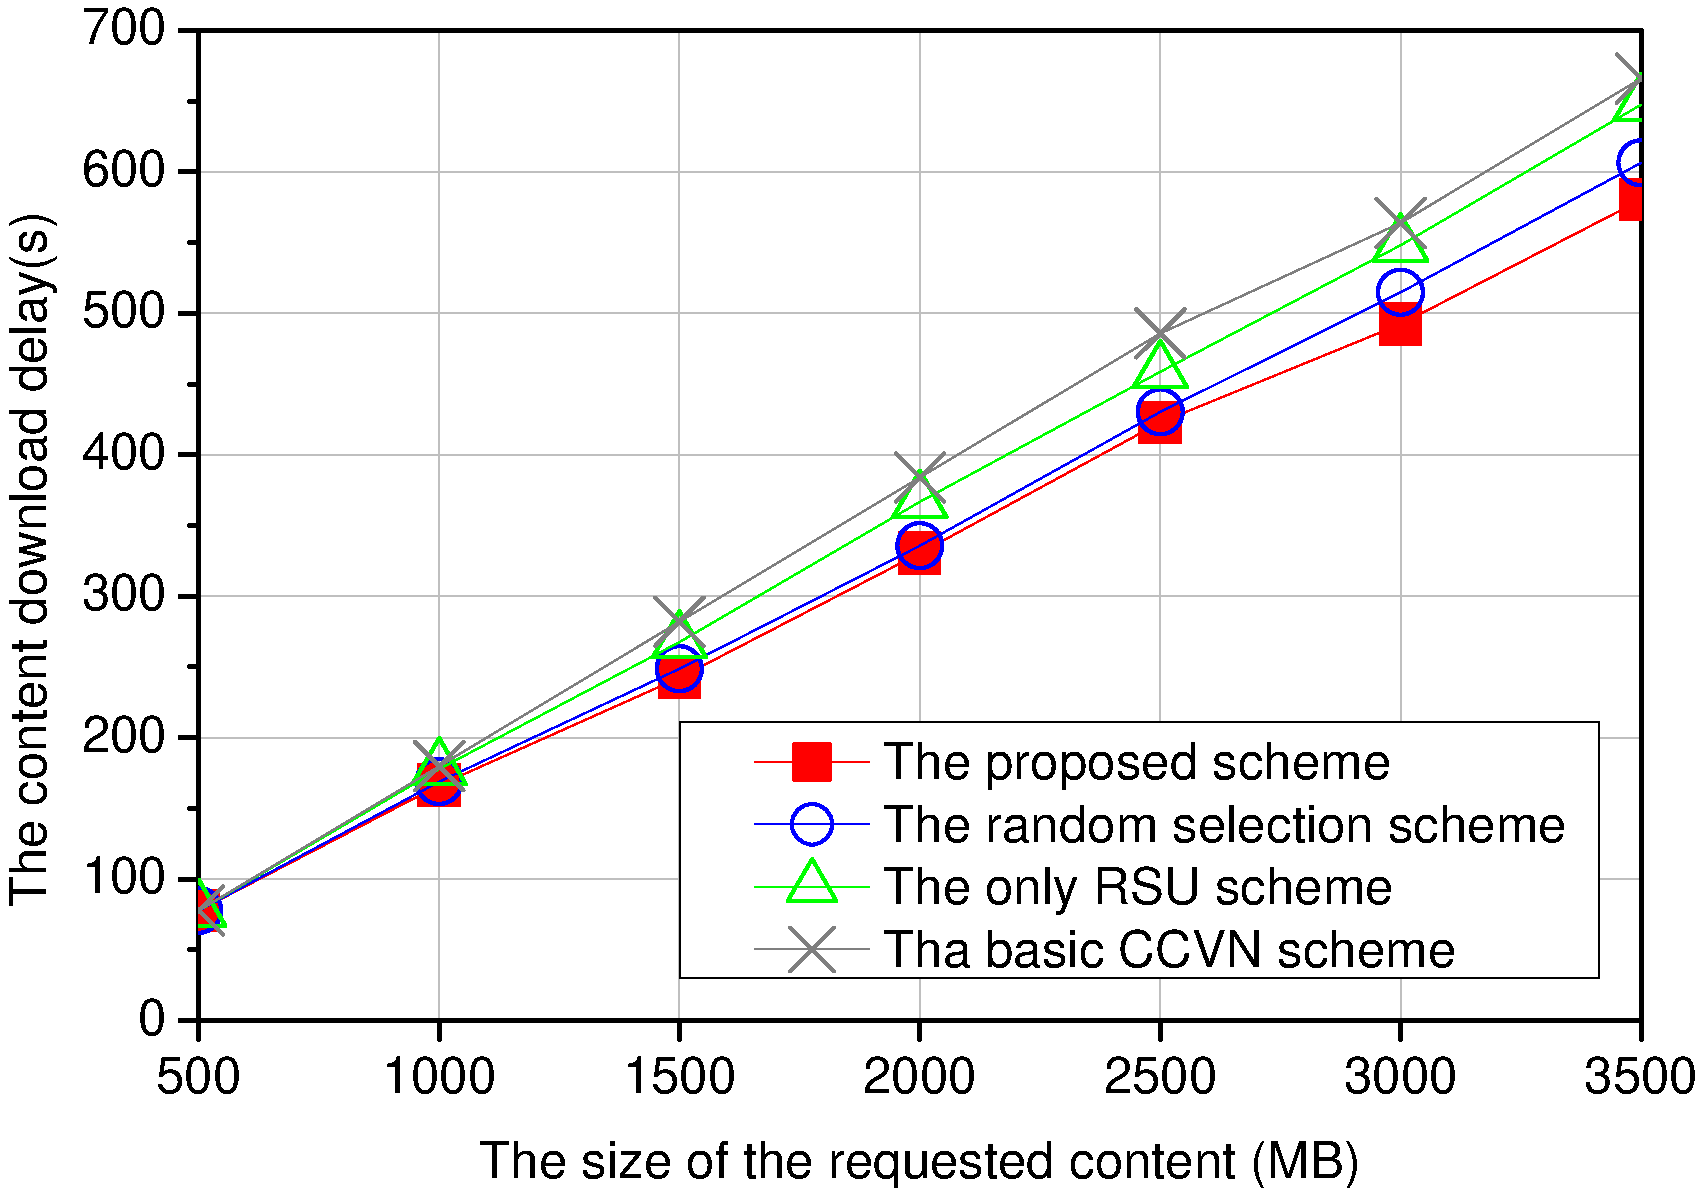
\includegraphics[width=0.48\textwidth]{./graph/C Delay.pdf}}
    \subfigure[]{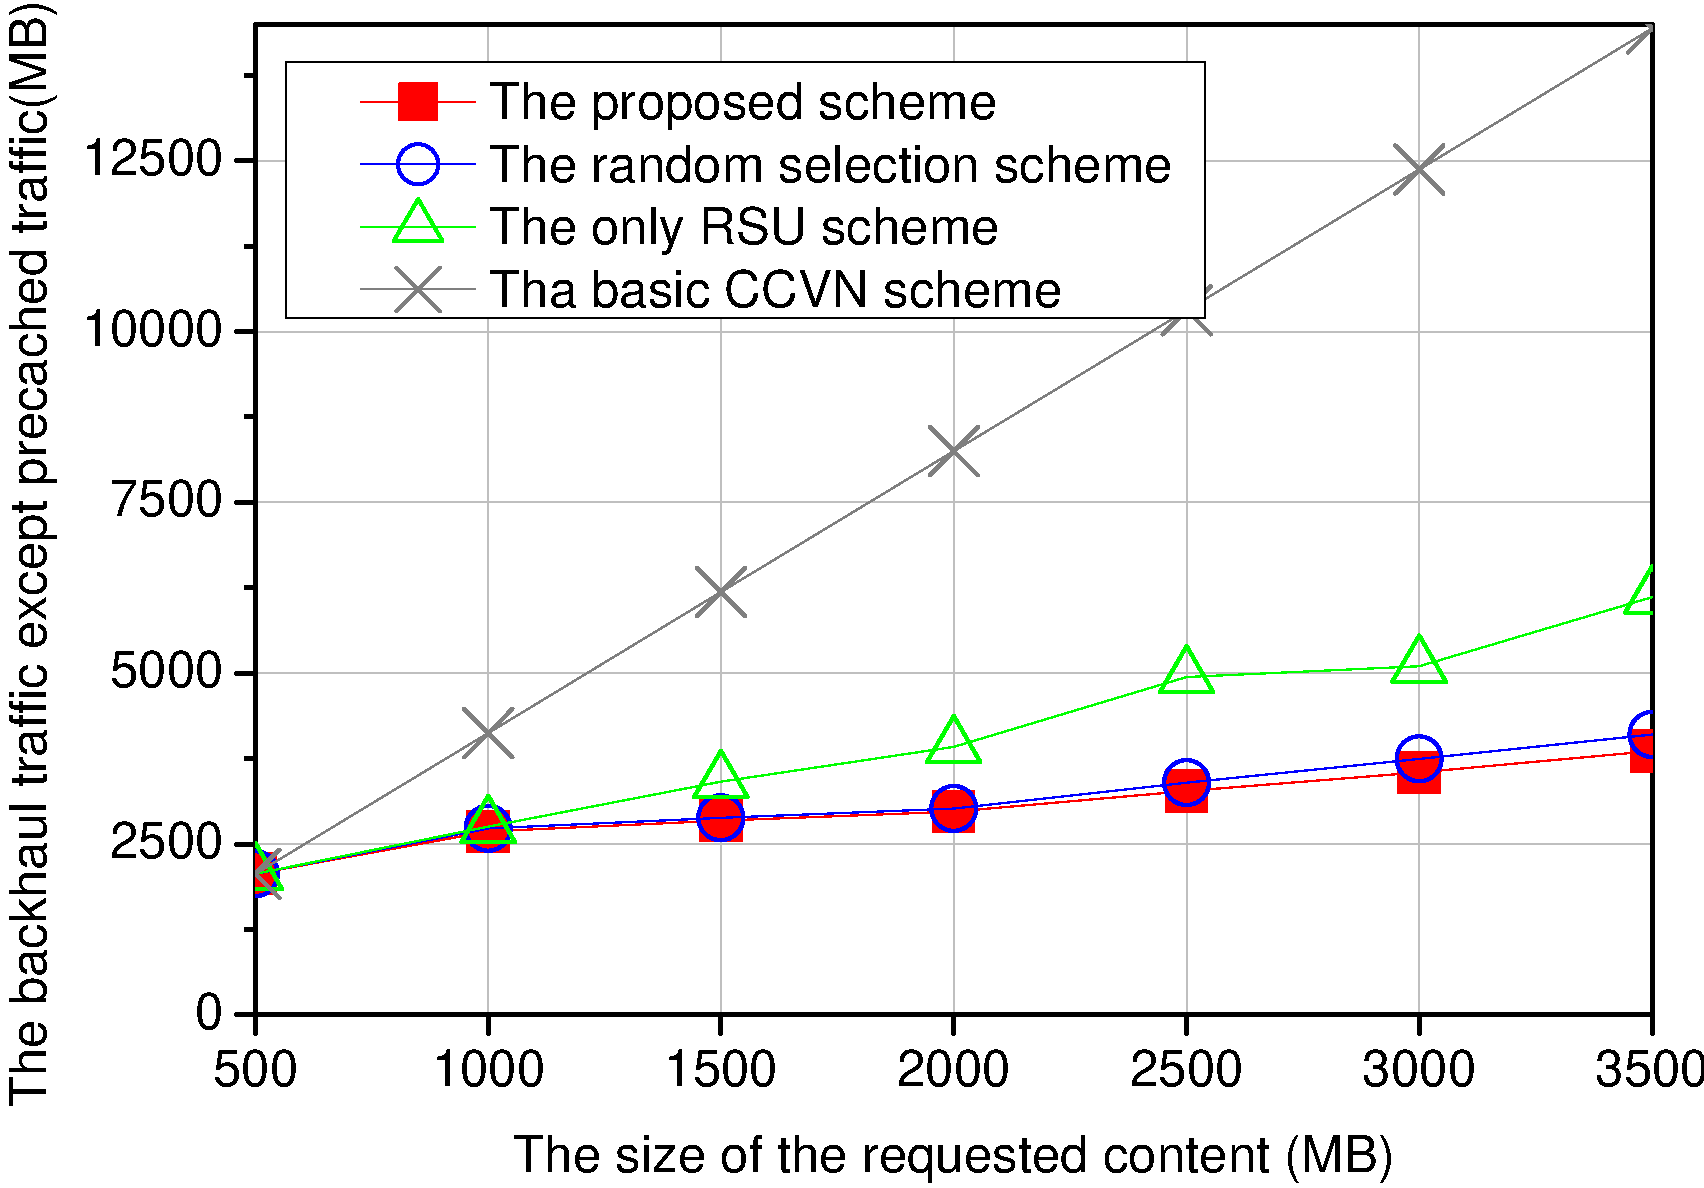
\includegraphics[width=0.48\textwidth]{graph/C Traffic.pdf}}\\
    \subfigure[]{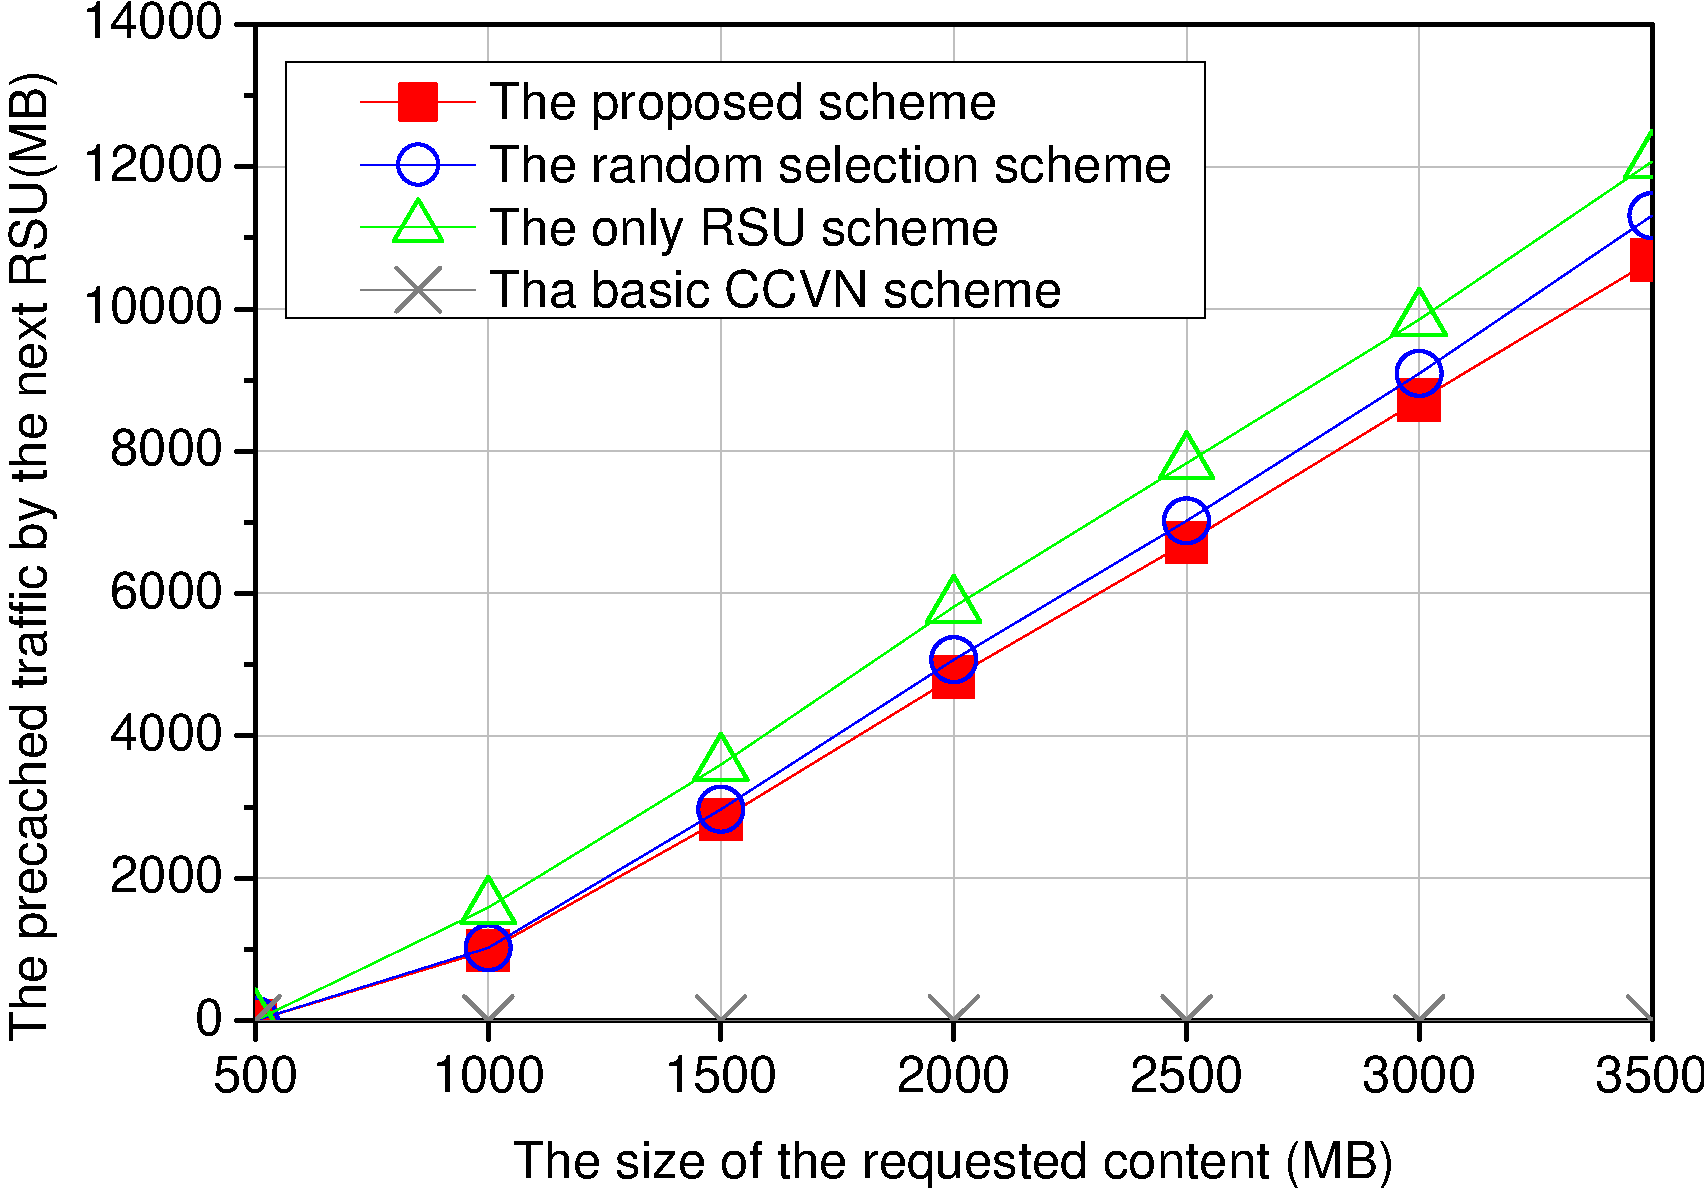
\includegraphics[width=0.48\textwidth]{graph/C Precache.pdf}}
    \subfigure[]{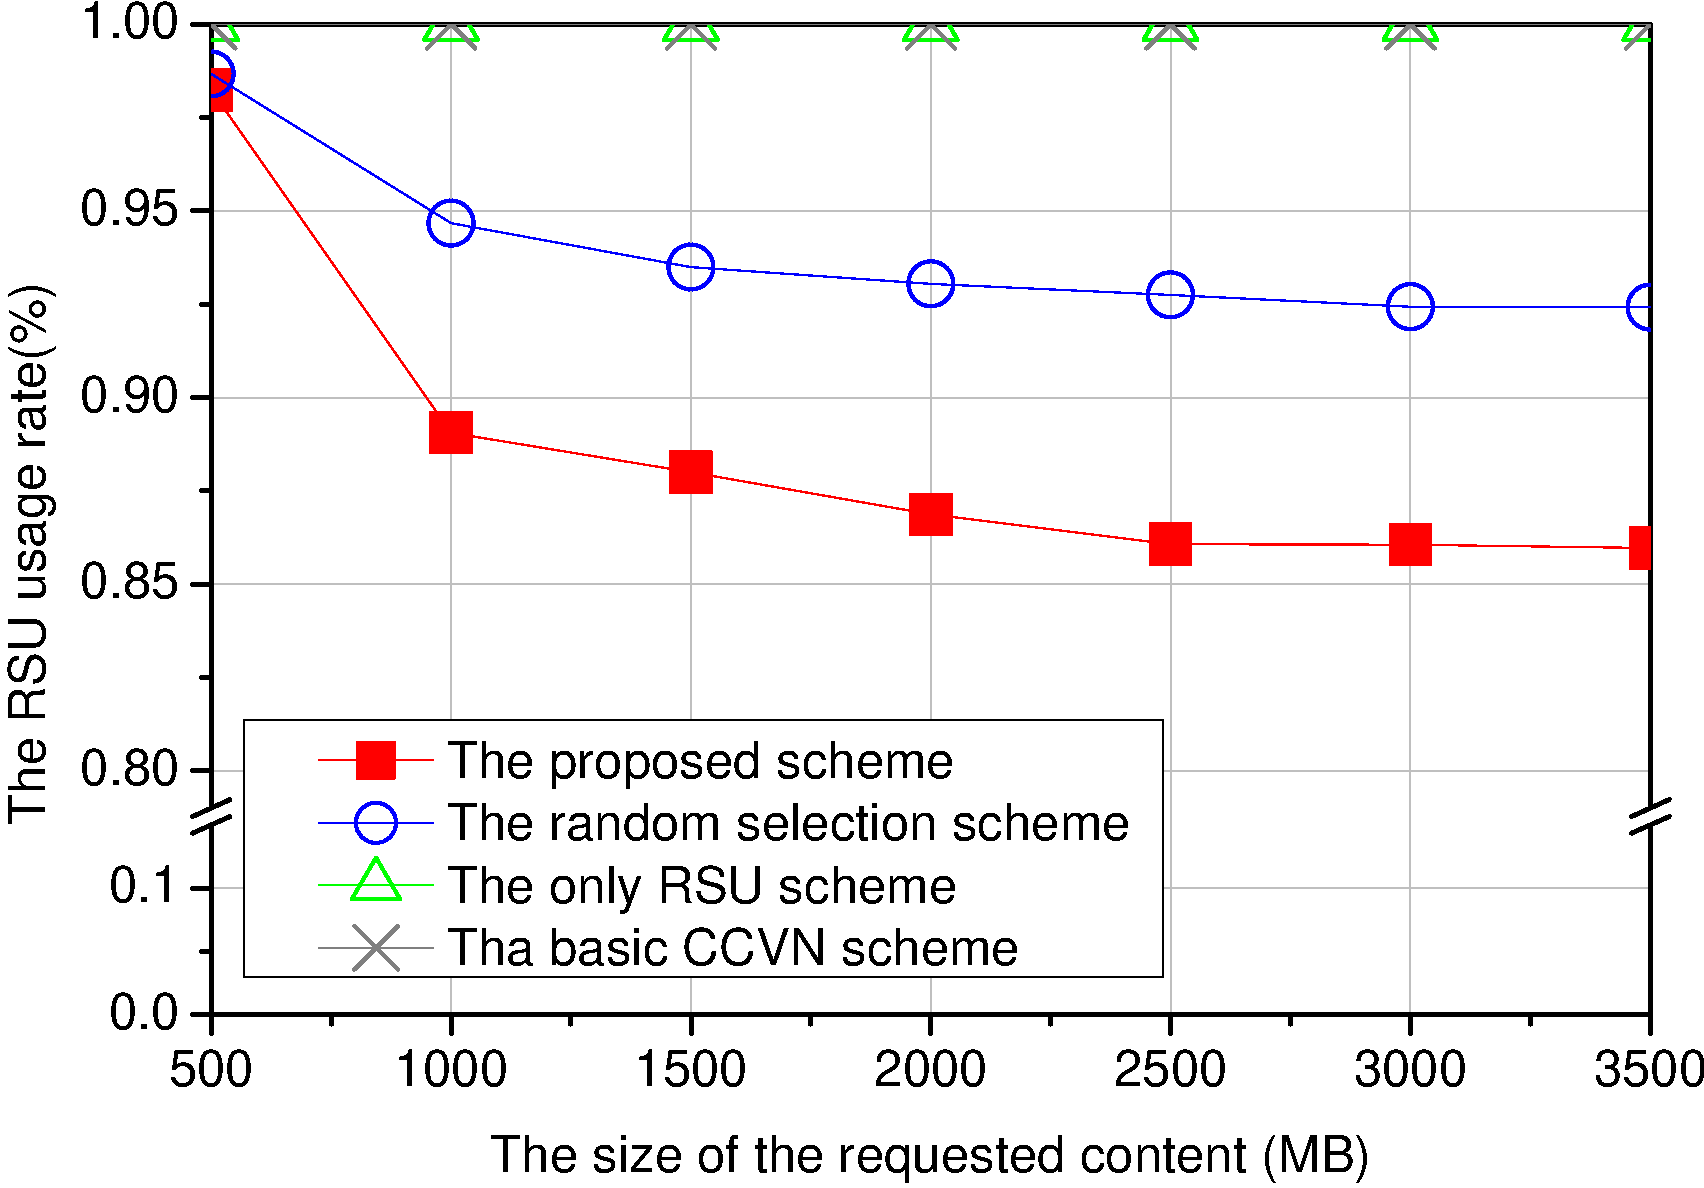
\includegraphics[width=0.48\textwidth]{graph/C RSU use.pdf}}
    \caption{Simulation %MDPI: Please use commas to separate thousands for numbers with five or more digits (not for four digits) in the picture. e.g., "10000" should be "10,000"
 results for different sizes of the requested content : (\textbf{a}) the content download delay, (\textbf{b}) the backhaul traffic except precached traffic, (\textbf{c}) the precached traffic by next RSU and (\textbf{d})~the RSU usage rate.}
    \label{fig:c}
\end{figure}


In Figure \ref{fig:d}, we also evaluate the performance of various user characteristics. Figure \ref{fig:d}a shows the content download delay according to the speed of the vehicle. If the speed of the vehicle is low, the next RSU and ${V}_{rel}$ do not have to precache the content because ${V}_{req}$ has sufficient dwell time to receive the entire content from the content server in the first RSU. Otherwise, if the speed of the vehicle is high, the number of content chunks not received by the first RSU increases. Therefore, the content download delay is increased because ${V}_{req}$ requires time to reach the next RSU to receive the rest of the content. Subsequently, the delay continues to decrease because the time remaining in the outage zone decreases with increasing speed before additional RSUs are required. Because only the RSU scheme and the basic CCVN scheme that do not use the relaying vehicles are provided with content only through the RSU to ${V}_{req}$, the content download delay in both schemes depends more on the time ${V}_{req}$ required to reach the next RSU than in the other two schemes. %please verify
% 변동의 이유
The faster speed of the requester vehicle can decrease the download delay because it can reduce the time within the outage zone.
However, at some speed of the requester vehicle, the increased delay due to the decreased time that the requester vehicle can receive the requested content within the coverage of RSUs has more impact than the decreased delay by reduced time within the outage zone.
That is why the content download delay of the two schemes significantly fluctuated.
The RSU scheme has a shorter delay than the basic CCVN scheme because the next RSU precaches the content. In the random selection scheme, the delay is shorter because it is provided by the randomly selected ${V}_{rel}$ in the outage zone. The proposed scheme has the least delay because it selects the optimal ${V}_{rel}$.

\begin{figure}[H]
    \subfigure[]{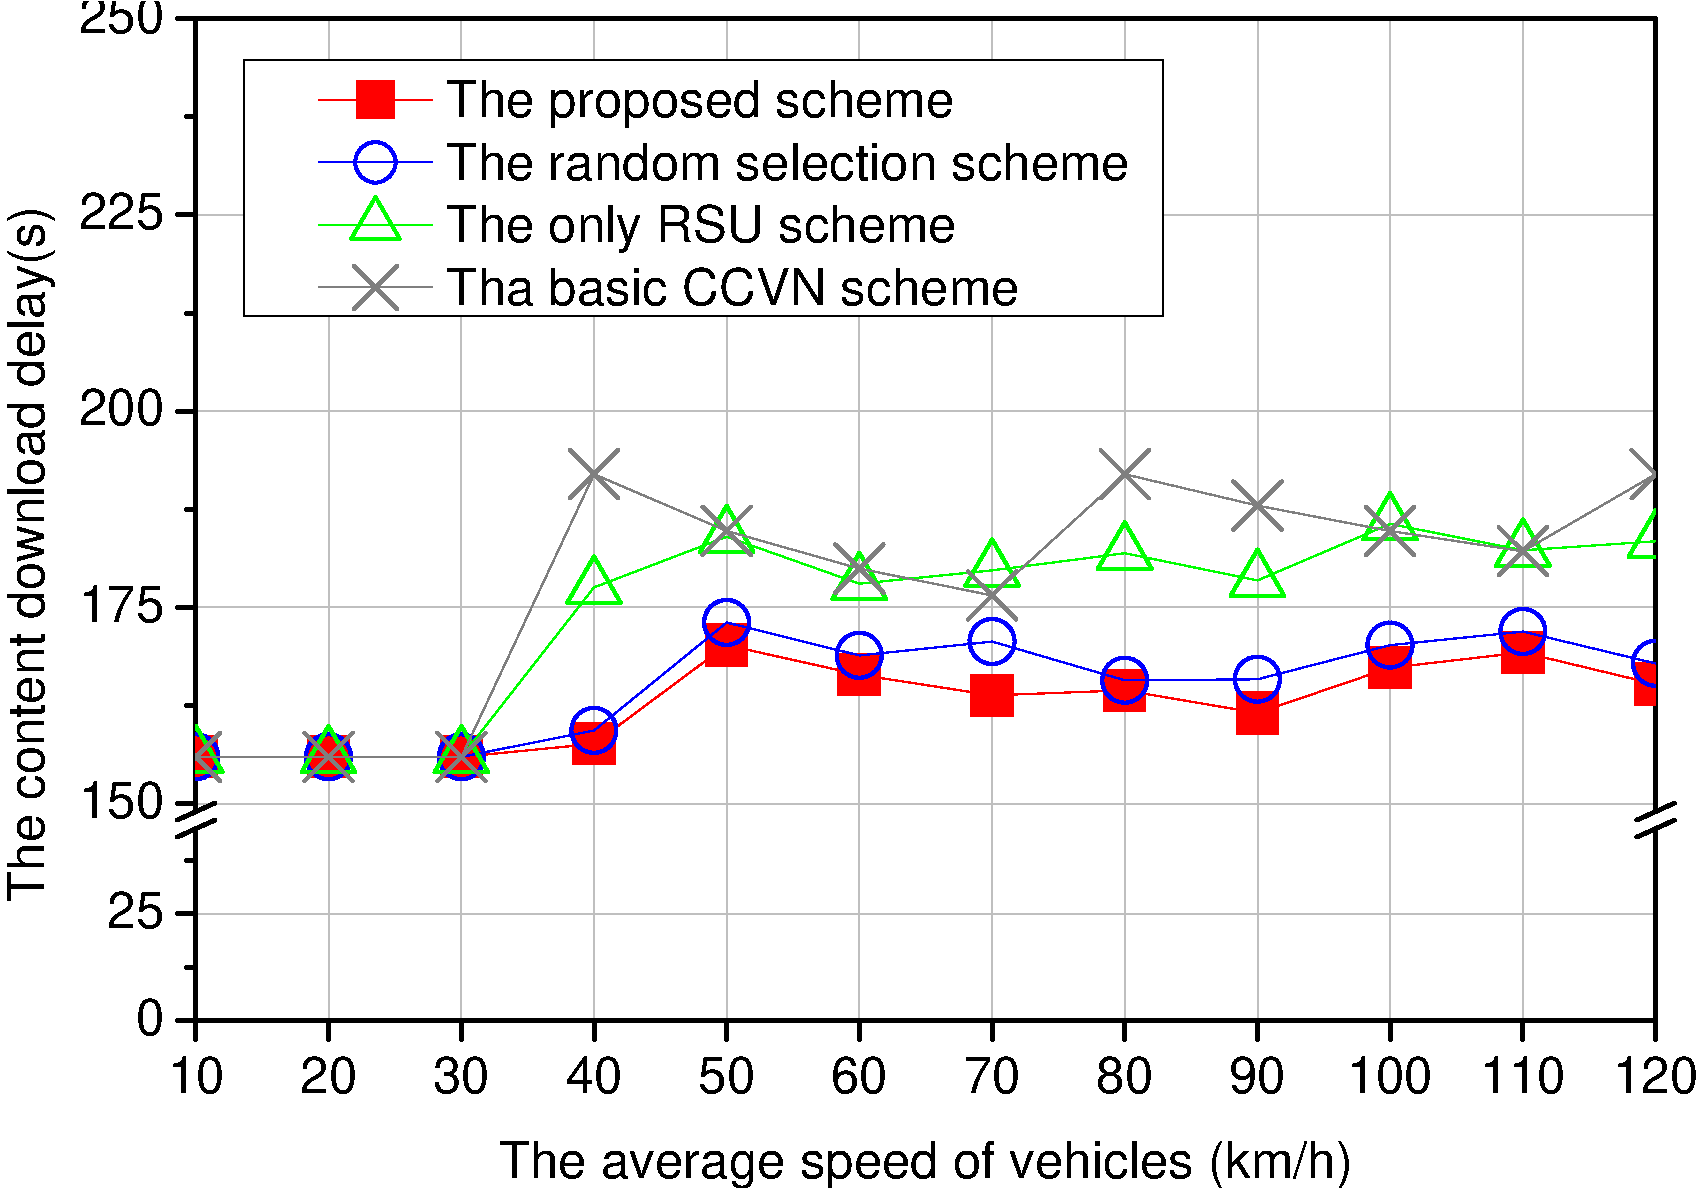
\includegraphics[width=0.48\textwidth]{./graph/S Delay.pdf}}
    \subfigure[]{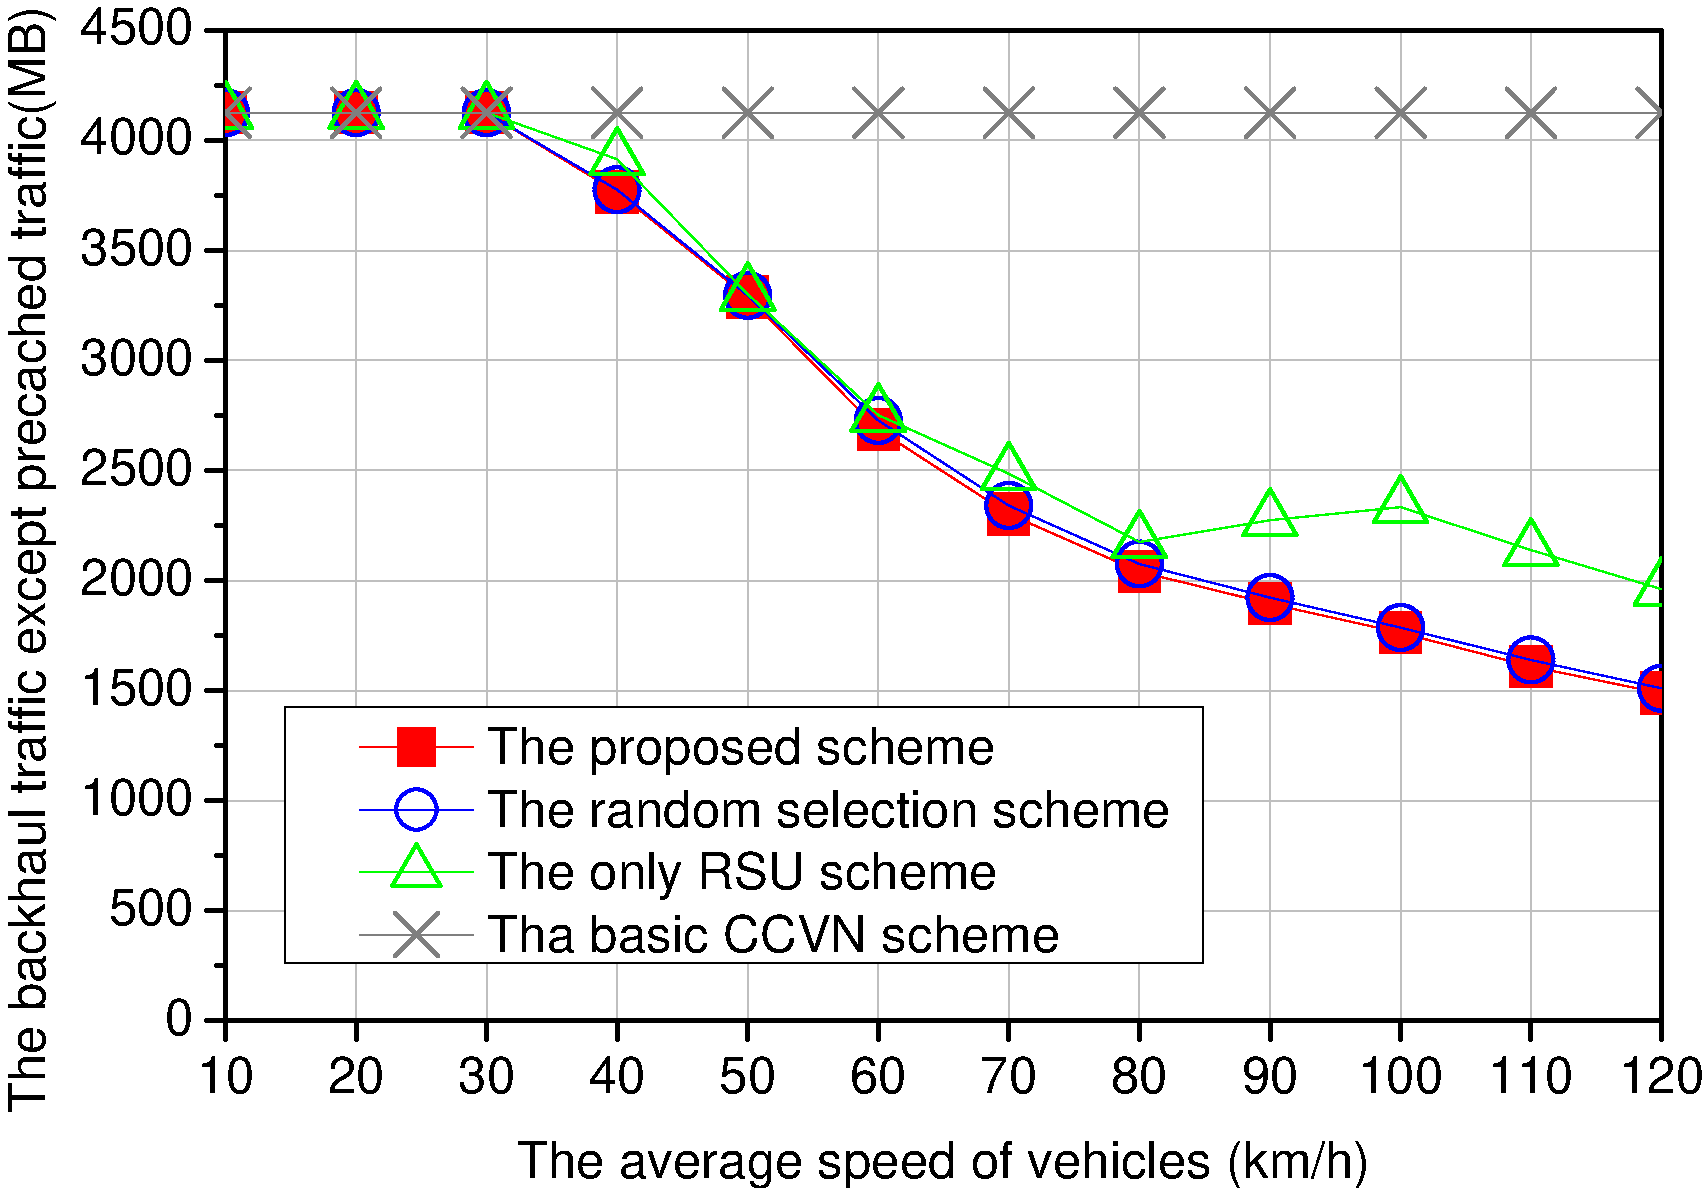
\includegraphics[width=0.48\textwidth]{graph/S Traffic.pdf}}\\
    \subfigure[]{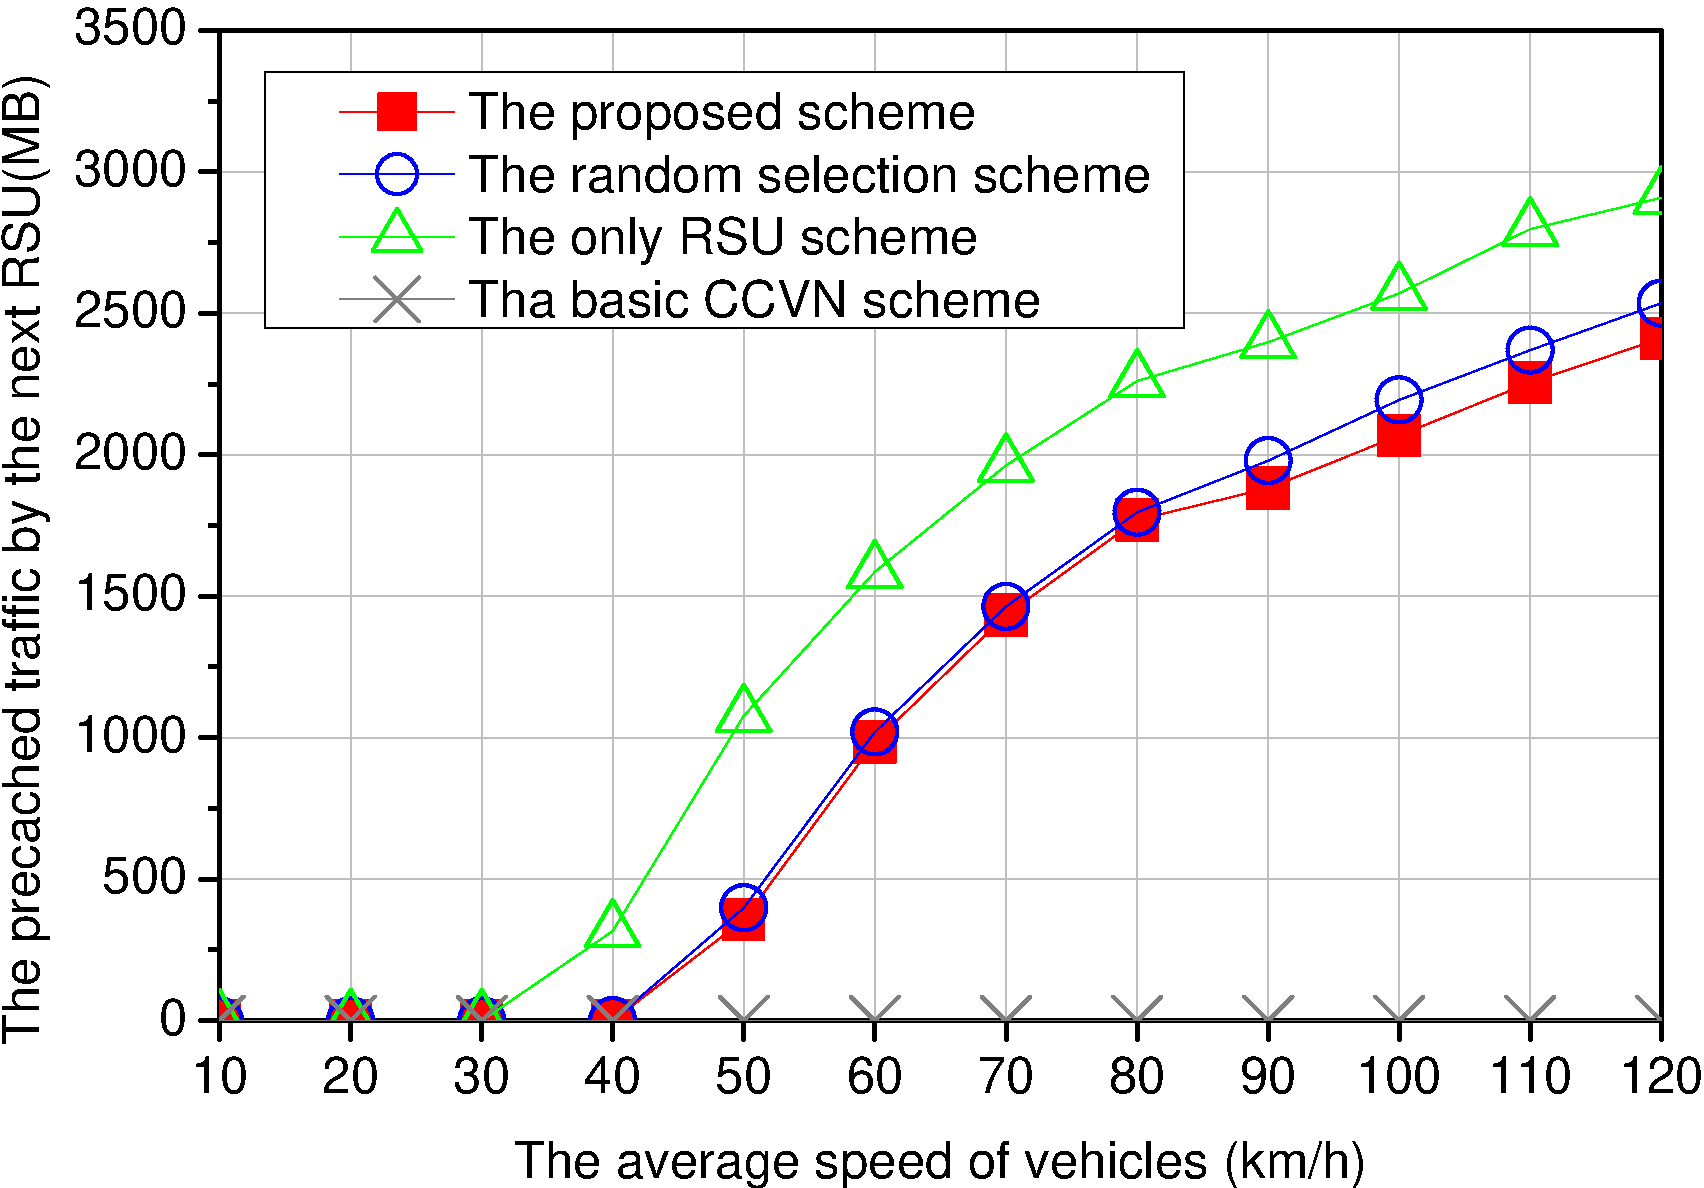
\includegraphics[width=0.48\textwidth]{graph/S Precache.pdf}}
    \subfigure[]{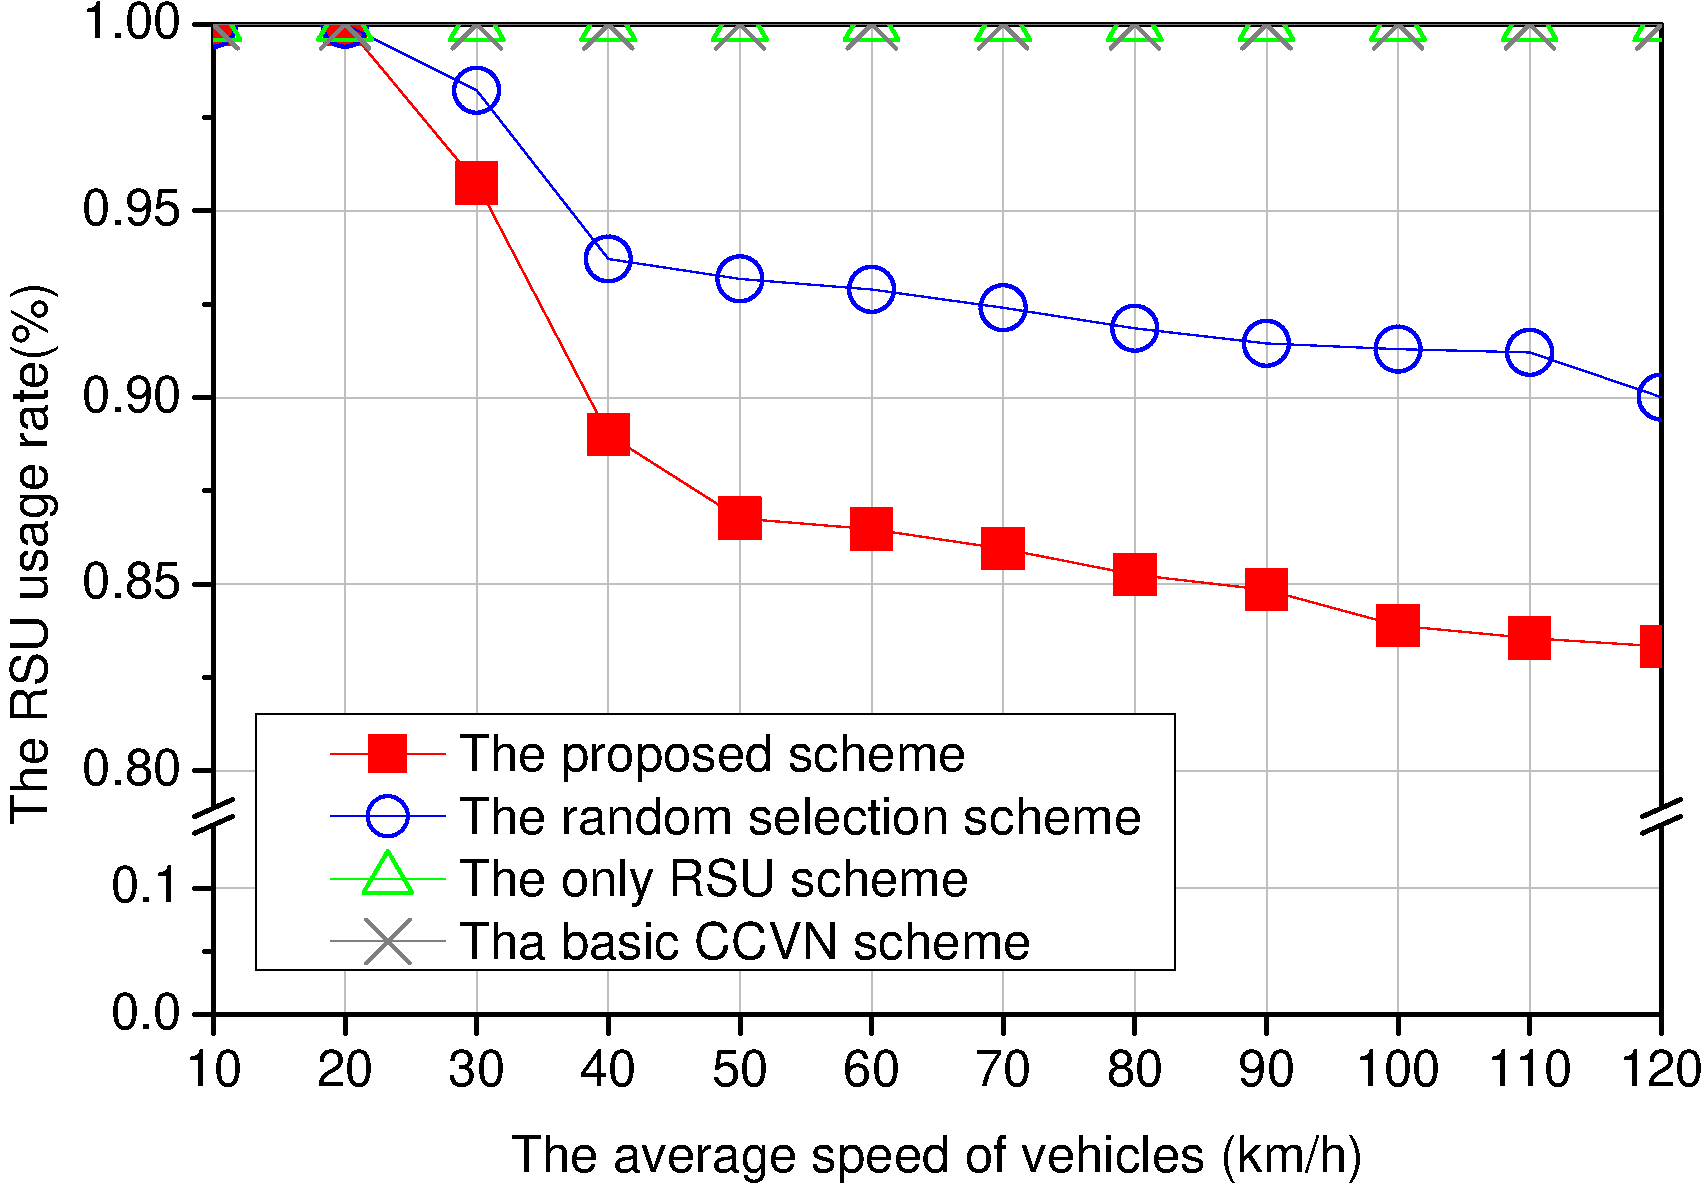
\includegraphics[width=0.48\textwidth]{graph/S RSU use.pdf}}
    \caption{Simulation %MDPI: please check the incomplete ``250'' in subfigure a.
 results for different speeds of the requester vehicle : (\textbf{a}) the content download delay, (\textbf{b}) the backhaul traffic except precached traffic, (\textbf{c}) the precached traffic by next RSU, and (\textbf{d})~the RSU usage rate.}
    \label{fig:d}
\end{figure}




Figure \ref{fig:d}b shows the impact of backhaul traffic, excluding precaching traffic, on the speed of ${V}_{req}$. The backhaul traffic, except for the precaching traffic, is the backhaul traffic consumed by the RSU to relay content from the content server to ${V}_{req}$. Because relaying the content from the content server to ${V}_{req}$ is inefficient in terms of the transmission rate, small backhaul traffic indicates good performance. First, in terms of this indicator, the basic CCVN scheme is unaffected by mobility prediction error because it does not use precaching. In the RSU scheme, only the RSU precaches the content; therefore, it outperforms the basic CCVN scheme. In the case of the random selection scheme, inefficient traffic is consumed less than in the RSU scheme because ${V}_{rel}$ precaches the content. The proposed scheme has the smallest backhaul traffic because ${V}_{rel}$ precaches the maximum available content size in the outage zone.

Figure \ref{fig:d}c shows the relationship between the speed of ${V}_{req}$ and the backhaul traffic consumed by the RSU for precaching. The basic CCVN scheme does not precache the content. Because the proposed scheme uses optimized ${V}_{rel}$, the RSU has the least traffic to precache the content. Compared with the proposed scheme, the random selection scheme performs poorly because it randomly selects ${V}_{rel}$. In the RSU scheme, the next RSU precaches the entire content, except for some of the content that is relayed by the first RSU from the content server to the vehicle. Thus, in this scheme, RSUs consume the most backhaul traffic to precache the content.

Figure \ref{fig:d}d depicts the trends in the involvement of RSUs in providing content according to the speed of the vehicle. ${V}_{req}$ is provided by the RSU in only two schemes that do not use ${V}_{rel}$. Because the proposed scheme uses the optimal ${V}_{rel}$, it uses the least number of RSUs in terms of providing content to ${V}_{req}$. In the case of the random selection scheme, more RSUs are used than in the proposed scheme, because ${V}_{rel}$ is chosen randomly. In these two schemes using ${V}_{rel}$, the performance converges as the connection time with other vehicles, and the dwell time in the outage zone is reduced if ${V}_{req}$ is too fast.

\subsection{Performance for Accuracy of Vehicle Mobility Prediction} \label{sec.5.4}


In Figure \ref{fig:e}, we evaluated the performance according to the size of the guard band applied to compensate for the difference between the predicted and actual mobilities of the vehicle. Figure \ref{fig:e}a presents the content download delay caused by the prediction error when the guard band is applied. The basic CCVN scheme is not affected by prediction errors in vehicle mobility, because it does not use precaching. Only the RSU scheme has an increased size of the content taken from the former RSU or content server owing to prediction error. The two schemes using relaying vehicles take more time to download the entire content, as the size of the content provided by the relaying vehicles decreases if the prediction error of the vehicle mobility is large. However, as the size of the guard band increases, performance degradation from a delay perspective is mitigated.

Figure \ref{fig:e}b depicts the required backhaul traffic, except for precaching, using a guard band to mitigate performance degradation owing to the mobility prediction error. In the basic CCVN scheme, because the RSU does not precache the requested content using the prediction of vehicle mobility, it provides the requested content to the vehicle from the content server via relaying. In the other schemes, if the prediction error increases, backhaul traffic is consumed as much as it differs from the prediction. Because the proposed scheme uses optimized relaying vehicles to provide content to ${V}_{req}$, it consumes the lowest backhaul traffic. However, because accurate prediction is impossible in a real environment, we use a guard band to cover the prediction error. This reduces the amount received using precaching. Therefore, as the size of the additional content to be received increases, so does the size of the guardband prepared to compensate for the error. In addition, if the size of the guard band is increased to cover more prediction errors, the traffic required for preparing the guard band is further increased.

Figure \ref{fig:e}c shows the traffic for precaching owing to the use of the guard band. In all the schemes, if the prediction is perfect, the next RSU precaches the appropriate size content requested by the vehicle. The mobility prediction error is caused by predicting faster or slower than the actual speed of ${V}_{req}$. Because ${V}_{req}$, which is faster than expected, causes a smaller dwell time than the actual dwell time, ${V}_{req}$ is not fully provided with precached content. ${V}_{req}$, which was slower than the actual speed, had a longer dwell time. The RSU precaches a smaller-sized content, consuming less traffic than the actual size of the content that can be received by vehicles with longer dwell times. Thus, if the mobility prediction is incorrect, the traffic consumed by precaching decreases. Because the proposed scheme uses optimized relaying vehicles, the least amount of traffic is consumed to perform the precaching. It consumes more traffic to prepare the guard band by applying it to cope with prediction errors.

Figure \ref{fig:e}d presents the RSU usage ratio with the adjustment of the guard band. The two schemes that did not use relaying vehicles provided content to ${V}_{req}$ using only the RSU. The proposed scheme uses less RSU than the random selection scheme, which randomly selects relaying vehicles. With a large mobility prediction error, the guardband can cover the error to reduce the RSU usage ratio by utilizing the guardband contained in the relaying vehicles. If the mobility prediction error exceeds the size covered by the guard band, the performance improvement converges.

In Figure \ref{fig:my_label}, we evaluate the hit ratio for the precached content by adding a guard band. The basic CCVN scheme does not use precaching. If the mobility prediction error is small, the hit ratio is more affected by the connection time between ${V}_{req}$ and ${V}_{rel}$ than by the dwell time on the RSU. Therefore, the hit ratio in the RSU scheme was higher than that in random selection in that case. Otherwise, if the mobility prediction error is large, the hit rate in the RSU scheme decreases dramatically because of the large impact of the dwell time on the RSU. The proposed scheme had the highest hit ratio because of the selection of optimized relaying vehicles. Furthermore, the large size of the guard band alleviates the reduced hit ratio owing to the mobility prediction error. This indicates that most of the traffic consumed was directed to ${V}_{req}$.

\begin{figure}[H]
    \subfigure[]{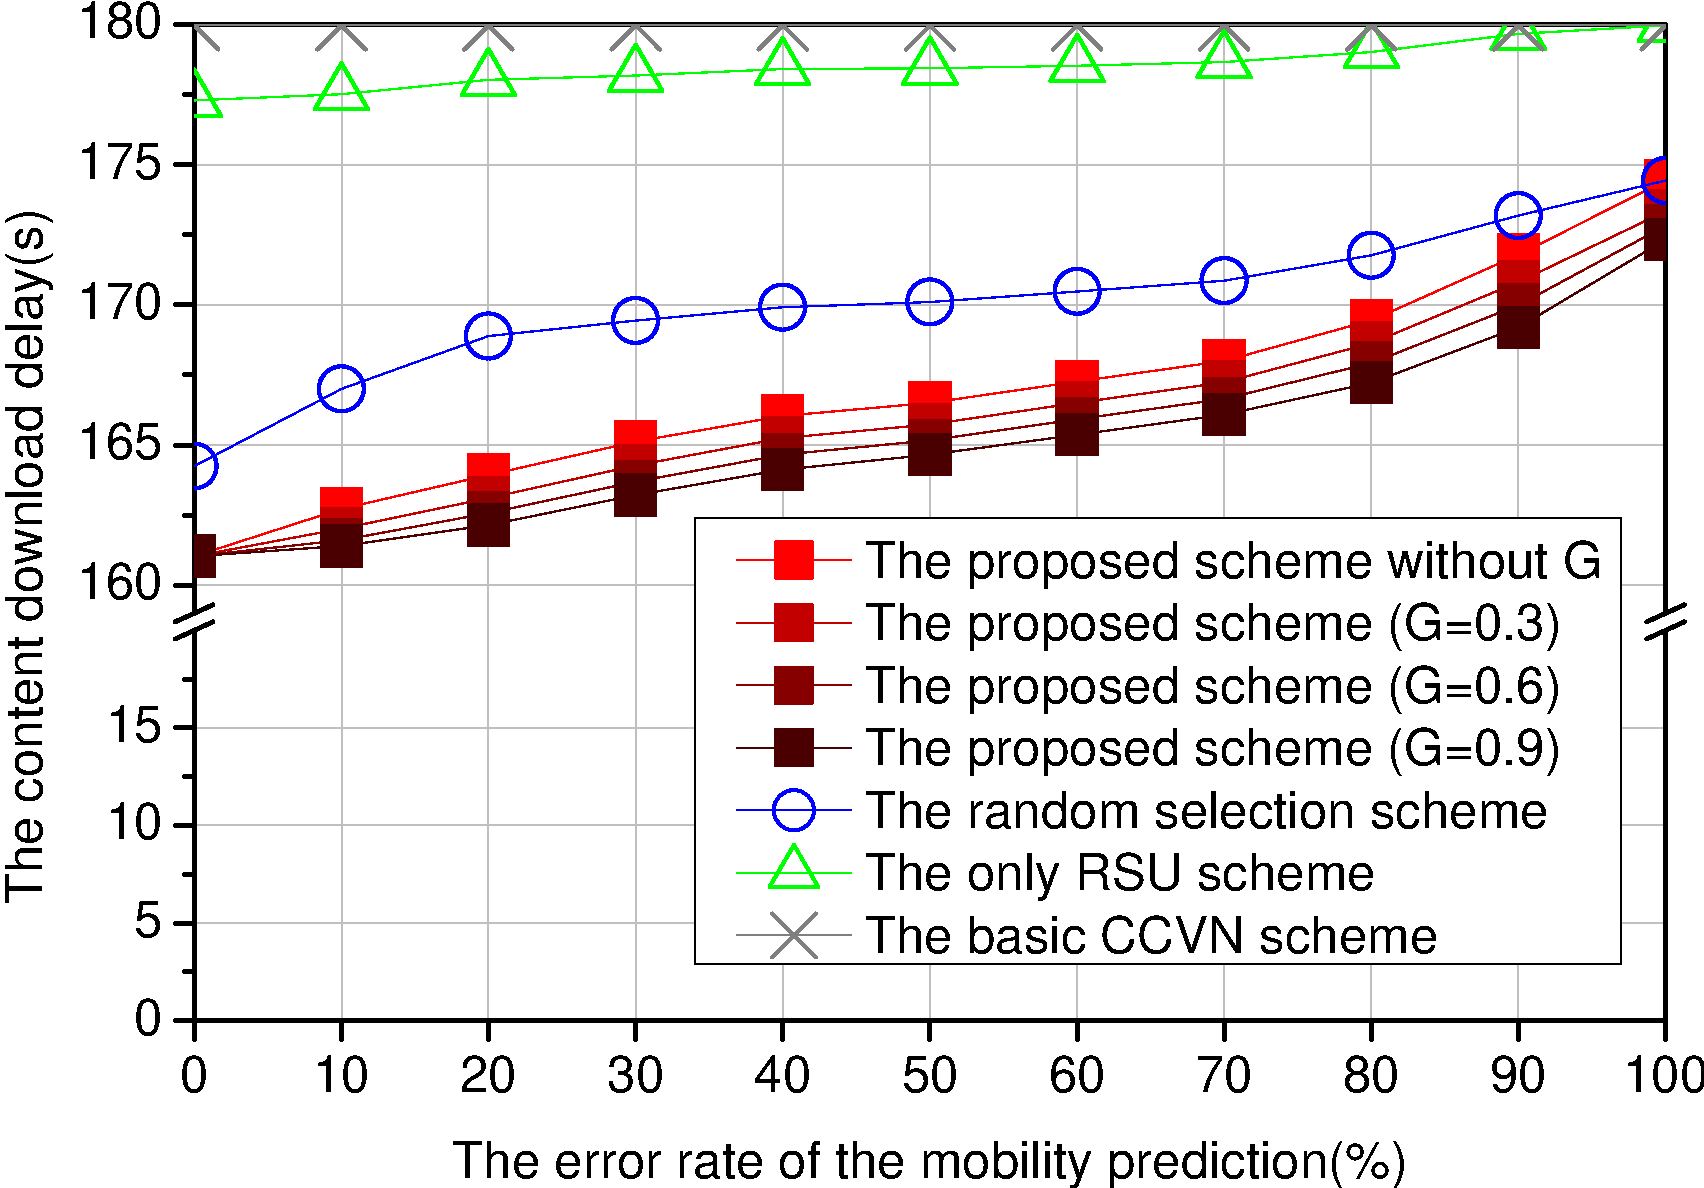
\includegraphics[width=0.48\textwidth]{./graph/G Delay.pdf}}
    \subfigure[]{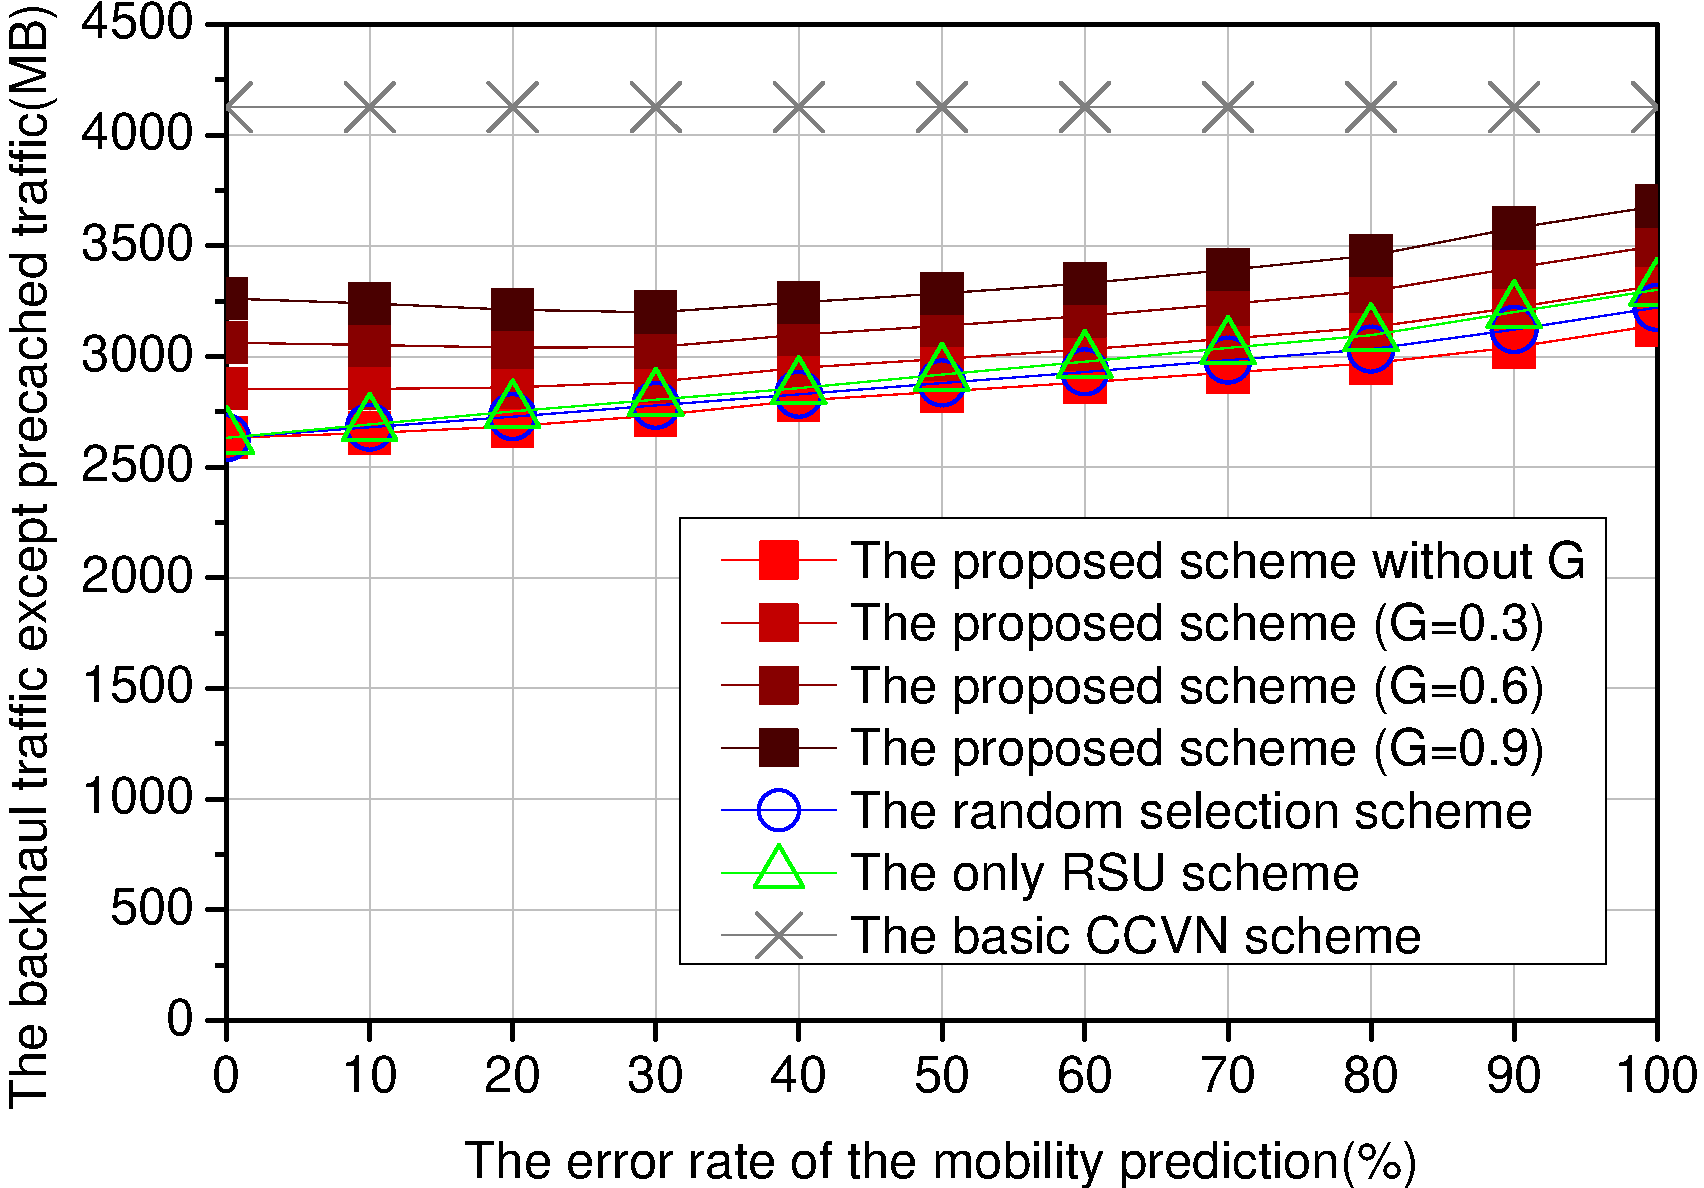
\includegraphics[width=0.48\textwidth]{graph/G Traffic.pdf}}\\
    \subfigure[]{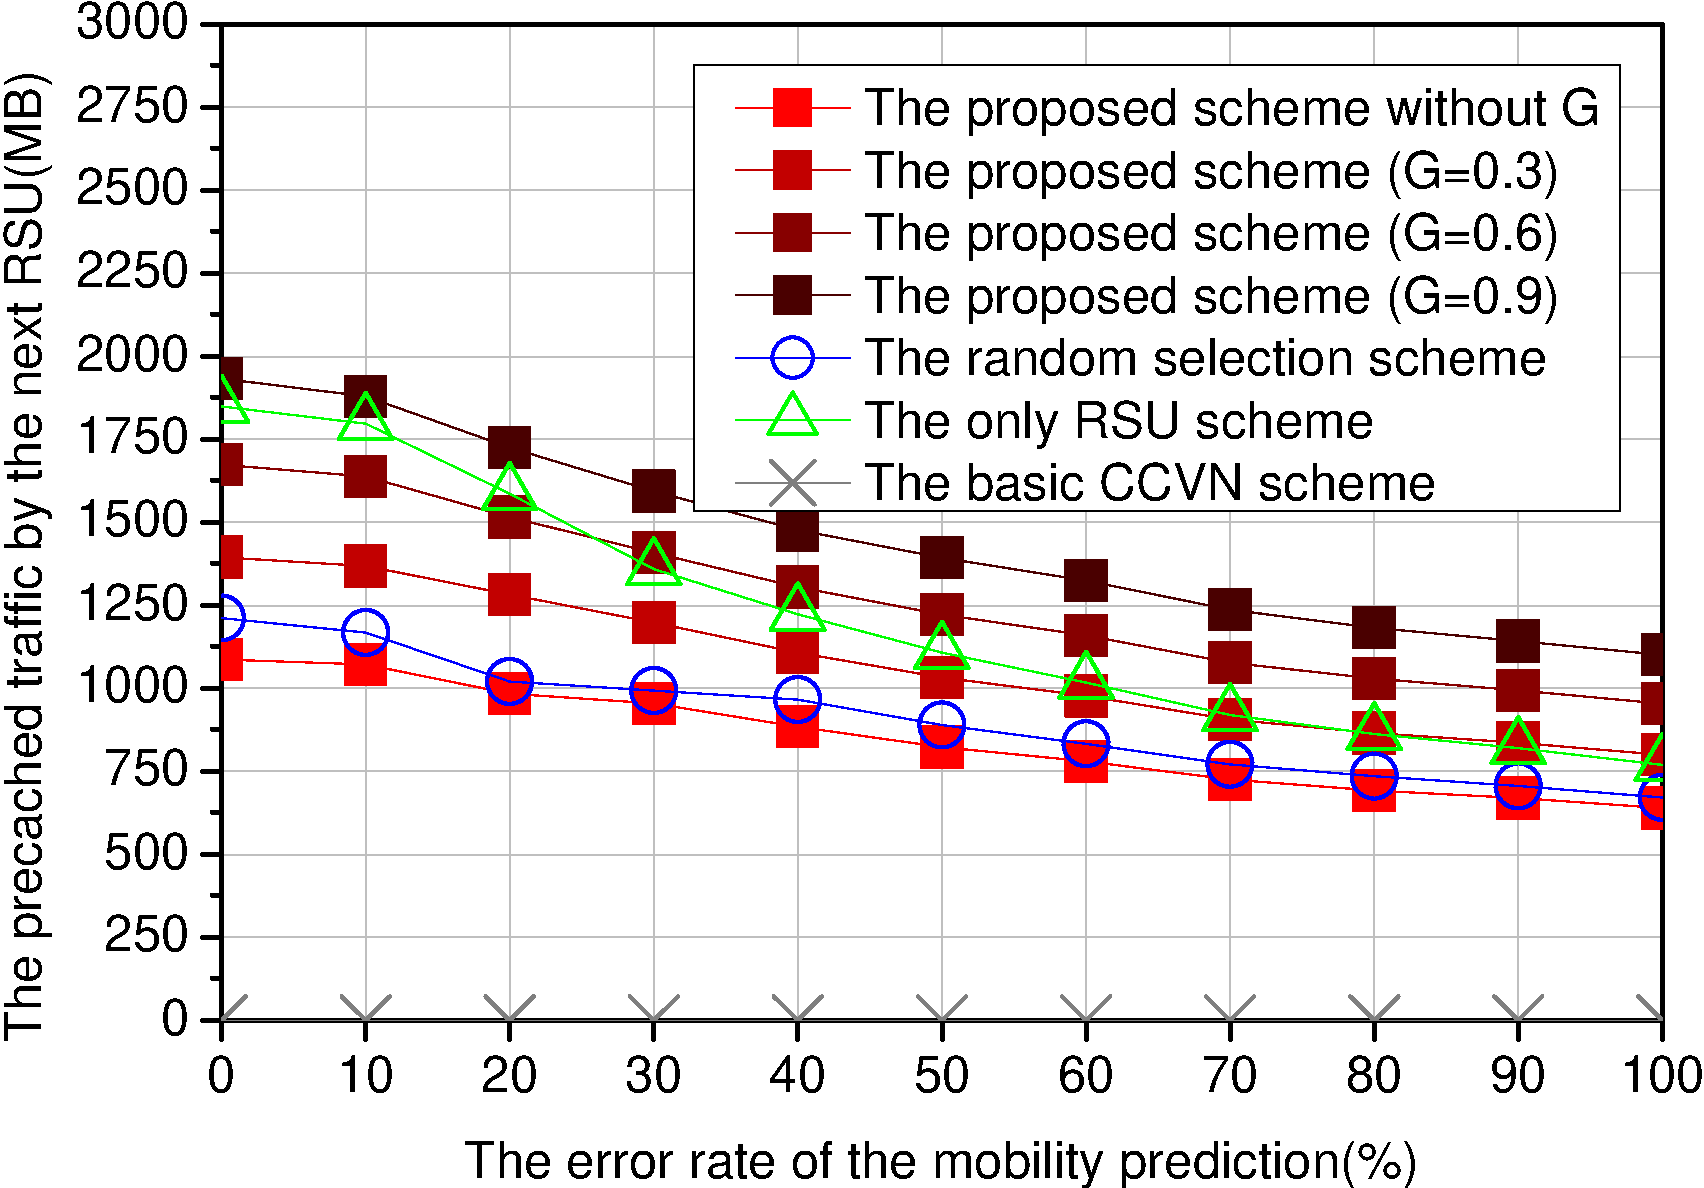
\includegraphics[width=0.48\textwidth]{graph/G Precache.pdf}}
    \subfigure[]{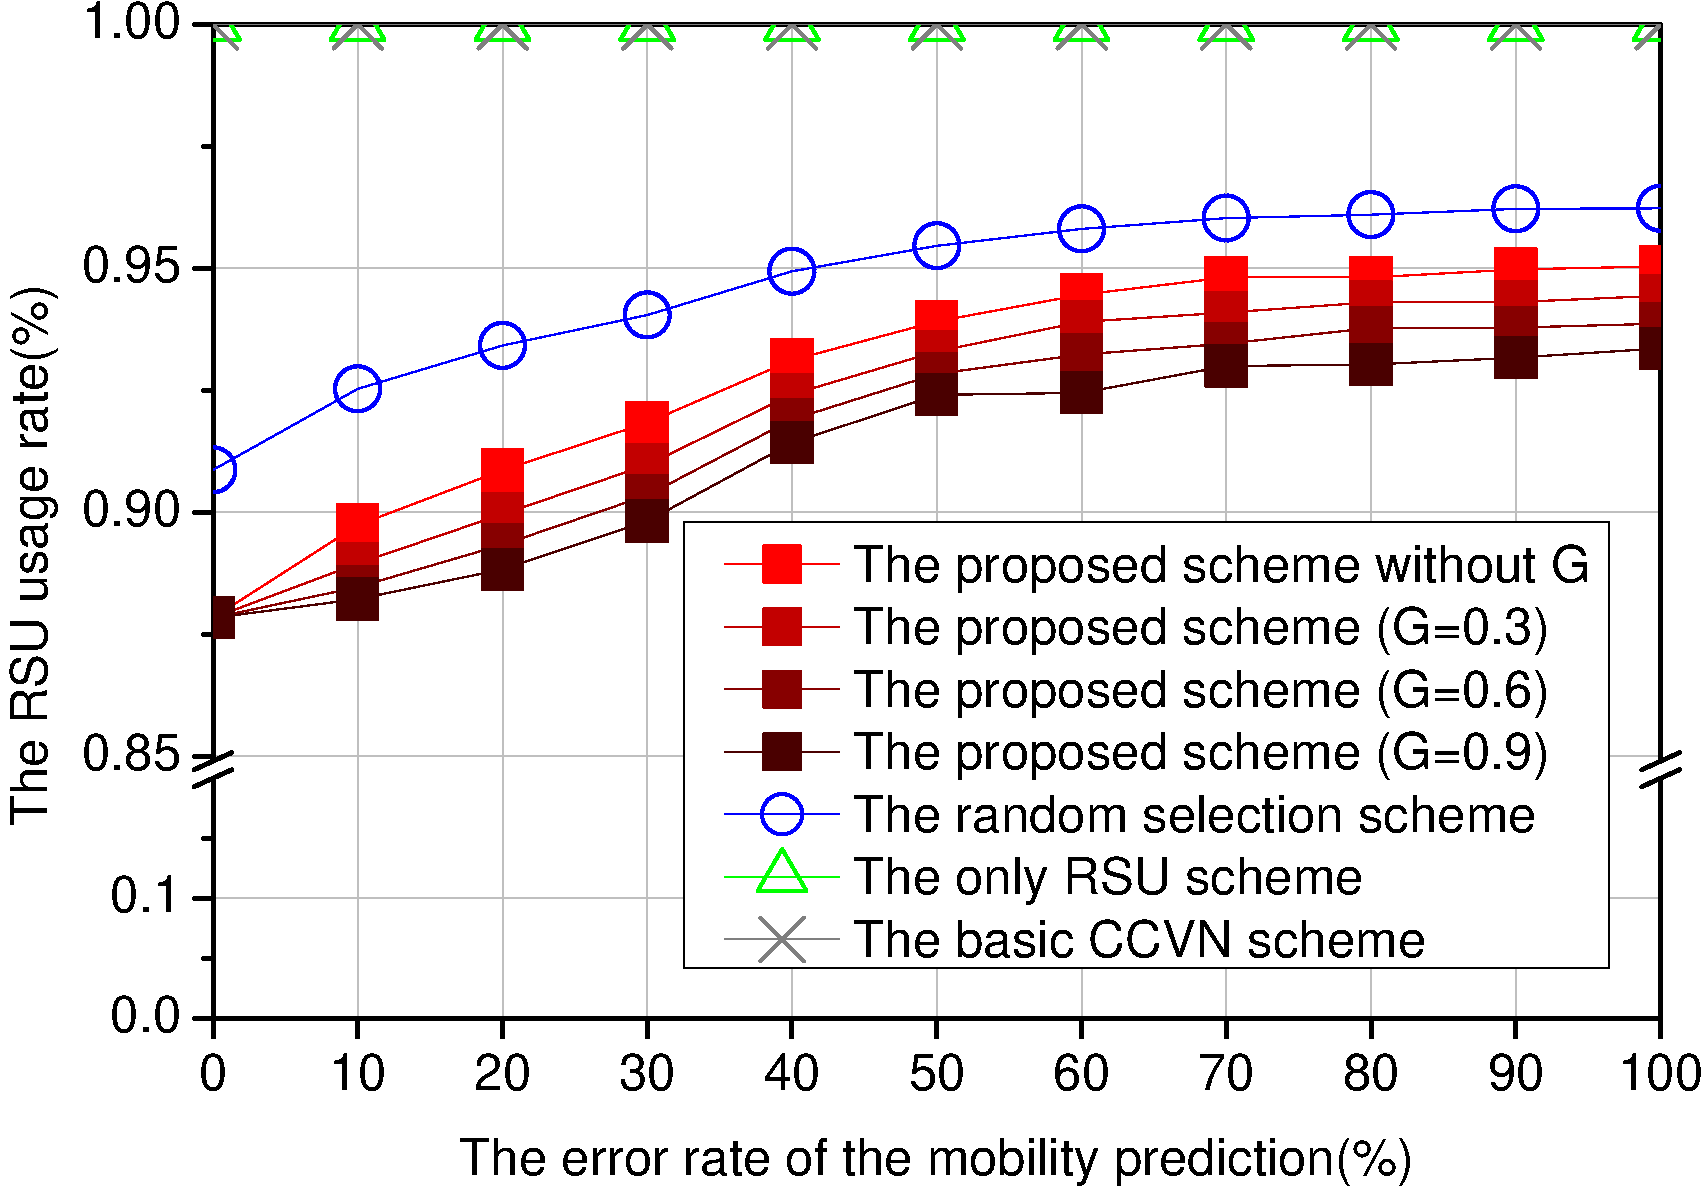
\includegraphics[width=0.48\textwidth]{graph/G RSU use.pdf}}
    \caption{Simulation results for different error rates of the mobility predictions with various guardbands: (\textbf{a}) the content download delay, (\textbf{b}) the backhaul traffic except precached traffic, (\textbf{c}) the precached traffic by next RSU and (\textbf{d}) the RSU usage rate.}
    \label{fig:e}
\end{figure}



\begin{figure}[H]
    %\centering
    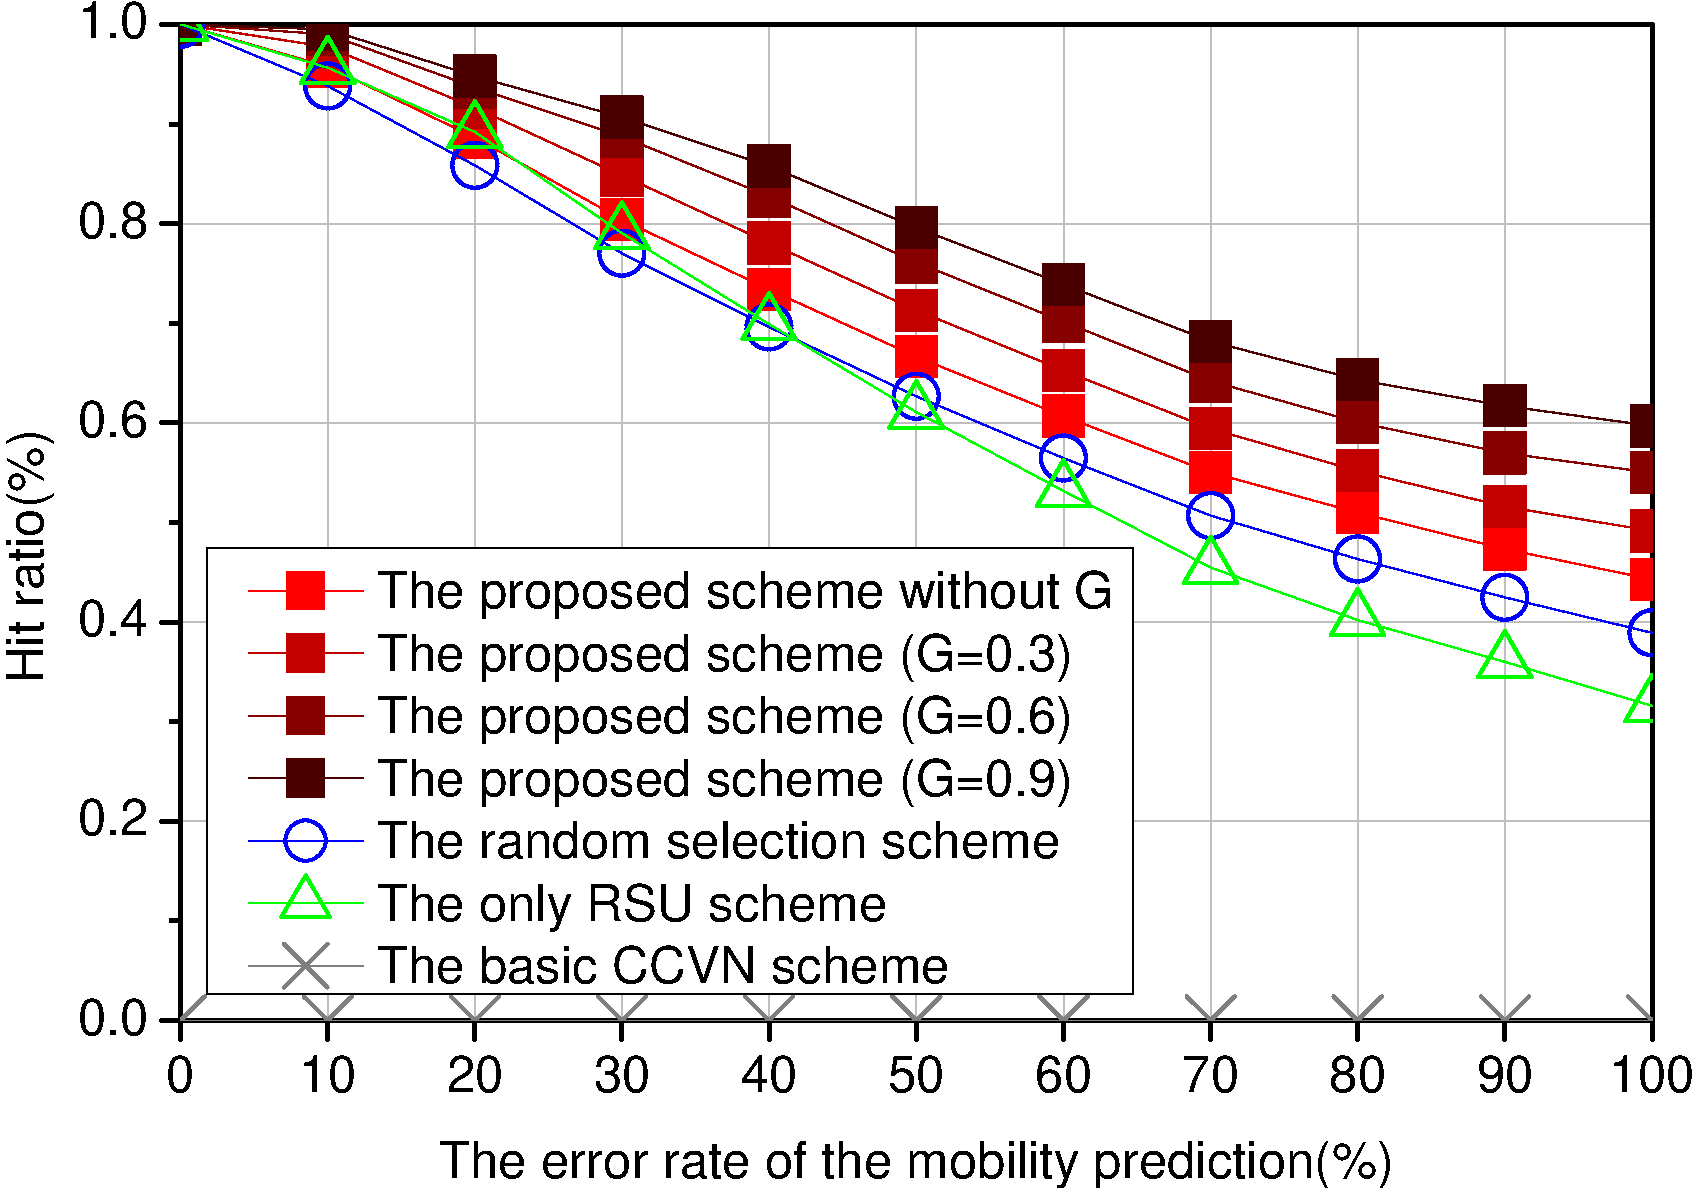
\includegraphics[width=10 cm]{graph/G Hit ratio.pdf}
    \caption{The hit ratio for the error rate of the mobility prediction. }
    \label{fig:my_label}
\end{figure}
\newpage
\section{Discussion} \label{sec.dis}
In this section, we discuss several issues related to the cooperative content precaching scheme and its viability in a practical context.

\subsection{Security of Privacy}
In the proposed scheme, the trajectory and mobility information of vehicles are shared with RSUs and other vehicles to achieve better precaching performance. In addition, the content that a vehicle wishes to download is cached or precached distributively to the RSUs or other vehicles. In this case, the requester vehicle’s private information, which includes the mobility and preference for the content, is disclosed to others. Because disclosed information about the requester vehicle can be used to attack or threaten the user, it must be protected. Therefore, many studies have proposed protection schemes to hide private information, while the precaching service is served to the requester vehicle using blockchain or other technologies~\cite{Yellanki2020Secu, Chai2019AHie}. Reliable precaching services can only be used when safety is guaranteed. Thus, when the proposed scheme uses the proper security protocol for precaching, it can achieve reliable service while maintaining high network performance.

\subsection{Energy Consumption}
In vehicular networks, saving energy is one of the most important issues to achieve a longer driving time owing to the limitation of the battery. In the proposed scheme, almost all the computing processes to precache the content are conducted at RSUs. However, the relaying vehicle spends the energy required to reach the requested content and provide it to the requester vehicle. Therefore, several studies have been conducted to reduce the energy consumed in precaching the requested content~\cite{Tran2017Mobe, Shen2020ABlo, Ahani2018OnOp, Dong2020APro}.
To save energy, it is possible to increase the delay in content download and backhaul traffic used to serve the precaching service~\cite{Shen2020ABlo}.
Thus, this is a very sensitive issue for reducing the consumed energy to precache the content at RSUs or other vehicles. When a proper energy-saving method is considered in the proposed scheme, the scheme can be improved in terms of energy and other network performances.

\subsection{Combination with 5G Technology}
For viability in the practical context of a precaching scheme, it is necessary to consider 5G or 6G technologies. To provide precaching service to vehicles in 5G, numerous studies have been conducted~\cite{Mehteroglu2017Sema, Liang2018Enab}. Because many parameters and environments have become standards for 5G, these must be considered when conducting a precaching service in a real scenario. In 5G technology, many modules are provided for each purpose. These modules can be considered to improve the network performance, such as delay, traffic, or security problems in the proposed scheme.

\section{Conclusions} \label{sec6}
In this study, we propose a cooperative content precaching scheme based on the mobility information of vehicles to enhance the performance of content downloads in ICVNs. In contrast to the existing schemes, our scheme cooperatively used both vehicles and RSUs for the precaching content. For content precaching based on the mobility information of vehicles, our scheme selected both the optimal vehicle for relaying content in the outage zone and the next RSU to download the content in the coverage of the RSU. Our scheme calculated the optimal content precaching amount for each optimal relaying vehicle and the next downloading RSU using a mathematical model that used both the dwell time of vehicles in an RSU and contact time between vehicles. To compensate for the error of the vehicle mobility prediction to determine both the dwell and contact times, our scheme added a guard band to the optimal content precaching amount. For mobility prediction errors, the guard band is calculated with the error rate of both the dwell and contact times, and it is adjusted in the trade-off between the expected reduced delay and backhaul traffic. We conducted simulations to compare the performance of our scheme with the performances of existing schemes from three perspectives: Various environmental factors, characteristics related to requester vehicles, and accuracy of vehicle mobility prediction. Simulation results verify that our scheme achieves better performance than existing schemes in terms of the content download delay, backbone traffic, precaching traffic, RSU usage ratio, and hit ratio. In future work, we will consider other vehicles or drones that have already cached the requested content, as providers without using additional backhaul traffic. In addition, using an additional server, we can employ a machine learning method to improve the performance of the proposed scheme.



%\section{Patents}
%This section is not mandatory, but may be added if there are patents resulting from the work reported in this manuscript.
%%%%%%%%%%%%%%%%%%%%%%%%%%%%%%%%%%%%%%%%%%
\vspace{6pt}
%%%%%%%%%%%%%%%%%%%%%%%%%%%%%%%%%%%%%%%%%%
%% optional
%\supplementary{The following supporting information can be downloaded at:  \linksupplementary{s1}, Figure S1: title; Table S1: title; Video S1: title.}

% Only for the journal Methods and Protocols:
% If you wish to submit a video article, please do so with any other supplementary material.
% \supplementary{The following supporting information can be downloaded at: \linksupplementary{s1}, Figure S1: title; Table S1: title; Video S1: title. A supporting video article is available at doi: link.}
%%%%%%%%%%%%%%%%%%%%%%%%%%%%%%%%%%%%%%%%%%
\authorcontributions{Conceptualization, J.B.; methodology, Y.N.; software, Y.N.; validation, H.C., Y.S., J.B.%, D.M.
; writing---original draft preparation, Y.N.; writing---review and editing, H.C., E.L.; supervision, E.L.; %funding acquisition, E.L.
All authors have read and agreed to the published version of the~manuscript.}

\funding{This work was supported by the National Research Foundation of Korea(NRF) grant funded by the Korea government(Ministry of Science and ICT) (No. NRF\-2022R1A2C1010121).
This study was conducted with the support of the Korea Institute of Industrial Technology (P0008421) funded by the government (Ministry of Trade, Industry and Energy).
}
\institutionalreview{Not applicable.}
\informedconsent{Not applicable.}
\dataavailability{Not applicable.}
\conflictsofinterest{The authors declare no conflict of~interest.}
%%%%%%%%%%%%%%%%%%%%%%%%%%%%%%%%%%%%%%%%%%
%% Only for journal Encyclopedia
%\entrylink{The Link to this entry published on the encyclopedia platform.}
%%%%%%%%%%%%%%%%%%%%%%%%%%%%%%%%%%%%%%%%%%
%% Optional
\appendixtitles{no} % Leave argument "no" if all appendix headings stay EMPTY (then no dot is printed after "Appendix A"). If the appendix sections contain a heading then change the argument to "yes".

%\section[\appendixname~\thesection]{}
%All appendix sections must be cited in the main text. In the appendices, Figures, Tables, etc. should be labeled, starting with ``A''---e.g., Figure A1, Figure A2, etc.
%%%%%%%%%%%%%%%%%%%%%%%%%%%%%%%%%%%%%%%%%%
\begin{adjustwidth}{-\extralength}{0cm}
\reftitle{References} \begin{thebibliography}{999}
\bibitem{Karagiannis2011Vehicular} %1
Karagiannis, G.; Altintas, O.; Ekici, E.; Heijenk, G.; Jarupan, B.; Lin, K.; Weil, T. Vehicular Networking: A Survey and Tutorial on Requirements, Architectures, Challenges, Standards and Solutions. \emph{IEEE Commun. Surv. Tutorials} \textbf{2011}, \emph{13}, 584--616. https://doi.org/10.1109/surv.2011.061411.00019.

\bibitem{Awang2017} %2
Awang, A.; Husain, K.; Kamel, N.; Aissa, S. Routing in Vehicular Ad-hoc Networks: A Survey on Single- and Cross-Layer Design Techniques, and Perspectives. \emph{IEEE Access} \textbf{2017}, \emph{5}, 9497–9517. https://doi.org/10.1109/access.2017.2692240.

\bibitem{Shahwani2021} %3
Shahwani, H.; Shah, S.A.; Ashraf, M.; Akram, M.; Jeong, J.; Shin, J. A comprehensive survey on data dissemination in Vehicular Ad Hoc Networks. \emph{Veh. Commun. }\textbf{2021}, \emph{34}, 100420. https://doi.org/10.1016/j.vehcom.2021.100420.

\bibitem{An2016Sec}%4
An, K.; Lin, M.; Ouyang, J.; Zhu, W.-P. Secure Transmission in Cognitive Satellite Terrestrial Networks. \emph{IEEE J. Sel. Areas Commun. }\textbf{2016}, \emph{34}, 3025–3037. https://doi.org/10.1109/jsac.2016.2615261.

\bibitem{Lin2022Ref} %5
Lin, Z.; Niu, H.; An, K.; Wang, Y.; Zheng, G.; Chatzinotas, S.; Hu, Y. Refracting RIS-Aided Hybrid Satellite-Terrestrial Relay Networks: Joint Beamforming Design and Optimization. \emph{IEEE Trans. Aerosp. Electron. Syst.} \textbf{2022}, \emph{58}, 3717--3724. https://doi.org/10.1109/taes.2022.3155711

\bibitem{Lin2021Sup} %6
Lin, Z.; Lin, M.; de Cola, T.; Wang, J.-B.; Zhu, W.-P.; Cheng, J. Supporting IoT With Rate-Splitting Multiple Access in Satellite and Aerial-Integrated Networks. \emph{IEEE Internet Things J. }\textbf{2021}, \emph{8}, 11123--11134. https://doi.org/10.1109/jiot.2021.3051603

\bibitem{Lin2022SLN} %7
Lin, Z.; An, K.; Niu, H.; Hu, Y.; Chatzinotas, S.; Zheng, G.; Wang, J. SLNR-based Secure Energy Efficient Beamforming in Multibeam Satellite Systems. \emph{IEEE Trans. Aerosp. Electron. Syst. }\textbf{2022}, 1--4, \emph{early access}. https://doi.org/10.1109/taes.2022.3190238.

\bibitem{Euisin2014} %8
Lee, E.; Lee, E.-K.; Gerla, M.; Oh, S.Y. Vehicular cloud networking: Architecture and design principles. \emph{IEEE Commun. Mag.} \textbf{2014}, \emph{52}, 148–155. https://doi.org/10.1109/mcom.2014.6736756.

\bibitem{Zhang2018} %9
Zhang, S.; Chen, J.; Lyu, F.; Cheng, N.; Shi, W.; Shen, X. Vehicular Communication Networks in the Automated Driving Era. \emph{IEEE Commun. Mag.} \textbf{2018}, \emph{56}, 26–32. https://doi.org/10.1109/mcom.2018.1701171.

\bibitem{Khelifi2020} %10
\textls[-15]{Khelifi, H.; Luo, S.; Nour, B.; Moungla, H.; Faheem, Y.; Hussain, R.; Ksentini, A. Named Data Networking in Vehicular Ad Hoc Networks: State-of-the-Art and Challenges. \emph{IEEE Commun. Surv. Tutorials }\textbf{2019}, \emph{22}, 320–351. https://doi.org/10.1109/comst.2019.2894816.}

\bibitem{Cheng2015} %11
Cheng, X.; Yang, L.; Shen, X. D2D for Intelligent Transportation Systems: A Feasibility Study. \emph{IEEE Trans. Intell. Transp. Syst.} \textbf{2015}, \emph{16}, 1784–1793. https://doi.org/10.1109/tits.2014.2377074.

\bibitem{Wang2016} %12
Wang, Y.; Zheng, J.; Mitton, N. Delivery Delay Analysis for Roadside Unit Deployment in Vehicular Ad Hoc Networks With Intermittent Connectivity. \emph{IEEE Trans. Veh. Technol. }\textbf{2015}, \emph{65}, 8591–8602. https://doi.org/10.1109/tvt.2015.2506599.

\bibitem{Lopes2019} %13
%L. H. S. Lopes, R. A. F. Mini and F. Cunha, ``A V2X Approach for Data Dissemination in Vehicular Ad Hoc Networks,'' \textit{2019 IEEE Symposium on Computers and Communications (ISCC)}, 2019, pp. 1-6, doi: 10.1109/ISCC47284.2019.8969698.
Lopes, L.H.S.; Mini, R.A.F.; Cunha, F. A V2X Approach for Data Dissemination in Vehicular Ad Hoc Networks.  In Proceedings of the 2019 IEEE Symposium on Computers and Communications (ISCC), \hl{Barcelona, Spain, 29~June--3~July~2019; }%MDPI: We added the location and date of the conference. Please confirm.
 pp. 1--6. https://doi.org/10.1109/iscc47284.2019.8969698.

\bibitem{Wang2019} %14
Wang, X.; Li, Y. Content Delivery Based on Vehicular Cloud. \emph{IEEE Trans. Veh. Technol.} \textbf{2019}, \emph{69}, 2105–2113. https://doi.org/10.1109/\linebreak tvt.2019.2959799.

\bibitem{Ko2021} %15
Ko, B.; Liu, K.; Son, S.H.; Park, K.-J. RSU-Assisted Adaptive Scheduling for Vehicle-to-Vehicle Data Sharing in Bidirectional Road Scenarios. \emph{IEEE Trans. Intell. Transp. Syst.} \textbf{2020}, \emph{22}, 977–989. https://doi.org/10.1109/tits.2019.2961705.

\bibitem{Haung2021} %16
Huang, W.; Li, P.; Li, B.; Zhang, T. DMP: Content Delivery with Dynamic Movement Pattern in Vehicular Networks. \emph{IEEE Trans. Big Data} \textbf{2021}, \emph{8}, 1. https://doi.org/10.1109/tbdata.2021.3050777.

\bibitem{Reis2014Deploying} %17
Reis, A.B.; Sargento, S.; Neves, F.; Tonguz, O.K. Deploying Roadside Units in Sparse Vehicular Networks: What Really Works and What Does Not. \emph{IEEE Trans. Veh. Technol.} \textbf{2013}, \emph{63}, 2794–2806. https://doi.org/10.1109/tvt.2013.2292519.

\bibitem{Kim2017} %18
Kim, D.; Velasco, Y.; Wang, W.; Uma, R.N.; Hussain, R.; Lee, S. A New Comprehensive RSU Installation Strategy for Cost-Efficient VANET Deployment. \emph{IEEE Trans. Veh. Technol.} \textbf{2016}, \emph{66}, 4200--4211. https://doi.org/10.1109/tvt.2016.2598253.

\bibitem{Su2017NextGeneration} %19
Su, Z.; Hui, Y.; Yang, Q. The Next Generation Vehicular Networks: A Content-Centric Framework. \emph{IEEE Wirel. Commun.} \textbf{2017}, \emph{24}, 60–66. https://doi.org/10.1109/mwc.2017.1600195wc.

\bibitem{Rao2013Proactive} %20
%Y. Rao, H. Zhou, D. Gao, H. Luo and Y. Liu, ``Proactive Caching for Enhancing User-Side Mobility Support in Named Data Networking,'' \textit{2013 Seventh International Conference on Innovative Mobile and Internet Services in Ubiquitous Computing}, 2013, pp. 37-42, doi: 10.1109/IMIS.2013.16.
Rao, Y.; Zhou, H.; Gao, D.; Luo, H.; Liu, Y. Proactive Caching for Enhancing User-Side Mobility Support in Named Data Networking. In Proceedings of the 2013 Seventh International Conference on Innovative Mobile and Internet Services in Ubiquitous Computing, \hl{Taichung, Taiwan, 3--5 July 2013}; pp.~37–42. https://doi.org/10.1109/imis.2013.16.

\bibitem{Wang2017} %21
%Y. Wang, Y. Liu, J. Zhang, H. Ye and Z. Tan, ``Cooperative Store–Carry–Forward Scheme for Intermittently Connected Vehicular Networks,'' in \textit{IEEE Transactions on Vehicular Technology}, vol. 66, no. 1, pp. 777-784, Jan. 2017, doi: 10.1109/TVT.2016.2536059.
Wang, Y.; Liu, Y.; Zhang, J.; Ye, H.; Tan, Z. Cooperative Store-Carry-Forward Scheme for Intermittently Connected Vehicular Networks. \emph{IEEE Trans. Veh. Technol.} \textbf{2017}, \emph{66}, 777--784. https://doi.org/10.1109/tvt.2016.2536059.

\bibitem{Suthaputchakun2018} %22
Suthaputchakun, C.; Sun, Z. Multihop Broadcast Protocol in Intermittently Connected Vehicular Networks. \emph{IEEE Trans. Aerosp. Electron. Syst.} \textbf{2017}, \emph{54}, 616–628. https://doi.org/10.1109/taes.2017.2761140.

\bibitem{Wu2013Adaptive} %23
Wu, D.; Zhu, G.; Zhao, D. Adaptive Carry-Store Forward Scheme in Two-Hop Vehicular Delay Tolerant Networks. \emph{IEEE Commun. Lett.} \textbf{2013}, \emph{17}, 721–724. https://doi.org/10.1109/lcomm.2013.022713.130123.

\bibitem{Zhou2019} %24
Zhou, H.; Cheng, N.; Wang, J.; Chen, J.; Yu, Q.; Shen, X. Toward Dynamic Link Utilization for Efficient Vehicular Edge Content Distribution. \emph{IEEE Trans. Veh. Technol.} \textbf{2019}, \emph{68}, 8301–8313. https://doi.org/10.1109/tvt.2019.2921444.

\bibitem{Wang2016Mobility} %25
Wang, R.; Peng, X.; Zhang, J.; Letaief, K.B. Mobility-aware caching for content-centric wireless networks: Modeling and methodology. \emph{IEEE Commun. Mag. }\textbf{2016}, \emph{54}, 77–83. https://doi.org/10.1109/mcom.2016.7537180

\bibitem{Grewe2016PeRCeIVE} %26
Grewe, D.; Wagner, M.; Frey, H. PeRCeIVE: Proactive caching in ICN-based VANETs. In Proceedings of the 2016 IEEE Vehicular Networking Conference (VNC), \hl{Columbus, OH, USA, 8--10 December 2016}; pp. 1--8. https://doi.org/10.1109/VNC.2016.7835962.

\bibitem{Lai2017SIRC} %27
%C. Lai, K. Zhang, N. Cheng, H. Li and X. Shen, "SIRC: A Secure Incentive Scheme for Reliable Cooperative Downloading in Highway VANETs,'' in IEEE Transactions on Intelligent Transportation Systems, vol. 18, no. 6, pp. 1559-1574, June 2017, doi: 10.1109/TITS.2016.2612233.
Lai, C.; Zhang, K.; Cheng, N.; Li, H.; Shen, X. SIRC: A Secure Incentive Scheme for Reliable Cooperative Downloading in Highway VANETs. \emph{IEEE Trans. Intell. Transp. Syst.} \textbf{2016}, \emph{18}, 1559--1574. https://doi.org/10.1109/tits.2016.2612233.

\bibitem{Khaleel2012} %28
Mershad, K.; Artail, H.; Gerla, M. ROAMER: Roadside Units as message routers in VANETs. \emph{Ad Hoc Networks} \textbf{2012}, \emph{10}, 479--496. https://doi.org/10.1016/j.adhoc.2011.09.001.

\bibitem{Choi2018} %29
Choi, J.-H.; Han, Y.-H.; Min, S.-G. A Network-Based Seamless Handover Scheme for VANETs. \emph{IEEE Access} \textbf{2018}, \emph{6}, 56311--56322. https://doi.org/10.1109/access.2018.2872795.

\bibitem{ParidelKoosha2012VAdt} %30
Paridel, K.; Balen, J.; Berbers, Y.; Martinovic, G. VVID: A Delay Tolerant Data Dissemination Architecture for VANETs Using V2V and V2I Communication. In~+\textit{MOBILITY, International Conference on Mobile Services, Resources, and Users}; Xpert Publishing Services: \hl{Wilmington, DE, United States} %MDPI: We added the location of the publisher, please confirm.
2012; pp.~151--156.%, url: $$Uhttps://lirias.kuleuven.be/retrieve/197732$$DVVID.pdf [freely available]},

\bibitem{wave2016} %31
Giang, A.T.; Busson, A.; Lambert, A.; Gruyer, D. Spatial Capacity of IEEE 802.11p-Based VANET: Models, Simulations, and Experimentations. \emph{IEEE Trans. Veh. Technol.} \textbf{2015}, \emph{65}, 6454–6467. https://doi.org/10.1109/tvt.2015.2474156.

\bibitem{Arena2020} %32
Arena, F.; Pau, G.; Severino, A. A Review on IEEE 802.11p for Intelligent Transportation Systems. \emph{J. Sens. Actuator Netw.} \textbf{2020}, \emph{9}, 22. https://doi.org/10.3390/jsan9020022.

\bibitem{NS3} %33
Network Simulator 3 (ns3). Available online: \url{https://www.nsnam.org} (accessed on 17 August 2022).

\bibitem{RoutesModel} %34
RouteMobilityModel. Available online: \url{https://www.nsnam.org/wiki/RoutesMobilityModel} (accessed on 17 August 2022).

\bibitem{WAVE} %35
Paier, A.; Tresch, R.; Alonso, A.; Smely, D.; Meckel, P.; Zhou, Y.; Czink, N. Average Downstream Performance of Measured IEEE 802.11p Infrastructure-to-Vehicle Links. In Proceedings of the 2010 IEEE International Conference on Communications Workshops, \hl{Cape Town, South Africa, 23--27 May 2010}; pp. 1--5. https://doi.org/10.1109/ICCW.2010.5503934.

\bibitem{Zipf} %36
Breslau, L.; Cao, P.; Fan, L.; Phillips, G.; Shenker, S. Web caching and Zipf-like distributions: evidence and implications. In
\emph{IEEE INFOCOM '99. Conference on Computer Communications, Proceedings of the Eighteenth Annual Joint Conference of the IEEE Computer and Communications Societies}; The Future is Now (Cat. No.99CH36320); IEEE: Piscataway, NJ, USA, 1999; Volume~1, pp. 126--134. https://doi.org/10.1109/INFCOM.1999.749260.

\bibitem{Yellanki2020Secu}%37
Yellanki, P.; Narasimham, M.P. Secure Routing Protocol for VANETS using ECC. In Proceedings of the 2020 International Conference on Computer Science, Engineering and Applications (ICCSEA), \hl{Gunupur, India, 13--14 March 2020}; pp. 1--5. https://doi.org/10.1109/ICCSEA49143.2020.9132896.

\bibitem{Chai2019AHie}%38
Chai, H.; Leng, S.; Zeng, M.; Liang, H. A Hierarchical Blockchain Aided Proactive Caching Scheme for Internet of Vehicles. In Proceedings of the ICC 2019---2019 IEEE International Conference on Communications (ICC), \hl{Shanghai, China, 20--24 May 2019}; pp. 1--6. https://doi.org/10.1109/ICC.2019.8761482.

\bibitem{Tran2017Mobe}%39
Tran, T.X.; Kazemi, F.; Karimi, E.; Pompili, D. Mobee: Mobility-Aware Energy-Efficient Coded Caching in Cloud Radio Access Networks. In Proceedings of the 2017 IEEE 14th International Conference on Mobile Ad Hoc and Sensor Systems (MASS), \hl{Orlando, FL, USA, 22--25 October 2017}; pp. 461--465. https://doi.org/10.1109/MASS.2017.53.

\bibitem{Shen2020ABlo}%40
Shen, R.; Zhang, D.; Zhang, Y.; Yang, T.; Zhang, Y. A Block Prefetching Framework for Energy Harvesting IoT Devices. \emph{IEEE Internet Things J.} \textbf{2020}, \emph{7}, 3427--3440. https://doi.org/10.1109/jiot.2020.2970300.

\bibitem{Ahani2018OnOp}%41
Ahani, G.; Yuan, D. On Optimal Proactive and Retention-Aware Caching with User Mobility. In Proceedings of the 2018 IEEE 88th Vehicular Technology Conference (VTC-Fall), \hl{Chicago, IL, USA, 27--30 August 2018}; pp. 1--5. https://doi.org/10.1109/VTCFall.\linebreak2018.8691020.

\bibitem{Dong2020APro}%42
Dong, L.; Ni, Q.; Wu, W.; Huang, C.; Znati, T.; Du, D.Z.  A Proactive Reliable Mechanism-Based Vehicular Fog Computing Network. \emph{IEEE Internet Things J.} \textbf{2020}, \emph{7}, 11895--11907. https://doi.org/10.1109/jiot.2020.3007608.

\bibitem{Mehteroglu2017Sema}%43
Mehteroglu, C.; Durmus, Y.; Onur, E. Semantic edge caching and prefetching in 5G. In Proceedings of the 2017 14th IEEE Annual Consumer Communications \& Networking Conference (CCNC), \hl{Las Vegas, NV, USA, 8--11 January 2017}; pp. 692--695. https://doi.org/10.1109/CCNC.2017.7983215.

\bibitem{Liang2018Enab}%44
Liang, C.; Yu, F.R.; Dao, N.; Senarath, G.; Farmanbar, H. Enabling Adaptive Data Prefetching in 5G Mobile Networks with Edge Caching. In Proceedings of the 2018 IEEE Global Communications Conference (GLOBECOM),  \hl{Abu Dhabi, United Arab Emirates, 9--13 December 2018}; pp. 1--6. https://doi.org/10.1109/GLOCOM.2018.8647443.

\end{thebibliography}
\end{adjustwidth}

\end{document}